% 本模板根据中国科学院大学本科生公共必修课程《基础物理实验》Word模板格式编写
% 本模板由Shing-Ho Lin和Jun-Xiong Ji于2022年9月共同完成, 旨在方便LaTeX原教旨主义者和被Word迫害者写实验报告, 避免Word文档因插入过多图与公式造成卡顿. 
% 如有任何问题, 请联系: linchenghao21@mails.ucas.ac.cn
% This is the LaTeX template for experiment report of Experimental Physics courses, based on its provided Word template. 
% This template is completed by the joint collabration of Shing-Ho Lin and Junxiong Ji in September 2022. 
% Adding numerous pictures and equations leads to unsatisfying experience in Word. Therefore LaTeX is better. 
% Feel free to contact us via: linchenghao21@mails.ucas.ac.cn

\documentclass[11pt]{article}

\usepackage[a4paper]{geometry}
\geometry{left=2.0cm,right=2.0cm,top=2.2cm,bottom=2.2cm}

\usepackage{ctex} % 支持中文的LaTeX宏包
\usepackage{amsmath,amsfonts,graphicx,subfigure,amssymb,bm,amsthm,mathrsfs,mathtools,breqn} % 数学公式和符号的宏包集合
\usepackage{algorithm,algorithmicx} % 算法和伪代码的宏包
\usepackage[noend]{algpseudocode} % 算法和伪代码的宏包
\usepackage{fancyhdr} % 自定义页眉页脚的宏包
\usepackage[framemethod=TikZ]{mdframed} % 创建带边框的框架的宏包
\usepackage{fontspec} % 字体设置的宏包
\usepackage{adjustbox} % 调整盒子大小的宏包
\usepackage{fontsize} % 设置字体大小的宏包
\usepackage{tikz,xcolor} % 绘制图形和使用颜色的宏包
\usepackage{multicol} % 多栏排版的宏包
\usepackage{multirow} % 表格中合并单元格的宏包
\usepackage{pdfpages} % 插入PDF文件的宏包
\RequirePackage{listings} % 在文档中插入源代码的宏包
\RequirePackage{xcolor} % 定义和使用颜色的宏包
\usepackage{wrapfig} % 文字绕排图片的宏包
\usepackage{bigstrut,multirow,rotating} % 支持在表格中使用特殊命令的宏包
\usepackage{booktabs} % 创建美观的表格的宏包
\usepackage{circuitikz} % 绘制电路图的宏包
\usepackage[inline]{enumitem}
\usepackage{tabularx}

\usepackage{indentfirst}
\setlength{\parindent}{2em}
\setlength{\abovecaptionskip}{2pt}
\setlength{\belowcaptionskip}{2pt}
\setlength{\intextsep}{8pt}
\setlength{\floatsep}{8pt}
\setlength{\textfloatsep}{8pt}
\setlength{\abovedisplayskip}{8pt}
\setlength{\belowdisplayskip}{8pt}
\setlength{\arraycolsep}{2pt}

\definecolor{dkgreen}{rgb}{0,0.6,0}
\definecolor{gray}{rgb}{0.5,0.5,0.5}
\definecolor{mauve}{rgb}{0.58,0,0.82}
\lstset{
  frame=tb,
  aboveskip=3mm,
  belowskip=3mm,
  showstringspaces=false,
  columns=flexible,
  framerule=1pt,
  rulecolor=\color{gray!35},
  backgroundcolor=\color{gray!5},
  basicstyle={\small\ttfamily},
  numbers=none,
  numberstyle=\tiny\color{gray},
  keywordstyle=\color{blue},
  commentstyle=\color{dkgreen},
  stringstyle=\color{mauve},
  breaklines=true,
  breakatwhitespace=true,
  tabsize=3,
}

% 轻松引用, 可以用\cref{}指令直接引用, 自动加前缀. 
% 例: 图片label为fig:1
% \cref{fig:1} => Figure.1
% \ref{fig:1}  => 1
\usepackage[capitalize]{cleveref}
% \crefname{section}{Sec.}{Secs.}
\Crefname{section}{Section}{Sections}
\Crefname{table}{Table}{Tables}
\crefname{table}{Table.}{Tabs.}

\setmainfont{Palatino Linotype.ttf}
\setCJKmainfont{SimHei.ttf}
% \setCJKsansfont{Songti.ttf}
% \setCJKmonofont{SimSun.ttf}
\punctstyle{kaiming}
% 偏好的几个字体, 可以根据需要自行加入字体ttf文件并调用

\renewcommand{\emph}[1]{\begin{kaishu}#1\end{kaishu}}

%改这里可以修改实验报告表头的信息
\newcommand{\experiName}{傅里叶光学基础}
\newcommand{\supervisor}{左战春}
\newcommand{\name}{张欣培}
\newcommand{\studentNum}{2022K8009922001}
\newcommand{\class}{01}
\newcommand{\group}{10}
\newcommand{\seat}{4}
\newcommand{\dateYear}{2023}
\newcommand{\dateMonth}{11}
\newcommand{\dateDay}{27}
\newcommand{\room}{教705}
\newcommand{\others}{$\square$}
%% 如果是调课、补课, 改为: $\square$\hspace{-1em}$\surd$
%% 否则, 请用: $\square$
%%%%%%%%%%%%%%%%%%%%%%%%%%%

\begin{document}

%若需在页眉部分加入内容, 可以在这里输入
% \pagestyle{fancy}
% \lhead{\kaishu 测试}
% \chead{}
% \rhead{}

\begin{center}
    \LARGE \bf 《\, 基\, 础\, 物\, 理\, 实\, 验\, 》\, 实\, 验\, 报\, 告
\end{center}

\begin{center}
    \noindent \emph{实验名称}\underline{\makebox[25em][c]{\experiName}}
    \emph{指导教师}\underline{\makebox[8em][c]{\supervisor}}\\
    \emph{姓名}\underline{\makebox[6em][c]{\name}} 
    % 如果名字比较长, 可以修改box的长度"6em"
    \emph{学号}\underline{\makebox[10em][c]{\studentNum}}
    \emph{分班分组及座号} \underline{\makebox[5em][c]{\class \ -\ \group \ -\ \seat }\emph{号}} (\emph{例}:\, 1\,-\,04\,-\,5\emph{号})\\
    \emph{实验日期} \underline{\makebox[3em][c]{\dateYear}}\emph{年}
    \underline{\makebox[2em][c]{\dateMonth}}\emph{月}
    \underline{\makebox[2em][c]{\dateDay}}\emph{日}
    \emph{实验地点}\underline{{\makebox[4em][c]\room}}
    \emph{调课/补课} \underline{\makebox[3em][c]{\others\ 是}}
    \emph{成绩评定} \underline{\hspace{5em}}
    {\noindent}
    \rule[8pt]{17cm}{0.2em}
\end{center}

\begin{center}
    \Large \bf 第一部分\qquad 实验内容
\end{center}

\section{预习报告}
\begin{figure}[H]
    \centering
    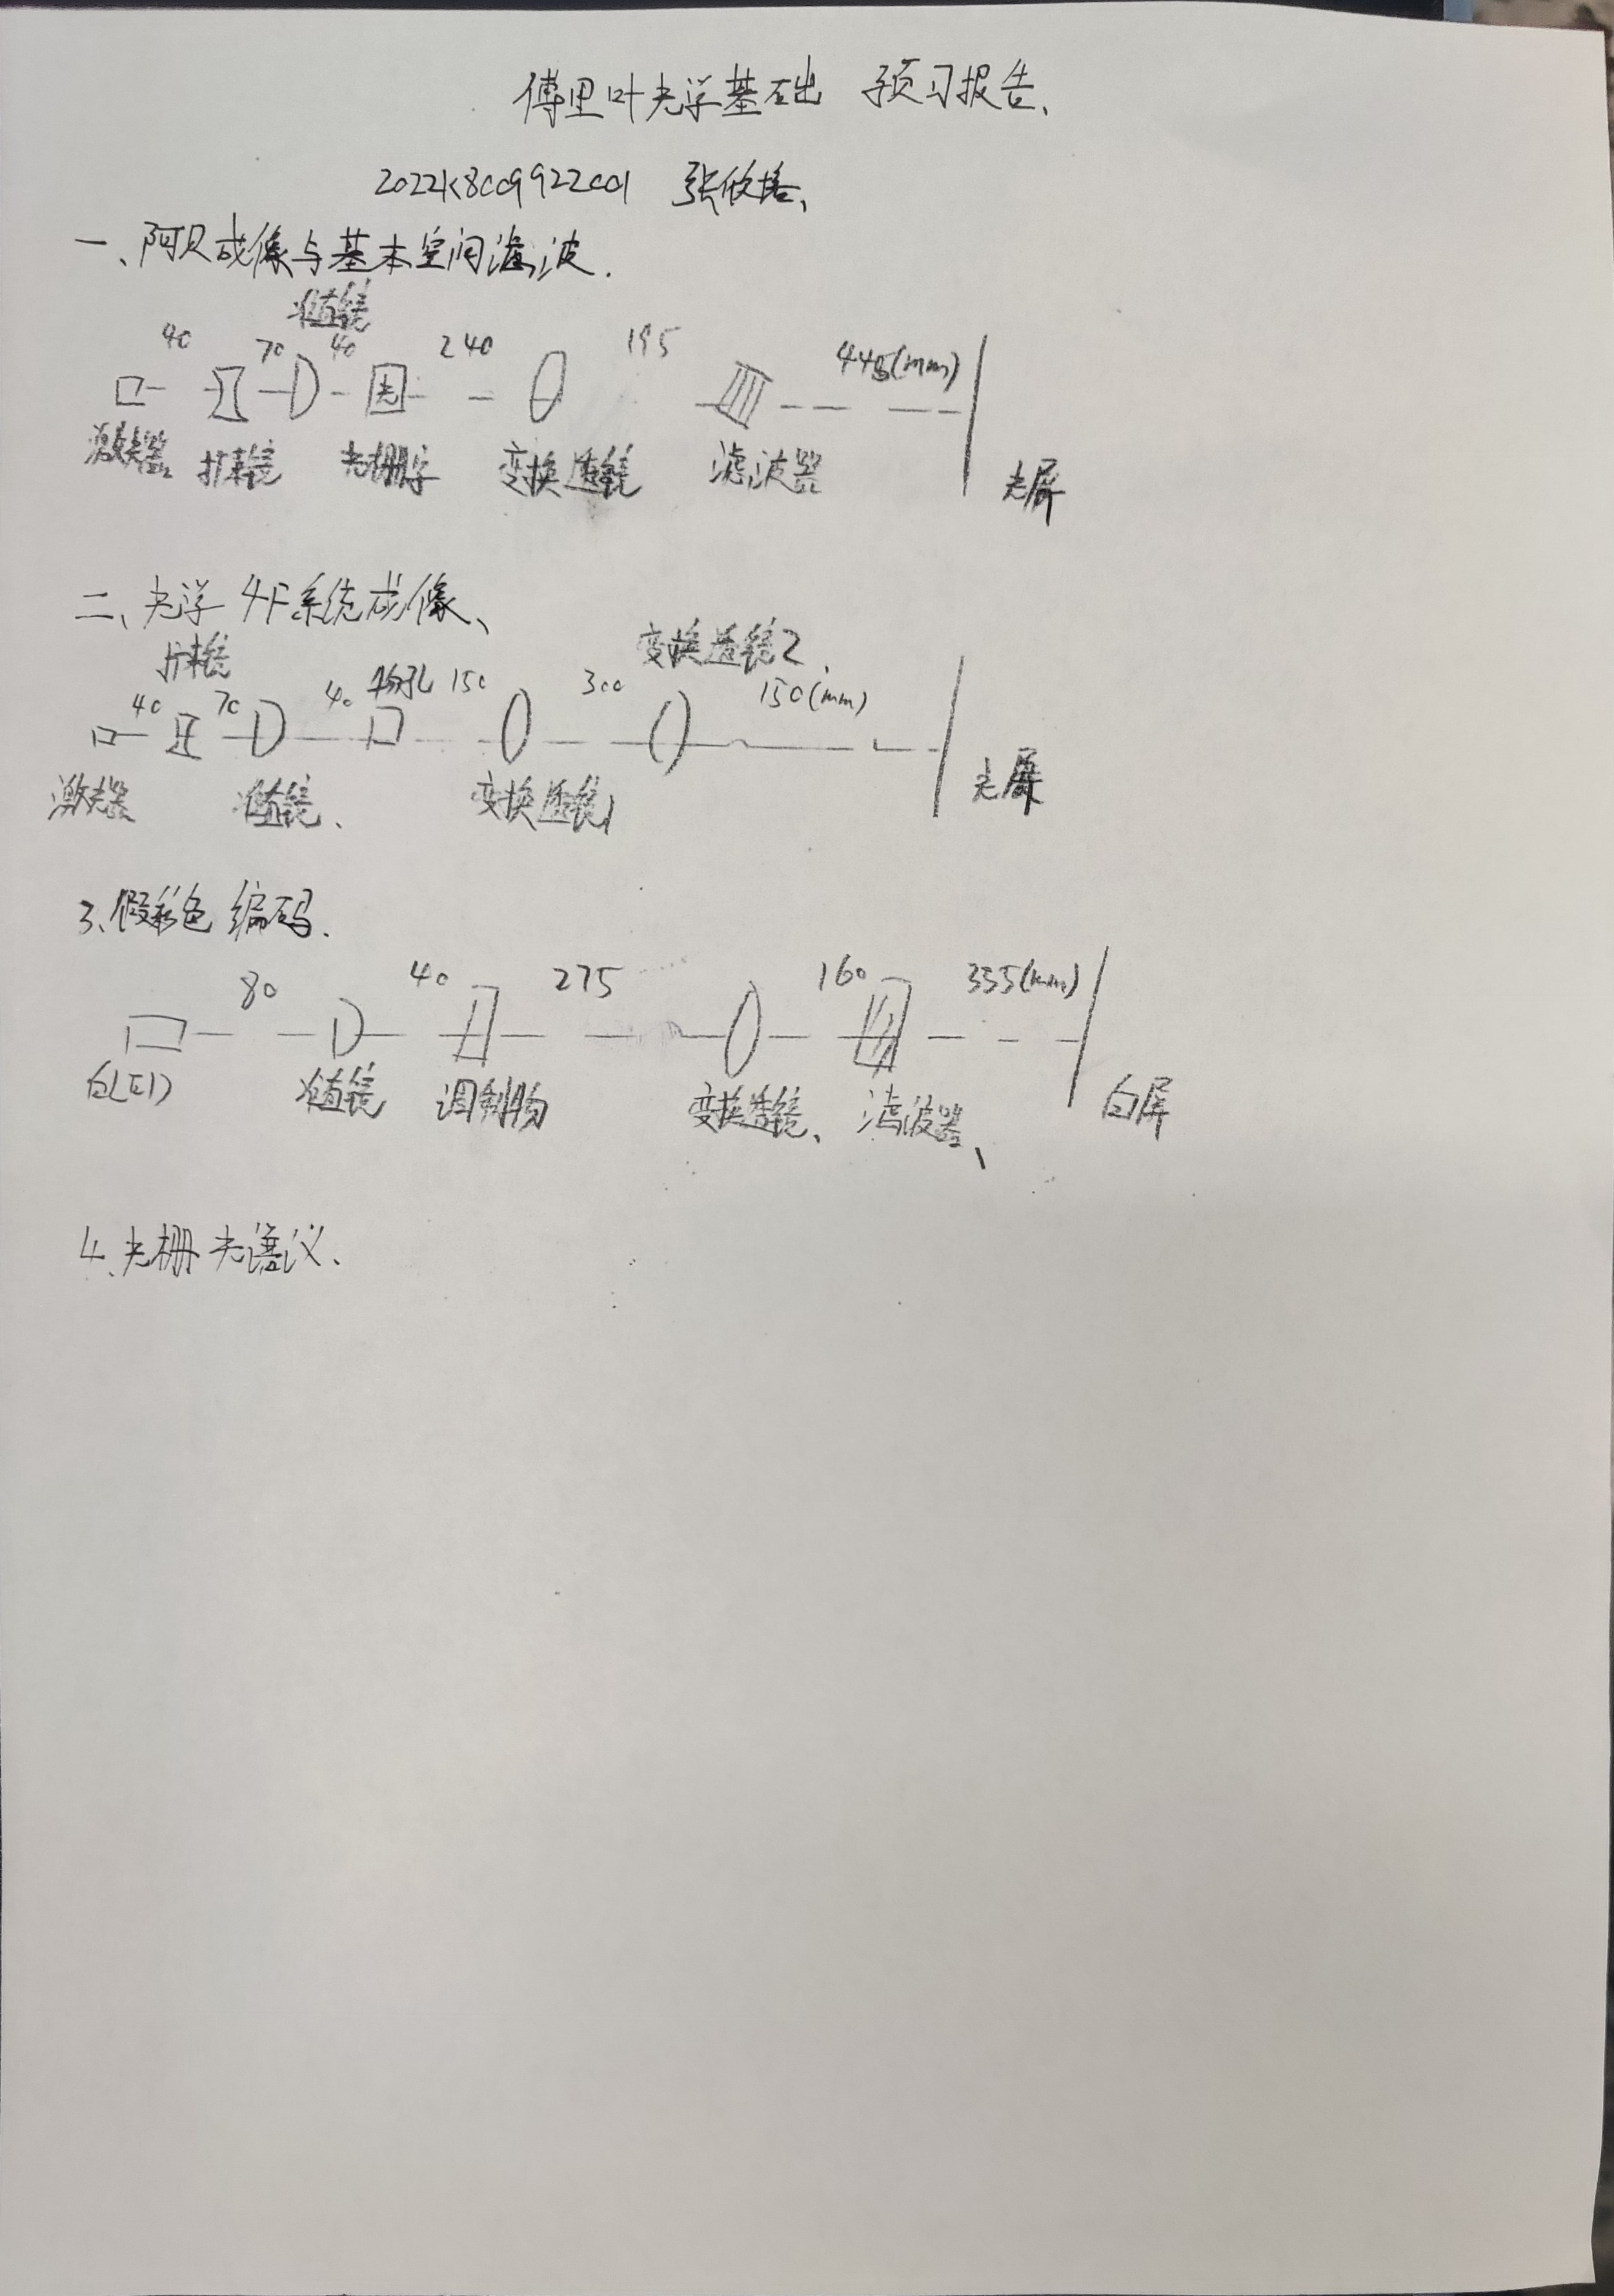
\includegraphics[width=13.5cm]{Fig/0-预习报告.jpg}
\end{figure}

\section{实验目的}

\begin{enumerate}
    \item 掌握一维导轨上光路的调节。
    \item 通过搭建阿贝成像光路和观察不同空间滤波器的效果,体会和理解成像过程、频谱面、谱空间与实空间对应关系、空间滤波、衍射等物理概念。
    \item 体会和掌握光学 4F成像系统的组织和搭建;在前面阿贝成像实验的基础上,进一步体会更为复杂的光学信息处理。
    \item 在基本空间滤波的基础上,进一步体会光栅衍射的色散效果和选频滤波操作,掌握调制假彩色编码的选频滤波和色散选区滤波的原理;并利用提前预制分区信息的光栅图案,实现该图像的假彩色编码。
    \item 根据光栅衍射的原理,测量光栅常数。
    \item 认识手持式光栅光谱仪,使用其测量白光,红光,蓝光,绿光的光谱,使用软件处理数据。
\end{enumerate}

\section{实验器材}

    一维光路导轨,激光器,白光LED,棱镜夹持器,凸透镜(80mm,150mm,175mm),凹透镜(10mm),滤波器,光栅字(10线/mm),天安门光栅(100线/mm),光栅(随机线密度),白屏,滤波器(低通、方向滤波),干板架、滑块、支杆和套筒,手持式光栅光谱仪,电脑,白纸,刻刀,垫板,笔。

\section{实验原理}
\begin{enumerate}
    \item 阿贝成像与基本空间滤波
    \par \hspace*{2em}  阿贝成像原理在原有波动光学衍射和干涉概念的基础上,通过数学上引入傅里叶变换方
    程,通过物理上引入频谱面、频谱花样与物信息的关联关系等概念,为空间滤波和操作提供
    了有力理解工具,并为傅里叶变换光学奠定了基础。阿贝成像原理的主要价值是很好地理解
    和体现了透镜成像的傅里叶变换效果,并把握了频谱面的存在和其重要价值。
    \par \hspace*{2em} 3个点状衍射斑$S_0,S_{+1},S_{-1}$,其偏轴距离满足$S_{\pm1}=\pm F\ tan\theta_i,sin\theta_i=f_i\lambda$;这三个相干点光源成为新的次级光源,然后发射球面波。
    \par \hspace*{2em} 干涉场像最终结果为
    \begin{equation}
        U_{im}\left(x',y'\right)=Ke^{ik\frac{{x'}^2+{y'}^2}{2z}}A_1\left(t_0+t_i\cos2\pi {f'}_ix'\right)
    \end{equation}
    \par \hspace*{2em} 物原本的单频信息 $f_i$可以在像面重构为相似的但是空间频率为 ${f'}_i$的信号,其比值 $V=\frac{{f'}_i}{f_i}$ 就是放大率。
    \begin{figure}[H]
        \centering
        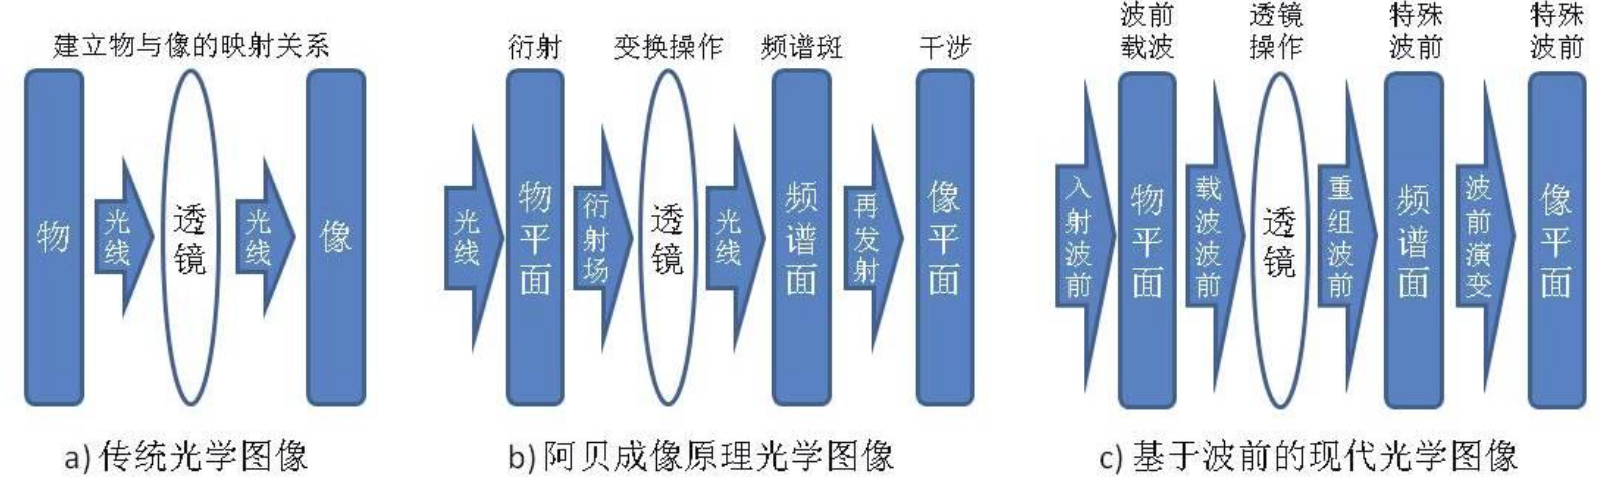
\includegraphics[width=14cm]{Fig/1.png}
        \caption{对于透镜成像的不同理解与图像}
    \end{figure}
    \begin{figure}[H]
        \centering
        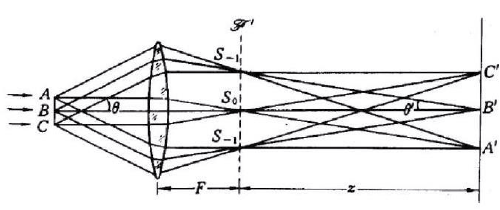
\includegraphics[width=8cm]{Fig/2.png}
        \caption{阿贝成像原理说明图}
    \end{figure}
    \item 光学4F系统成像
    \par \hspace*{2em} “4F”指此系统中的元件距离共有四倍焦距。4F图像处理系统使用两个透镜依次实现傅里叶变换和反傅里叶变换的光学操作,把成像要素与频谱操作要素分离开,是一种可控性、保真性、稳定性更好的相干光学处理系统。
    \par \hspace*{2em} 在 4F图像处理系统下,物场函数处于透镜 1(傅里叶变换透镜)的焦距处,因此其像面位置(在不考虑透镜 2的情况下)在透镜 1后无限远处,即上面公式中的 $z=\infty$,此时上
    面公式中多出的相位函数$e^{ik\frac{{x'}^2+{y'}^2}{2z}}$蜕变成为 1。透镜 2(反傅里叶变换透镜)只是把无限远
    处的无限大的像重新整合到了后焦面处。在无滤波和放大倍率为 1时, 4F图像处理系统所成的像场函数是严格(包括相位)复制了物场函数的。
    \begin{figure}[H]
        \centering
        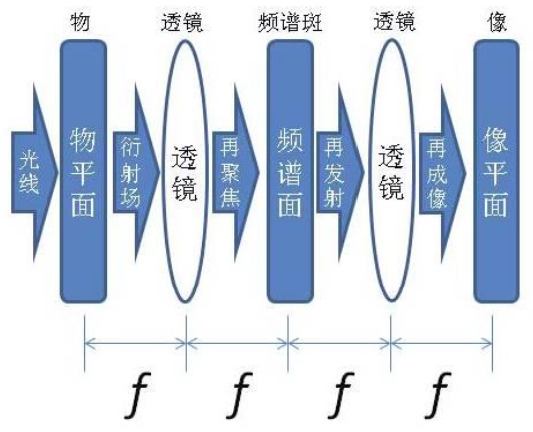
\includegraphics[width=8cm]{Fig/3.png}
        \caption{相干光学处理系统(4F 系统)}
    \end{figure}
    \par \hspace*{2em}一束平行光照射透明物体(待处理的图像),物置于第一个透镜的前焦面处,在第一透镜的后焦面上得到物函数$g(x_0,y_0)$的频谱$G(f_\xi ,f_\eta )$,此
    频谱面又位于第二透镜的前焦面上,在第二透镜的后焦面上得到频谱函数的傅里叶变换
    $g(x, y)$。物函数经过两次傅里叶变换又得到了原函数,只是变成了倒像。在上图中,像平
    面采用的$x, y$坐标与物平面的 $x_0,y_0$坐标的方向相反,因而可以消除由于两次傅里叶变换引
    入的负号。如果在频谱面上插入空间滤波器就可以改变频谱函数,从而使输入信号得到处理。
    \item 假彩色编码
    \par \hspace*{2em}一个白光光源照射透明的天安门 (物面上的被调制物 ),然后携带了物信息的衍射场会继续向前传播,这
    时由于入射光为白光且光栅的衍射行为,不同颜色的光会分散开了,开始呈现多彩颜色;衍
    射场经透镜重新汇聚,在频谱面会形成较清晰的彩色频谱花样;由于天安门花样上不同的区
    域(天空、天安门、草地)的光栅方向是不同的,所以其衍射花样也会延三个不同方向展开,
    呈现出彩色的带状花样。这时,可以选择使用 1)三个不同方向不同颜色(红、绿、蓝)的彩色滤片来过滤不同
    方向的衍射斑条纹; 2)或者也可以使用一张白纸,在其上根据不同部位的衍射斑来选取指
    定的颜色通过;以上两种方法都可以实现不同区域的彩色编码。 由于这种编码方法是利用不
    同方位的光栅对图像不同空间部位进行调制来实现的,故称为$\theta$调制空间假彩色编码。而该
    实验的目标配色结果为绿草地、红天安门和蓝天。
    \item 光栅衍射测量光栅常数实验
    \par \hspace*{2em}光栅衍射中,$d\sin\theta=k\lambda,k=0,\pm1,\pm2...$,$d=\frac{\lambda}{\sin \theta}=\lambda\frac{\sqrt{L^2+{\Delta x}^2}}{\Delta x}$。根据所得的光栅条纹,调整合适的光屏距离,测得$\Delta x$。然后读取光栅和光屏距离L,计算光栅常数d。
    \item 光栅光谱仪测光谱实验
    \par \hspace*{2em}光栅光谱仪是利用光栅得到光谱(即不同光强)的仪器。将入射的复色光经过光栅出射为单色光。
    \par \hspace*{2em}光栅光谱仪的性能参数:角色散率$D=\frac{d\theta}{d\lambda}=\frac{k}{d\sin\theta}$,色分辨率$R=\frac{\lambda}{\Delta \lambda}=kN$,最大衍射角不超过$90^\circ$,$K_{min}=1$,由光栅方程可知$\lambda_{max}<d$,第m级衍射能分辨的最小波长差$\Delta \lambda=\frac{\lambda}{m}$。
\end{enumerate}


\section{实验内容}
\subsection{阿贝成像与基本空间滤波}
\noindent 实验过程:
\begin{enumerate}
    \item 如图和预习报告图搭建光路。调整变换透镜和凹、凸透镜位置,达成准直。
    \begin{figure}[H]
        \centering
        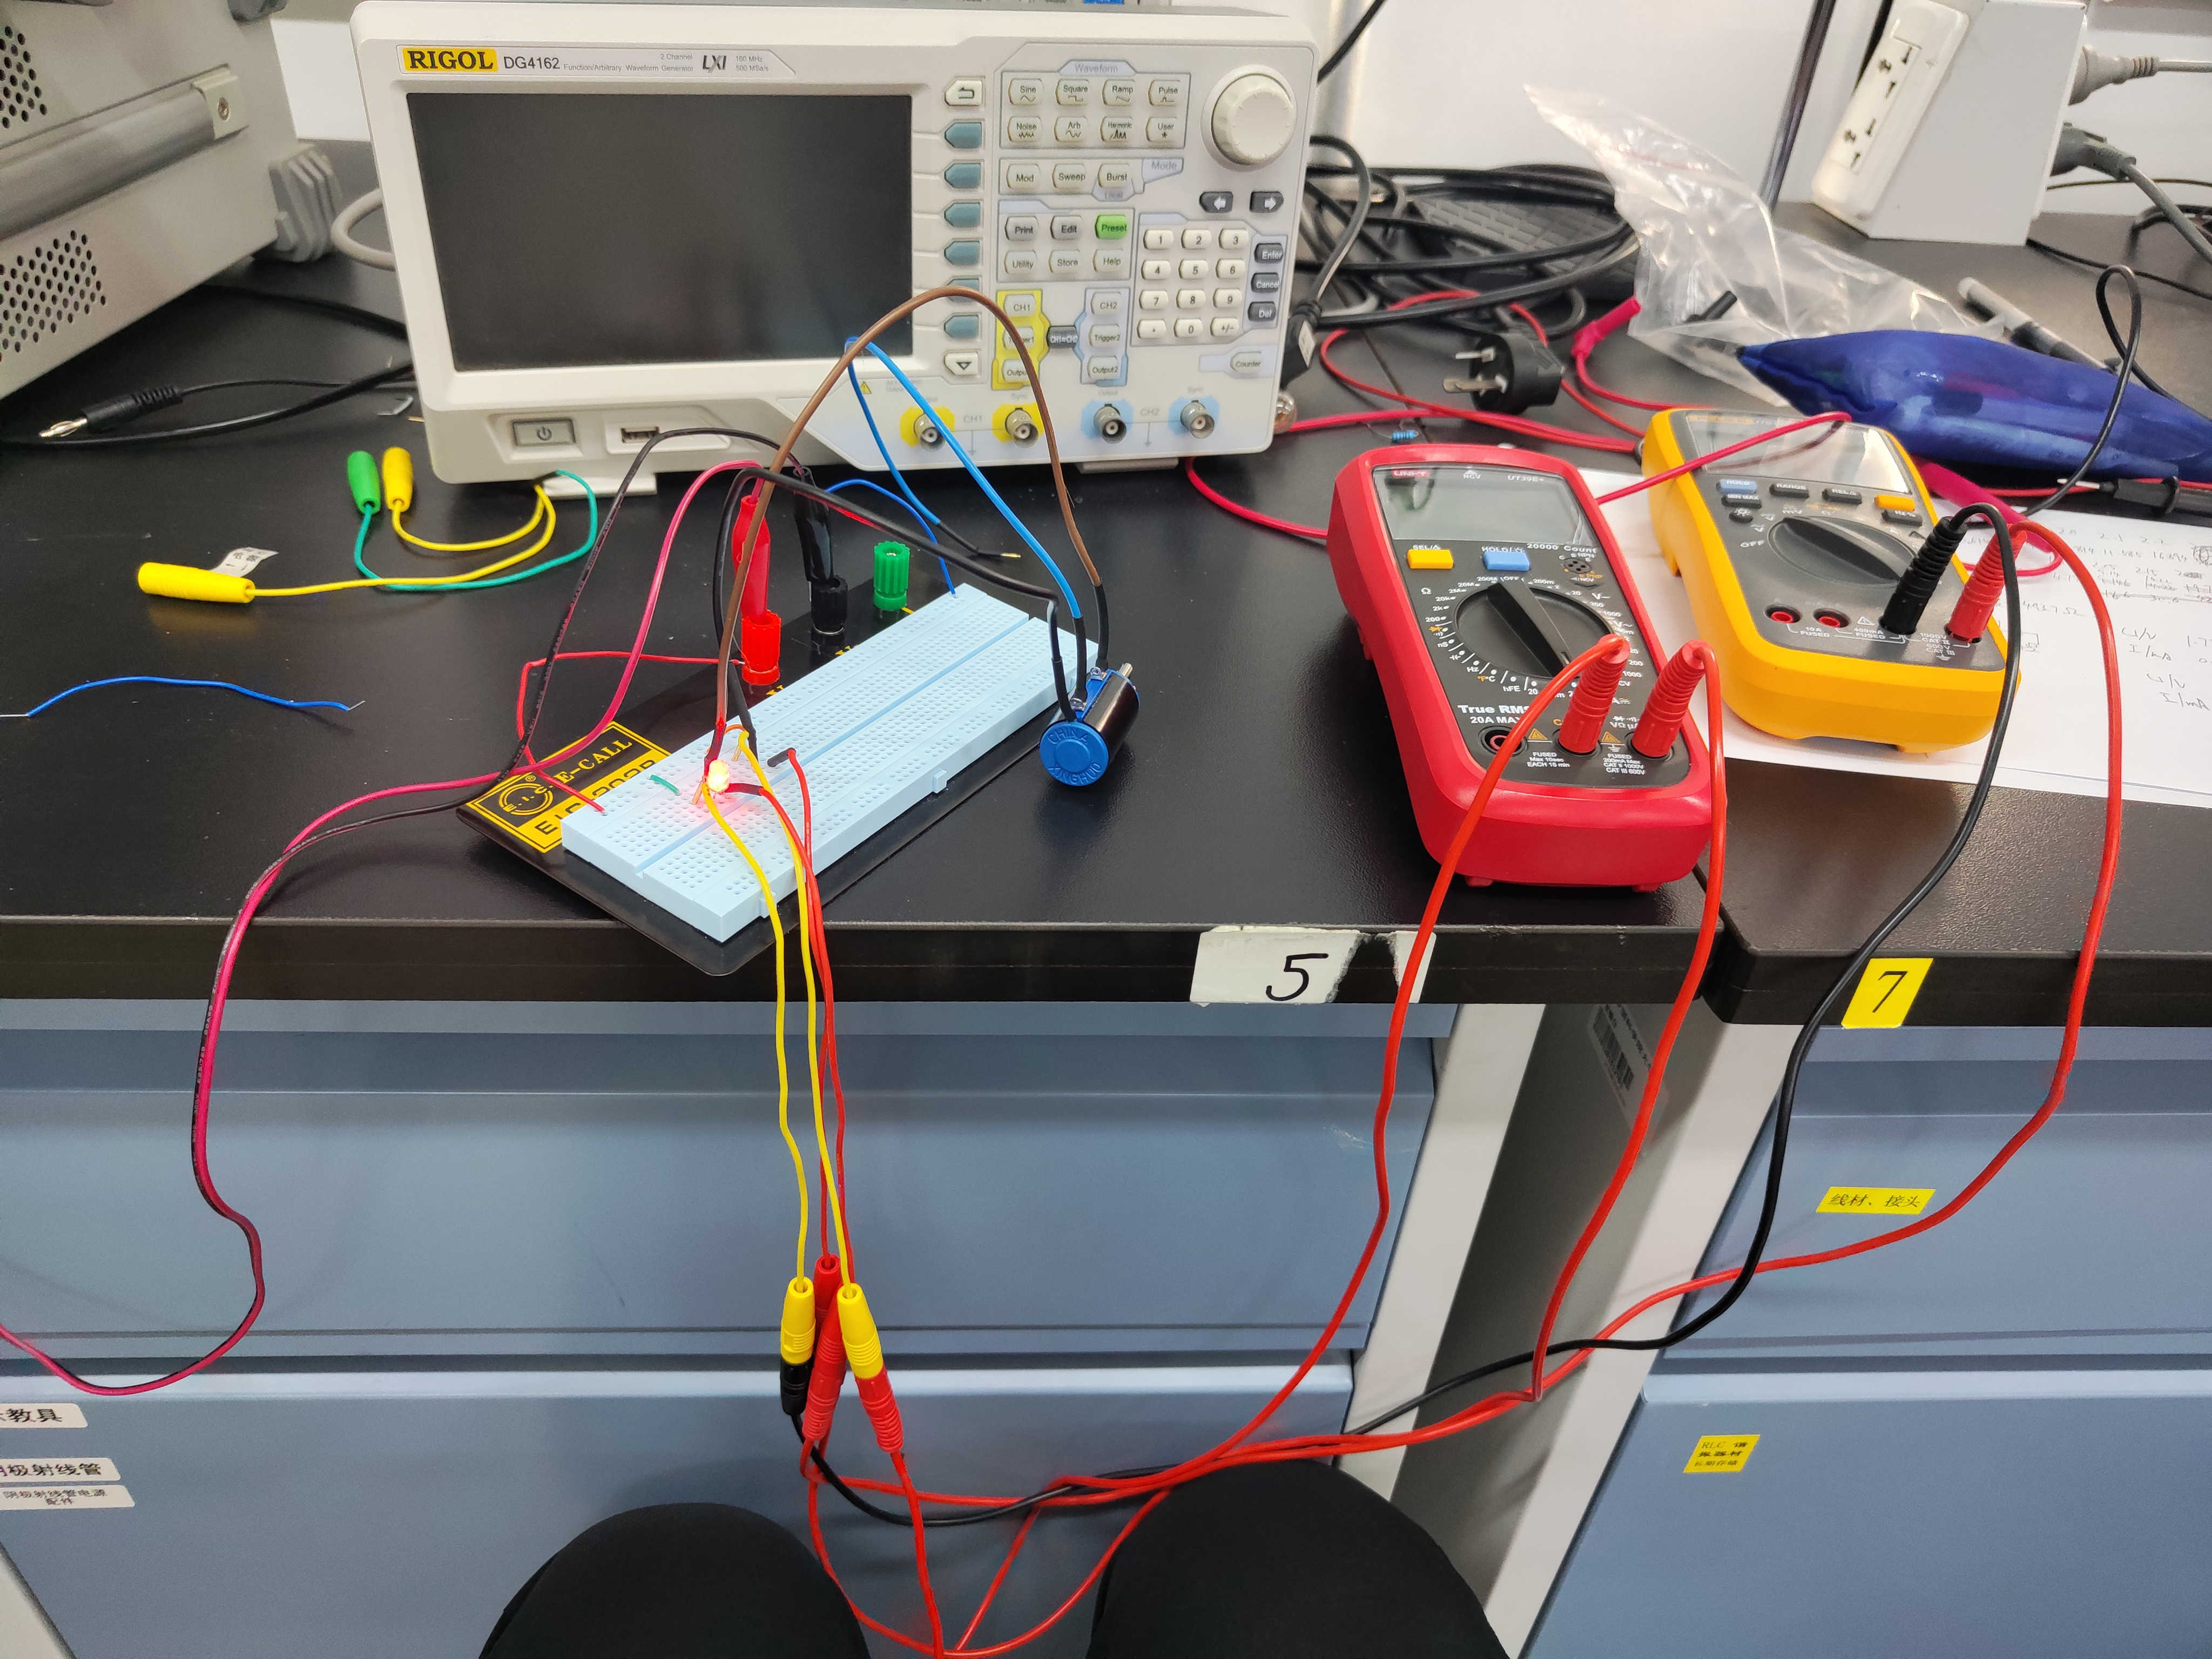
\includegraphics[width=8cm]{Fig/4.jpg}
        \caption{阿贝成像实验光路(省略光屏)}
    \end{figure} 
    \item 读取此时光屏上的像。
    \item 安装滤波器(单孔,长条),调整滤波器角度,读取此时光屏上的像。
    \begin{figure}[H]
        \centering
        \begin{minipage}[t]{0.49\linewidth}
            \centering
            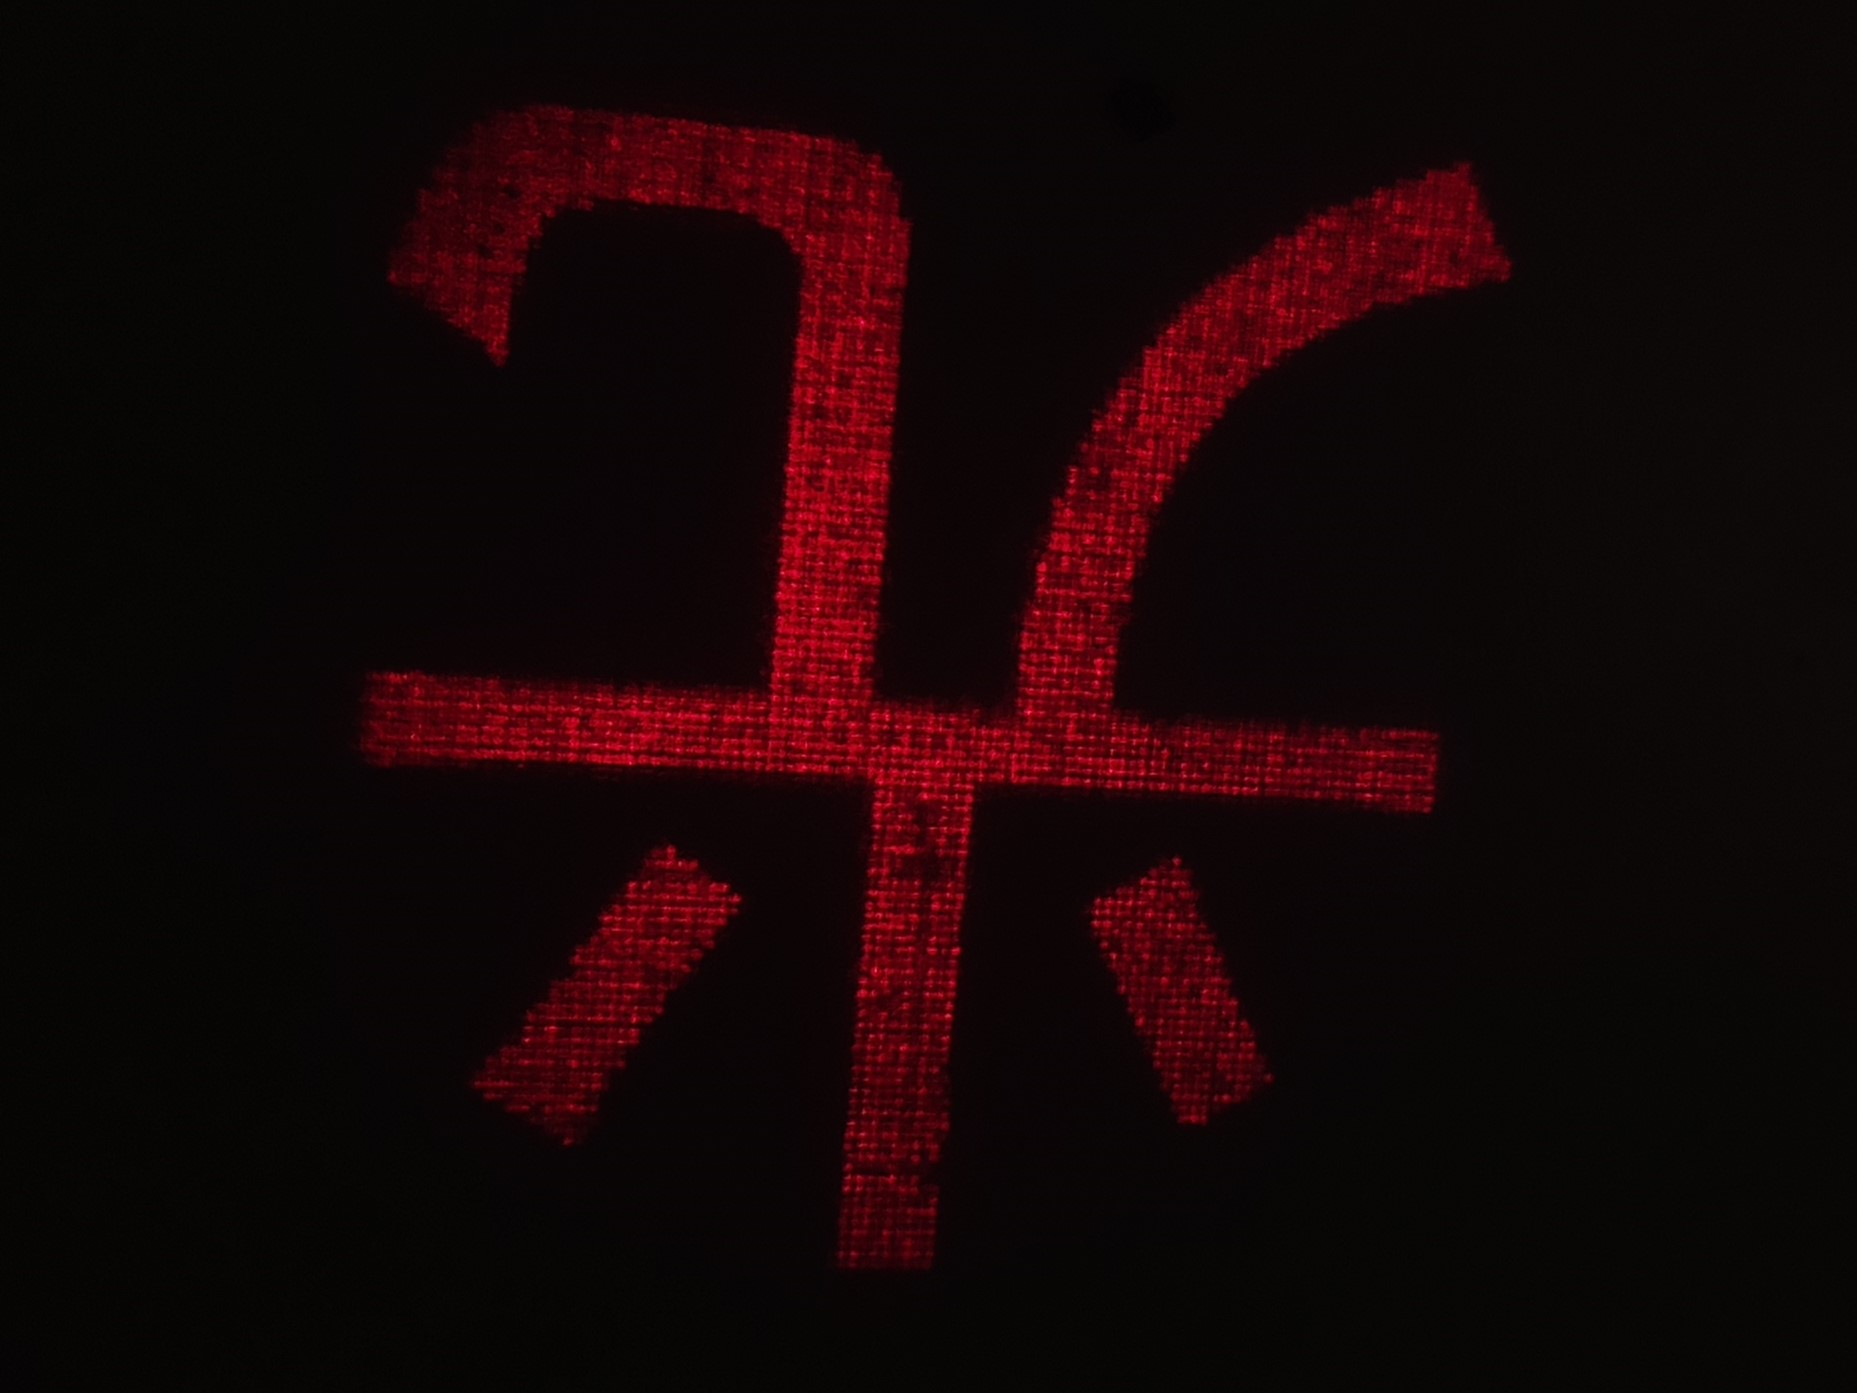
\includegraphics[width=7.5cm]{Fig/5-无滤波器.jpg}
            \caption{无滤波器}
        \end{minipage}
        \begin{minipage}[t]{0.49\linewidth}
            \centering
            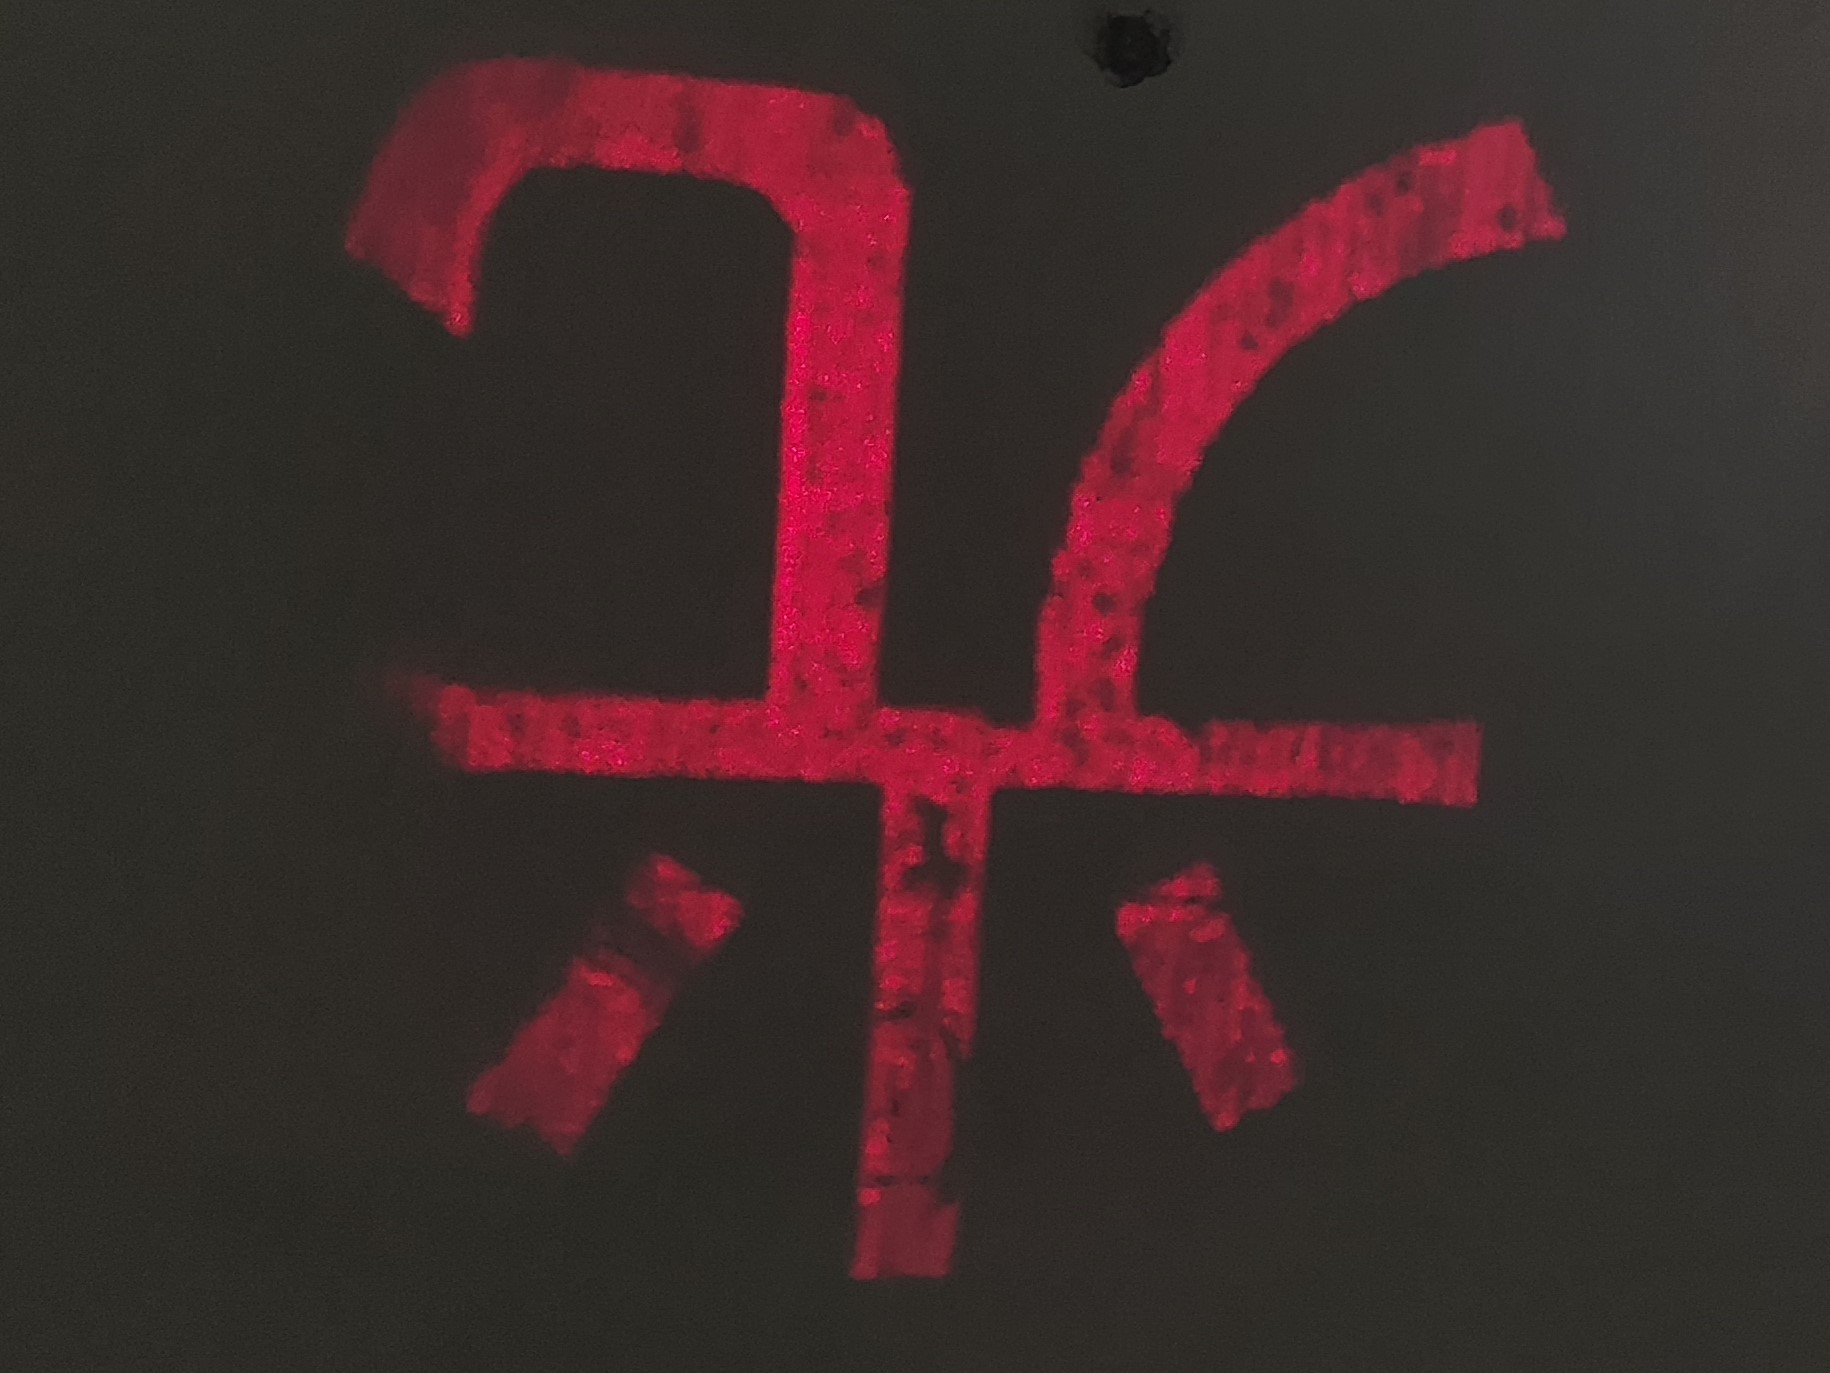
\includegraphics[width=7.5cm]{Fig/5-孔}
            \caption{孔}
        \end{minipage} 
        
    \end{figure}
    \begin{figure}[H]
        \centering
        \begin{minipage}[t]{0.49\linewidth}
            \centering
            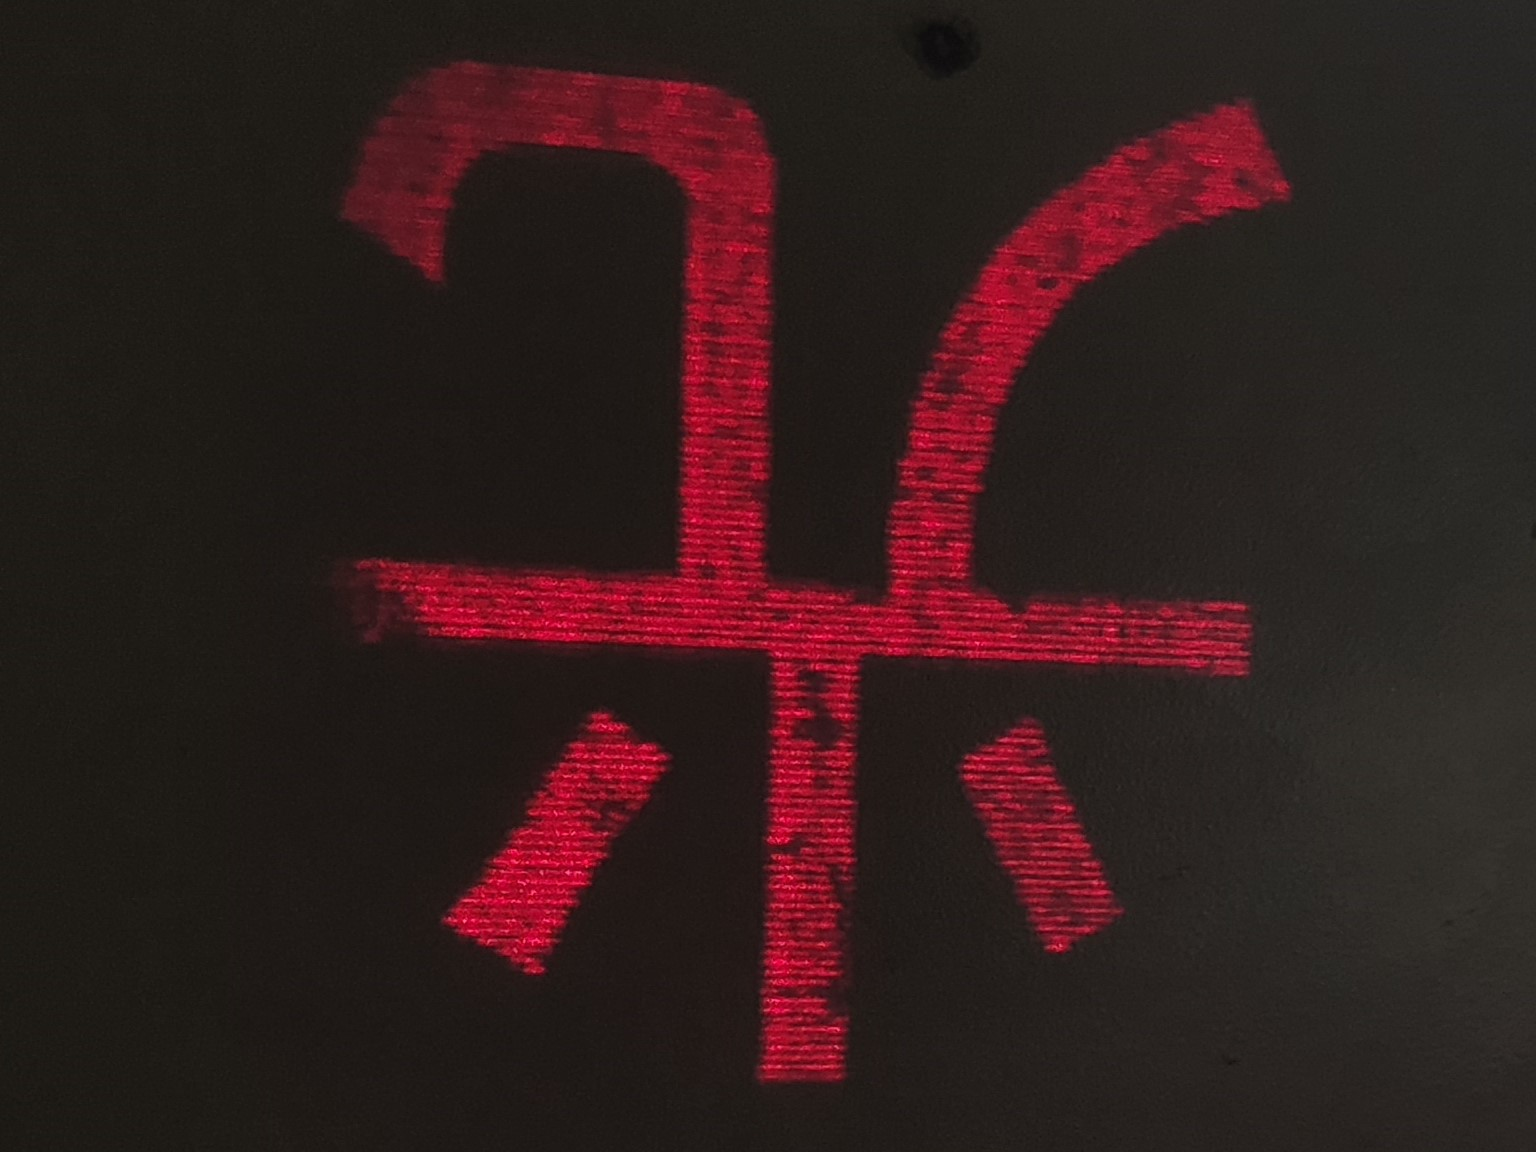
\includegraphics[width=7.5cm]{Fig/5-竖缝.jpg}
            \caption{竖缝}
        \end{minipage}
        \begin{minipage}[t]{0.49\linewidth}
            \centering
            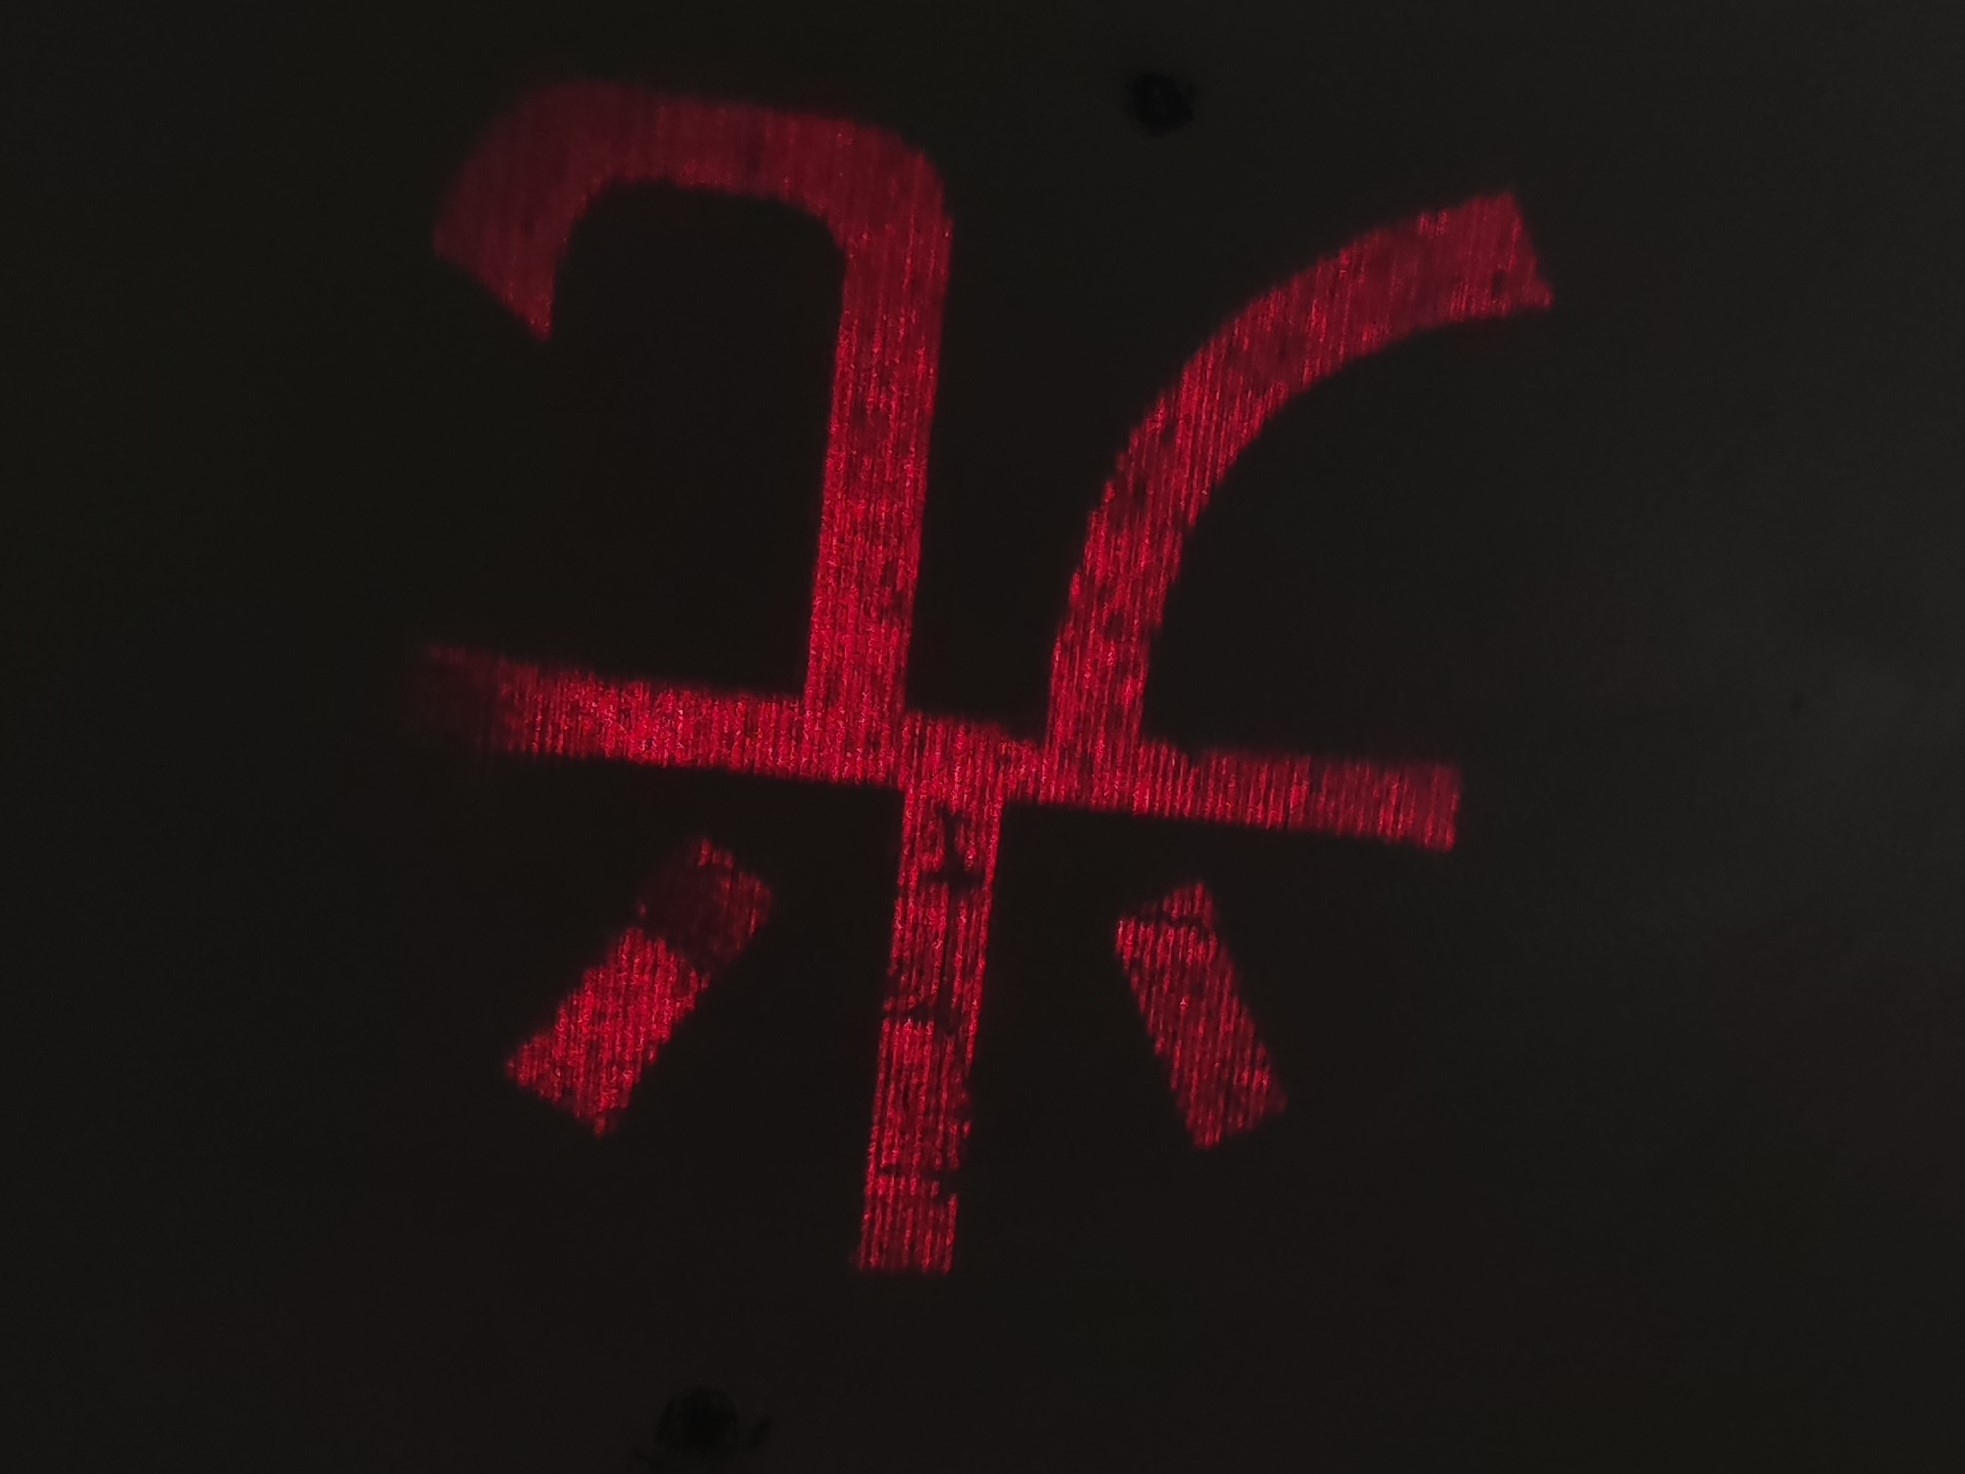
\includegraphics[width=7.5cm]{Fig/5-横缝.jpg}
            \caption{横缝}
        \end{minipage}
    \end{figure}
    \begin{figure}[H]
        \centering
        \begin{minipage}[t]{0.49\linewidth}
            \centering
            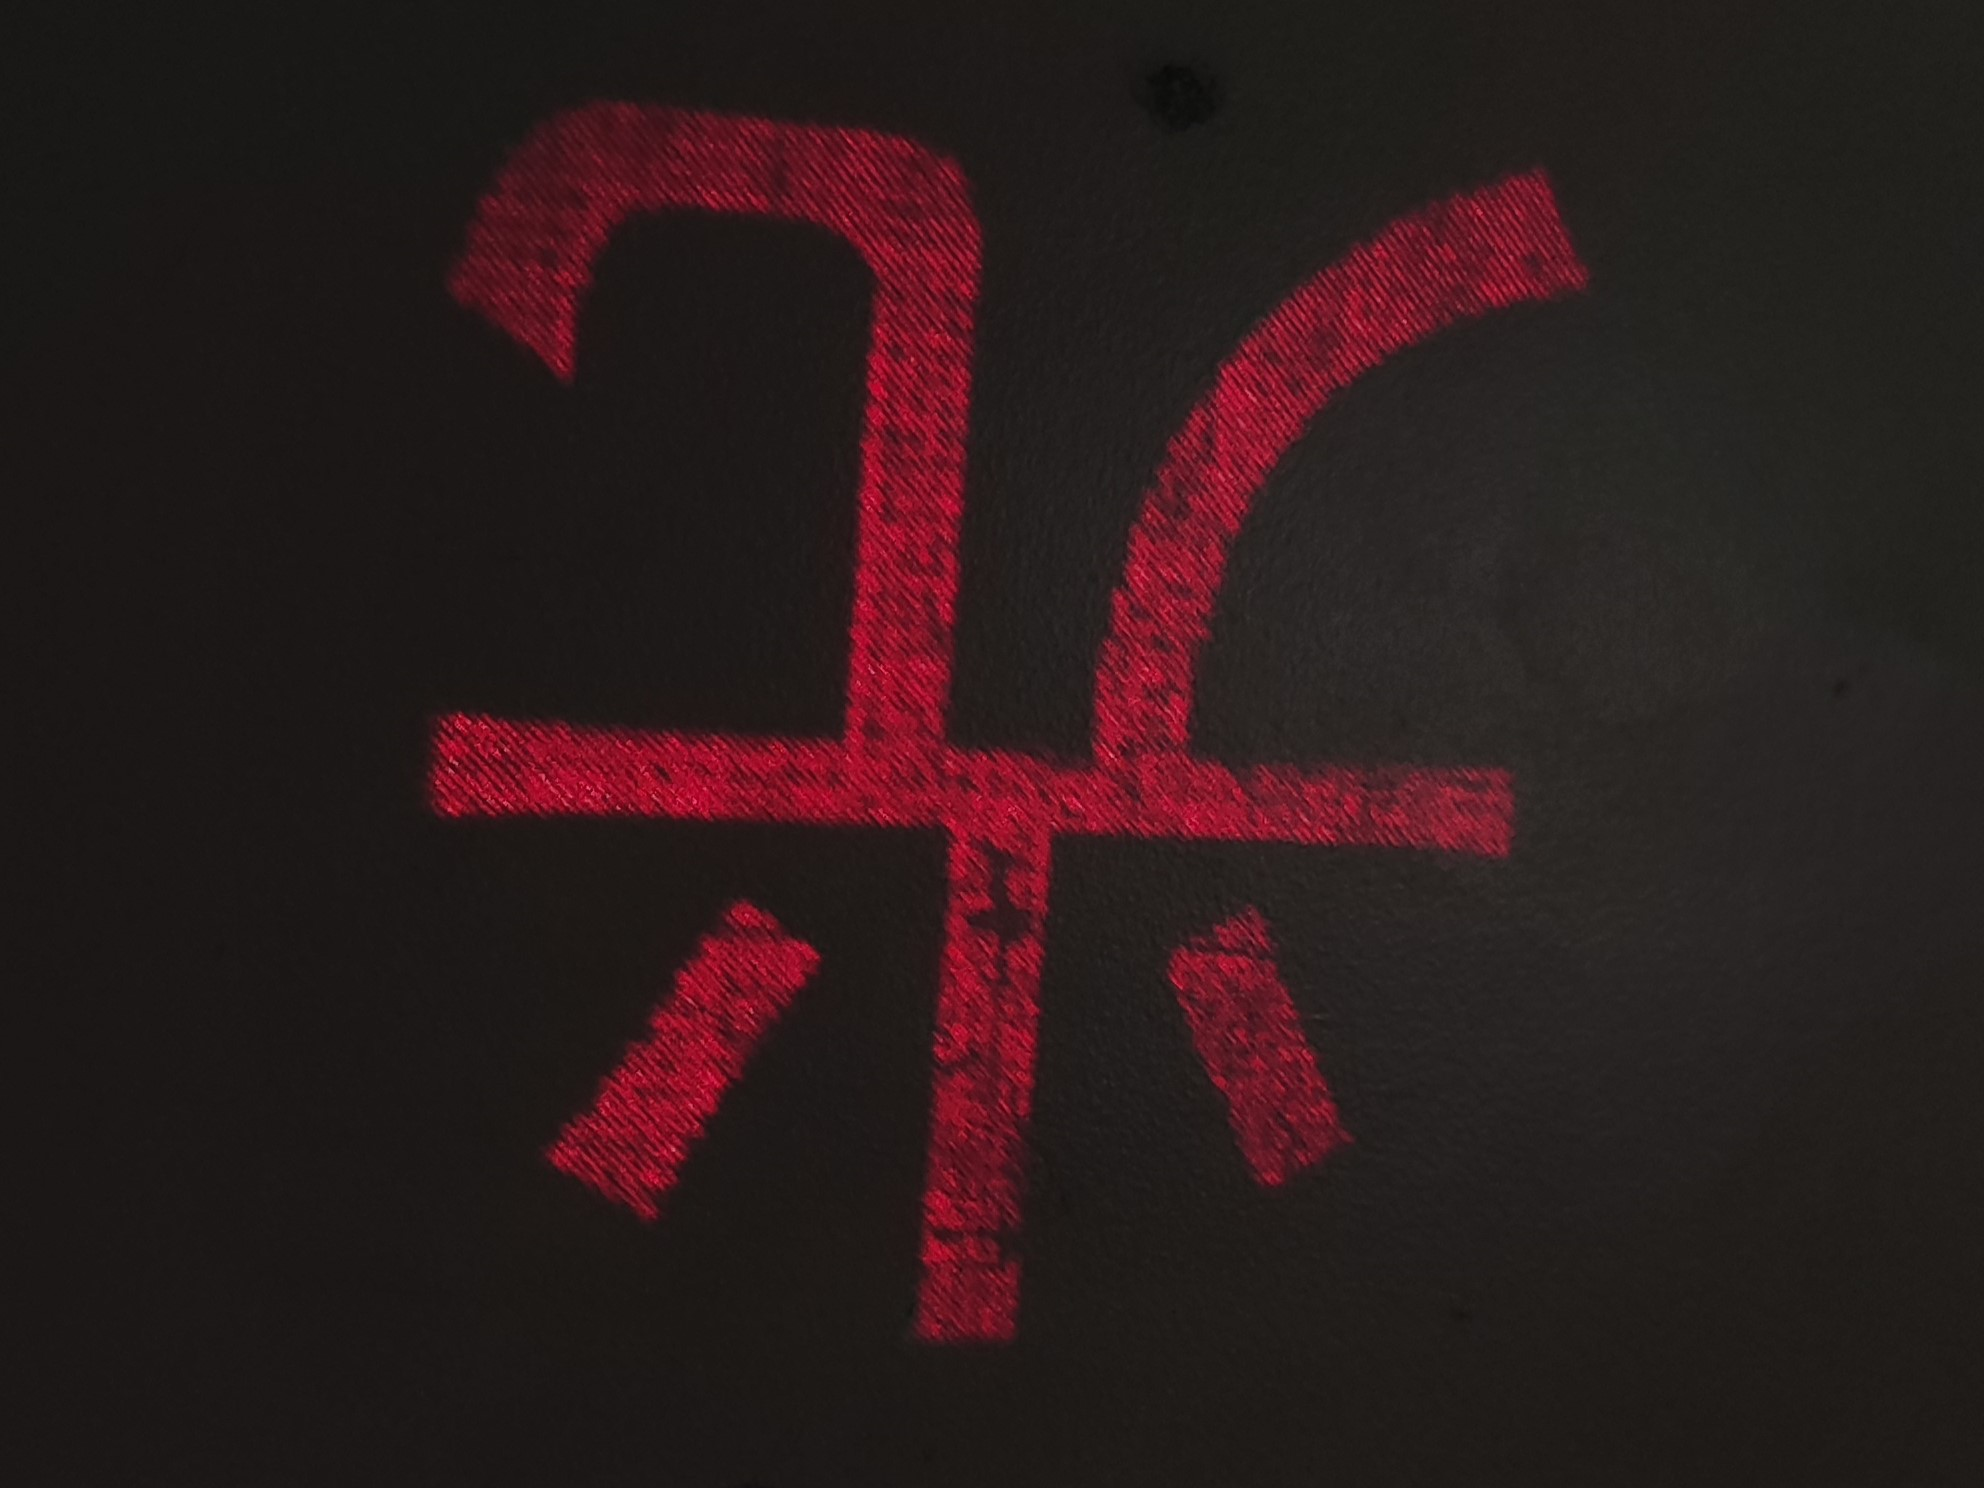
\includegraphics[width=7.5cm]{Fig/5-左斜.jpg}
            \caption{左斜}
        \end{minipage}
        \begin{minipage}[t]{0.49\linewidth}
            \centering
            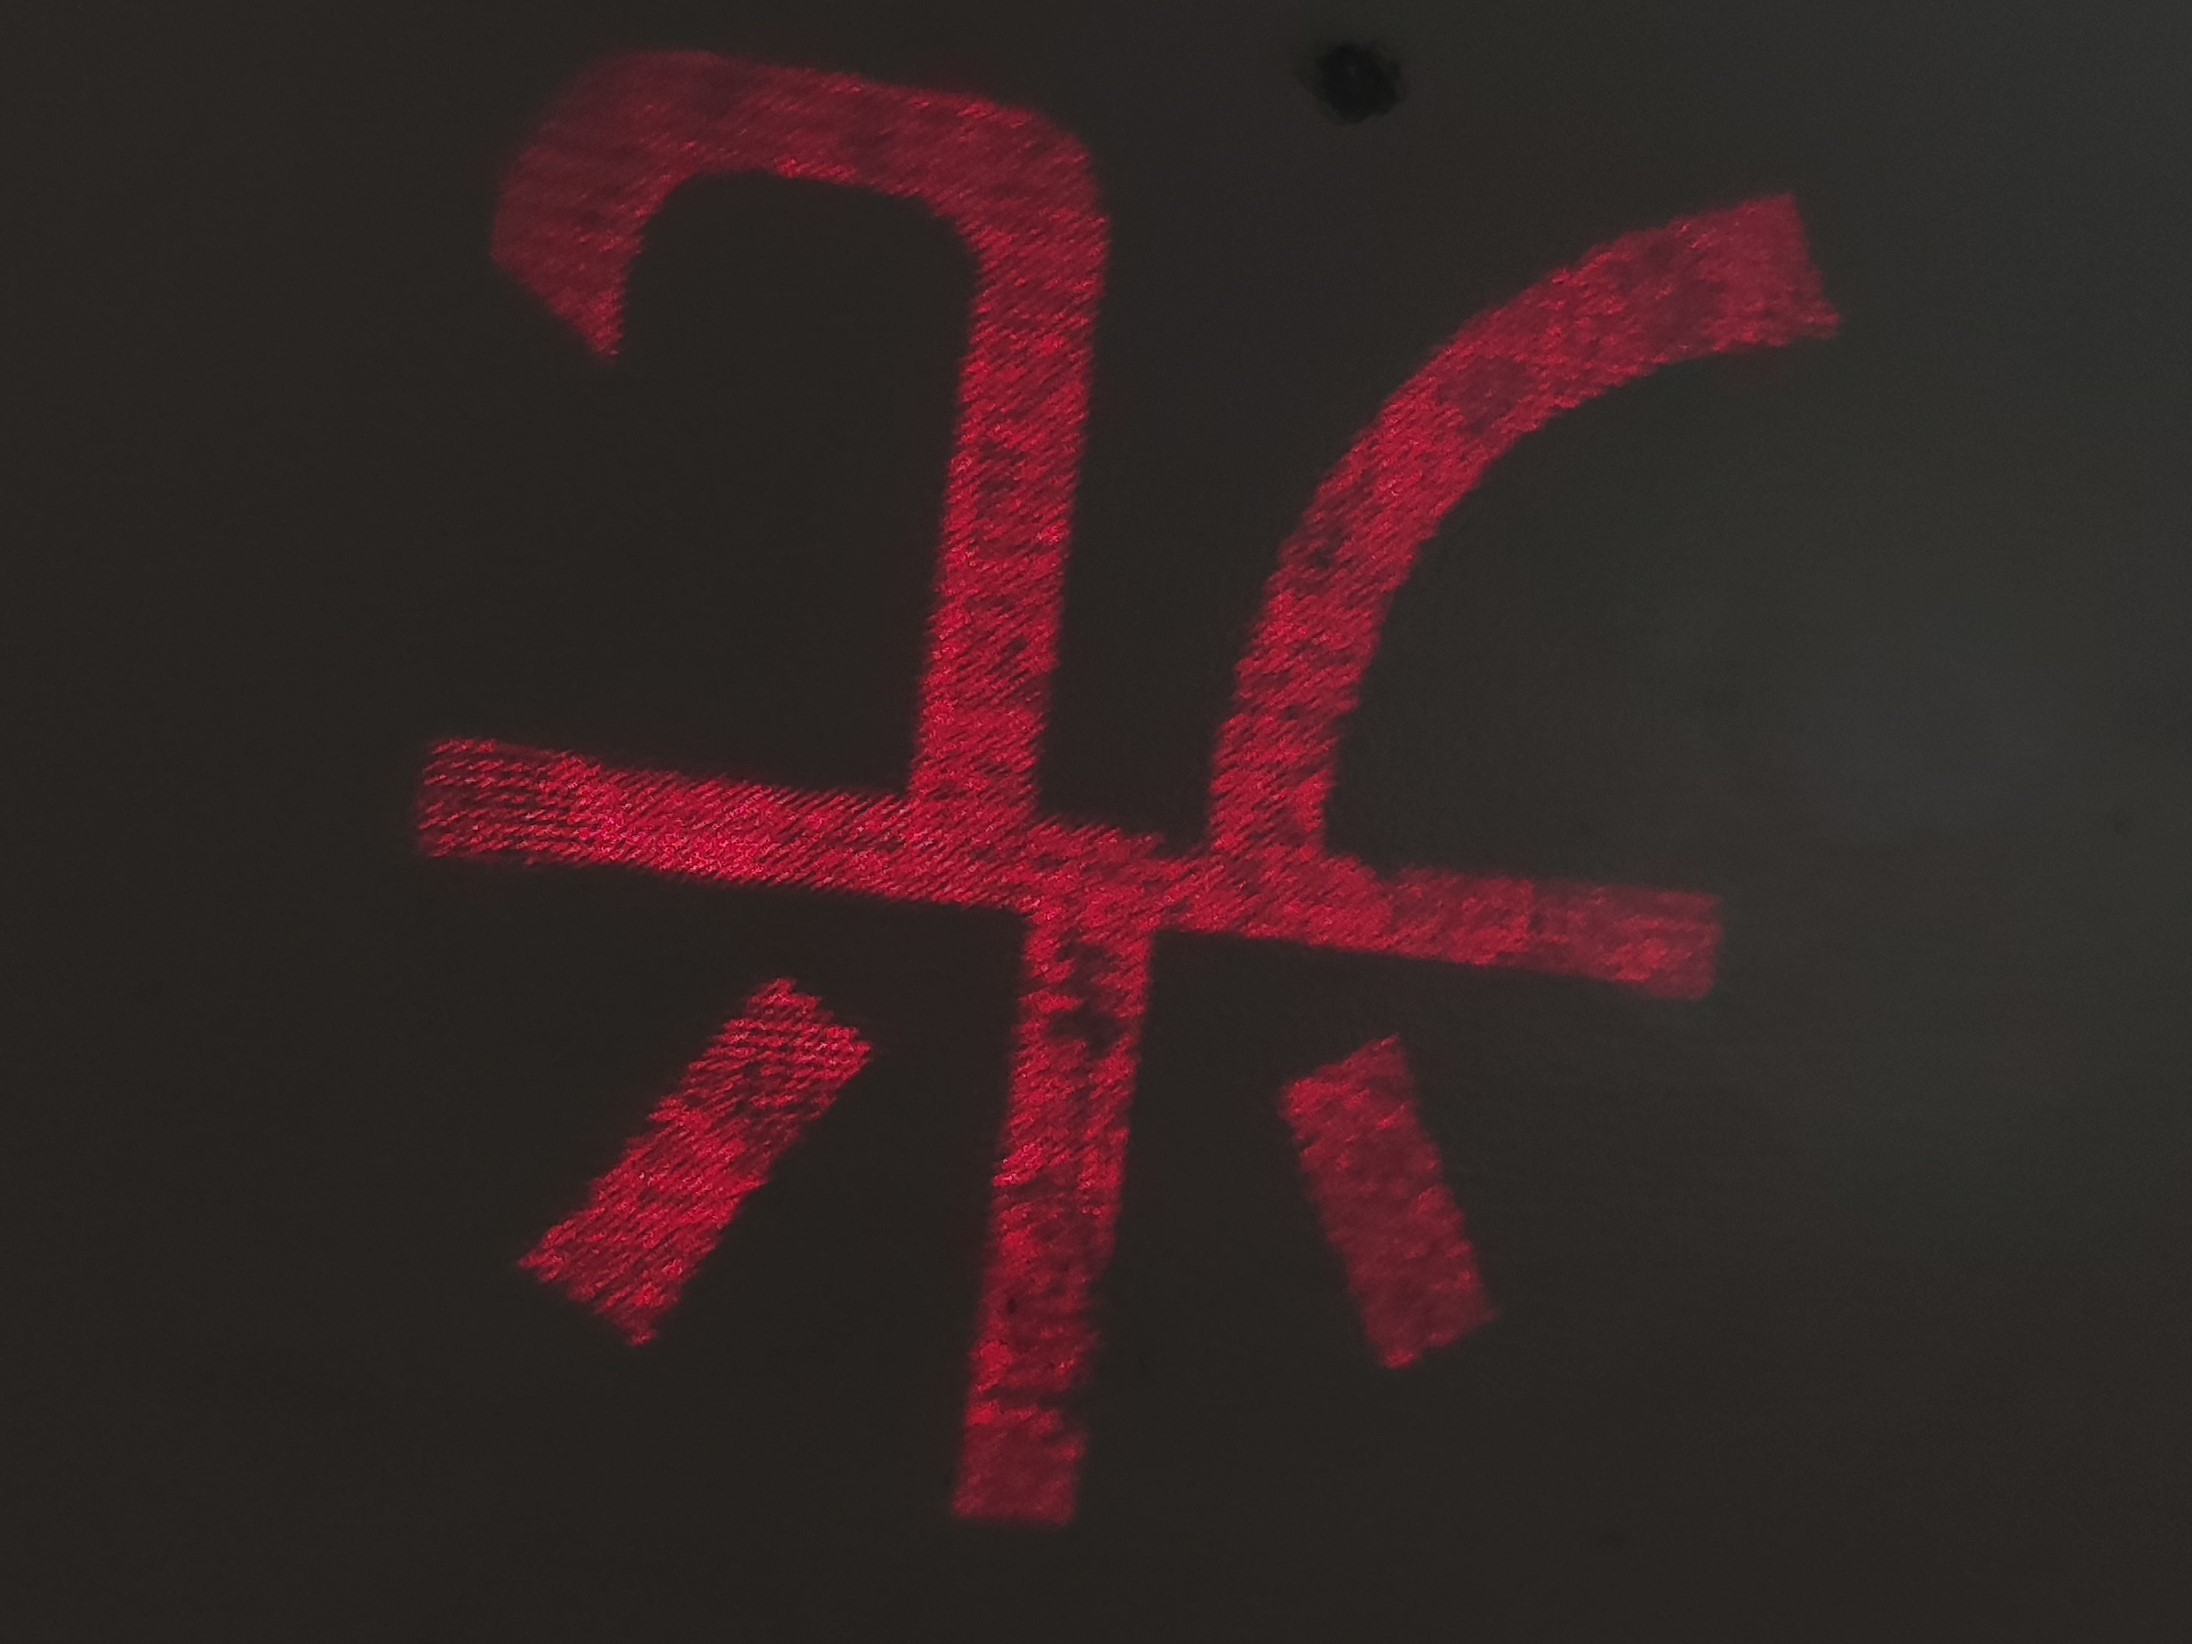
\includegraphics[width=7.5cm]{Fig/5-右斜.jpg}
            \caption{右斜}
        \end{minipage}
    \end{figure}
    \par \hspace*{2em}可以看到,条纹在缝的垂直方向上变宽,而小孔滤波器会使图像全向变宽,即变模糊。这符合我们对衍射规律的认识。
    \begin{figure}[H]
        \centering
        \begin{minipage}[t]{0.3\linewidth}
            \centering
            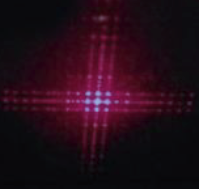
\includegraphics[width=4.4cm]{Fig/6.png}
            \caption{频谱点}
        \end{minipage}
        \begin{minipage}[t]{0.34\linewidth}
            \centering
            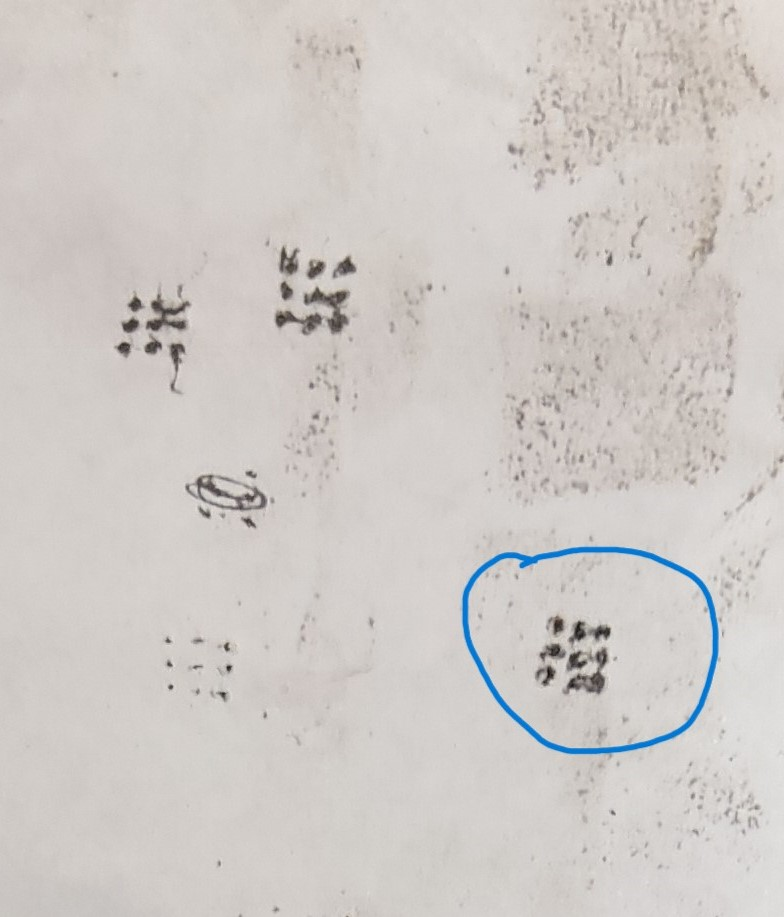
\includegraphics[width=4.4cm]{Fig/7.jpg}
            \caption{高通滤纸(实际使用蓝圈所示)}
        \end{minipage}
        \begin{minipage}[t]{0.35\linewidth}
            \centering
            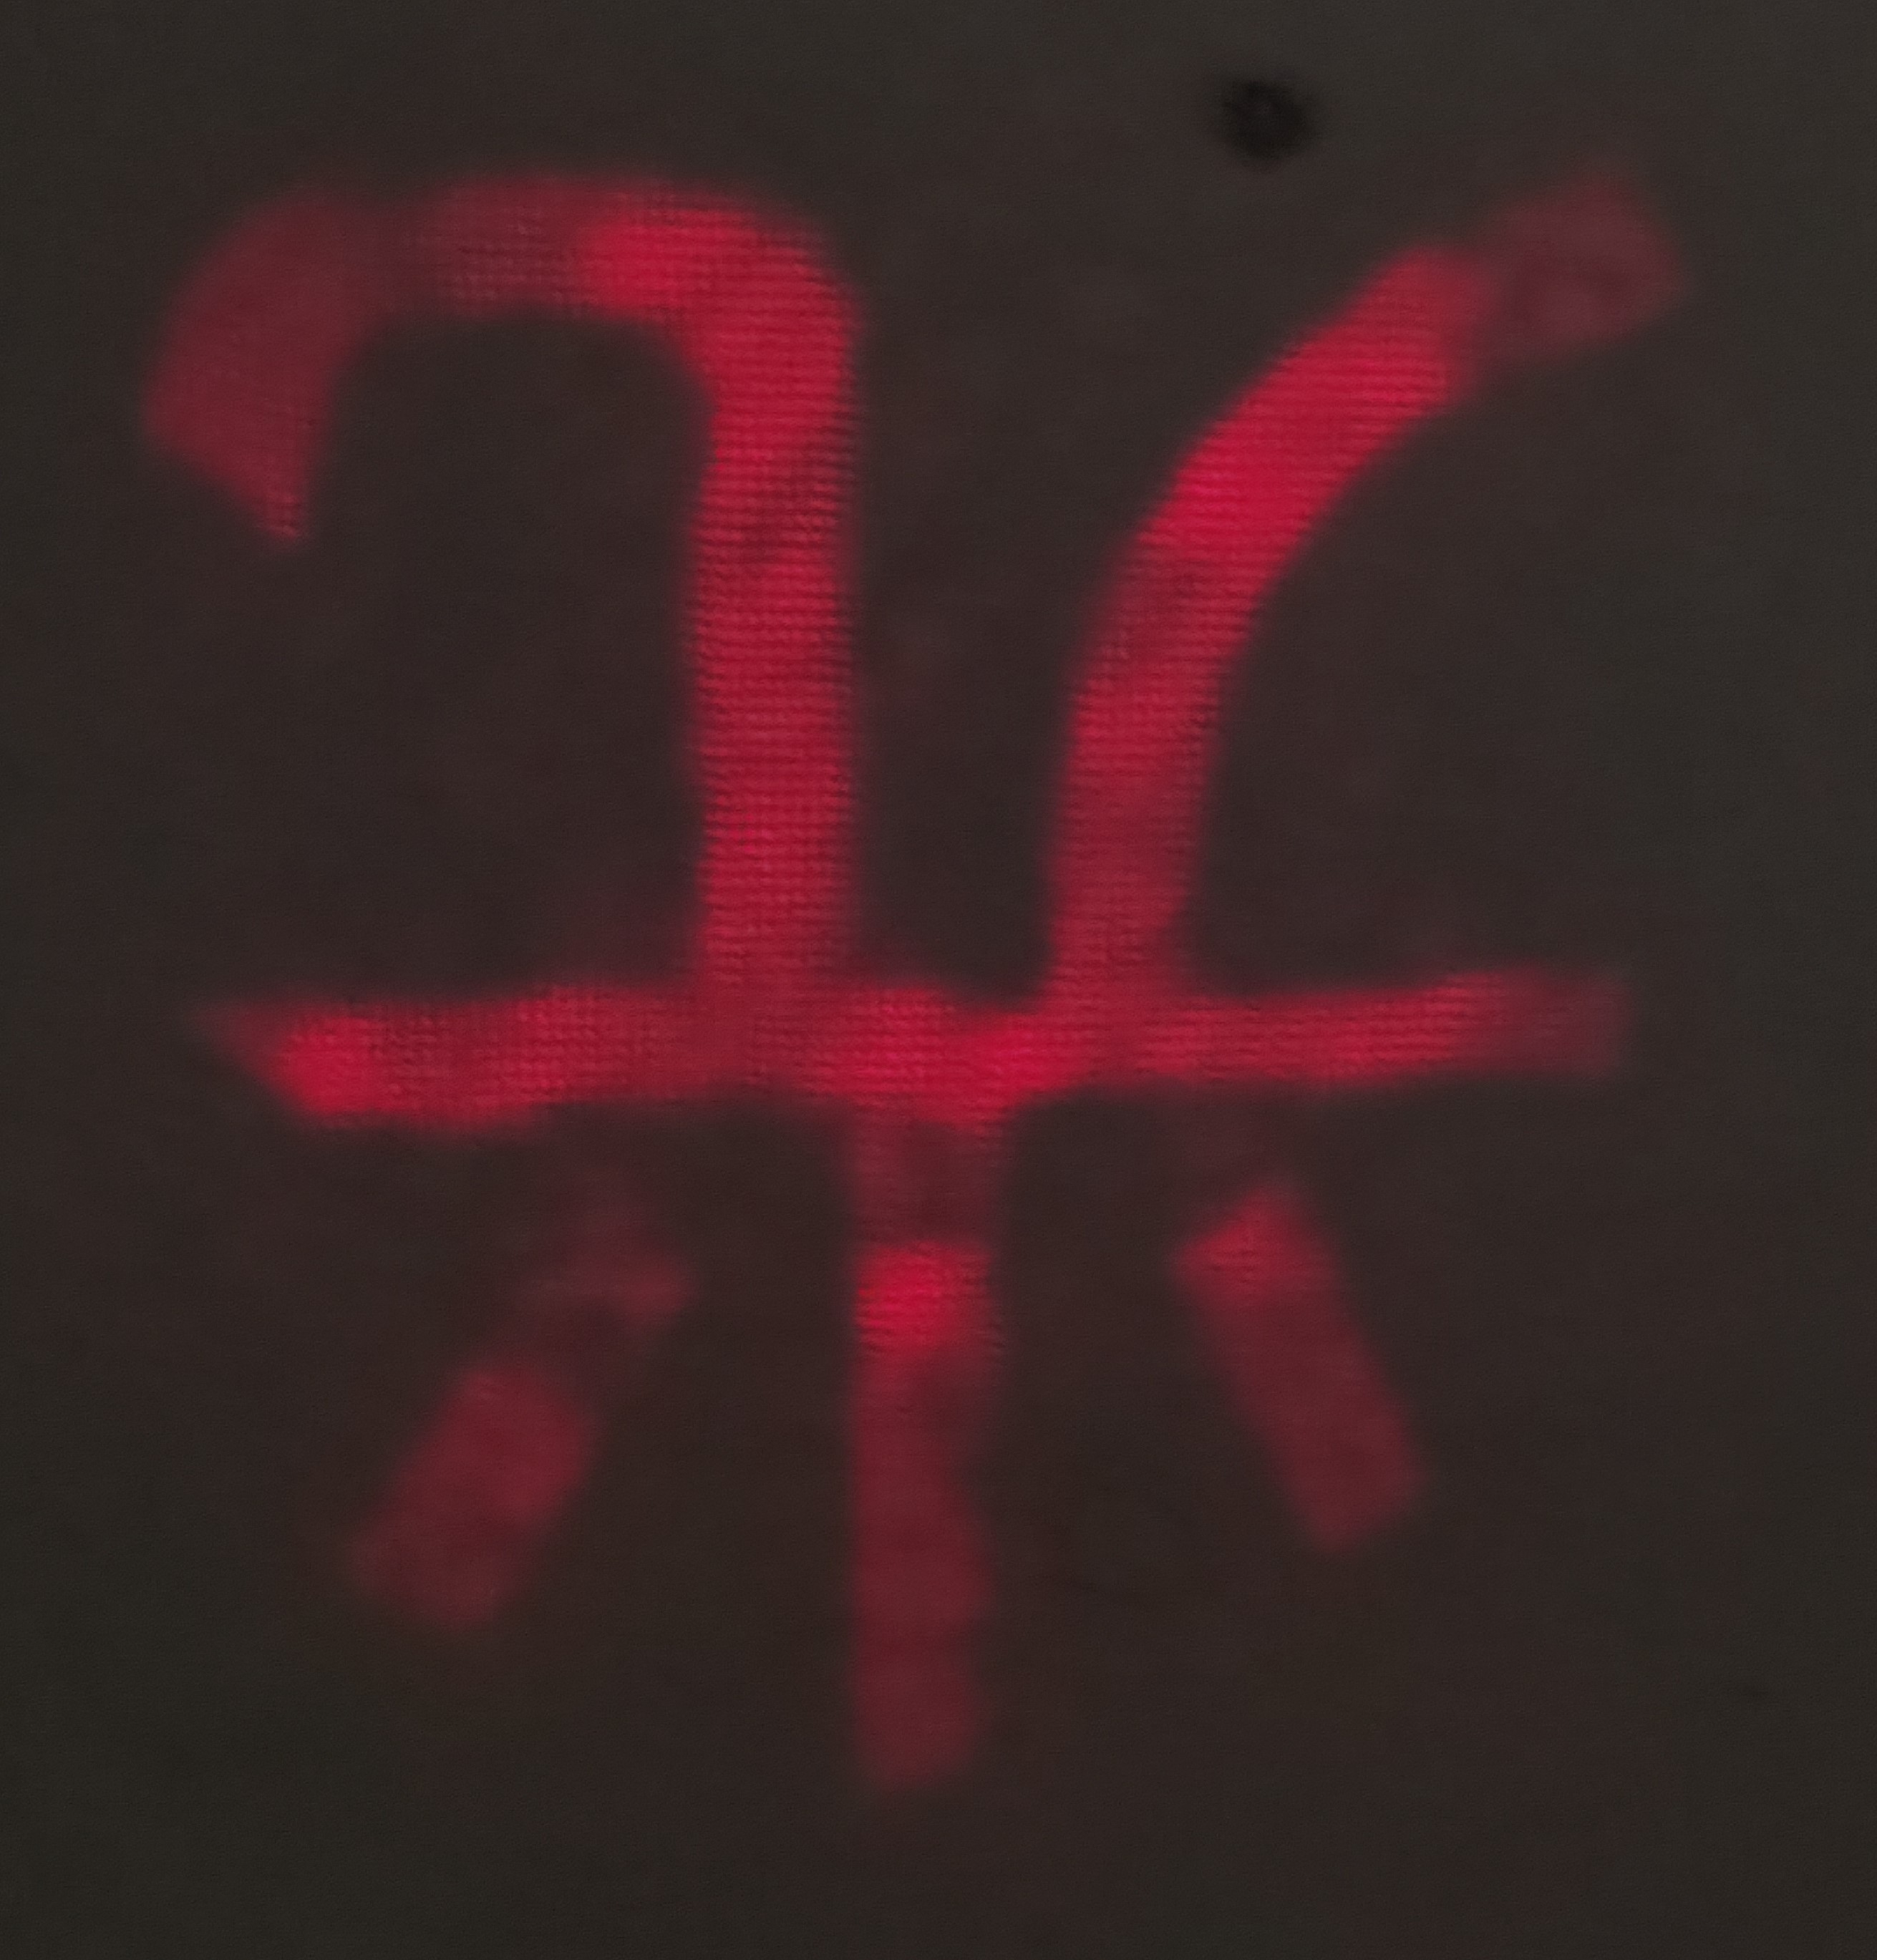
\includegraphics[height=5cm]{Fig/8-高通.jpg}
            \caption{高通}
        \end{minipage}
    \end{figure}
    \par \hspace*{2em} 由频谱点中间九个点,在纸上刻画出高通滤纸,仅滤过中心九个点,如图。所得衍射图像部分保持圆形点阵结构。但由于手刻的洞精度不足,所得图像不是很清晰。
\end{enumerate}



\subsection{光学4F系统成像}
\noindent 实验过程:
\begin{enumerate}
    \item 如图和预习报告图搭建光路。调整凹、凸透镜位置,达成准直。
    \begin{figure}[H]
        \centering
        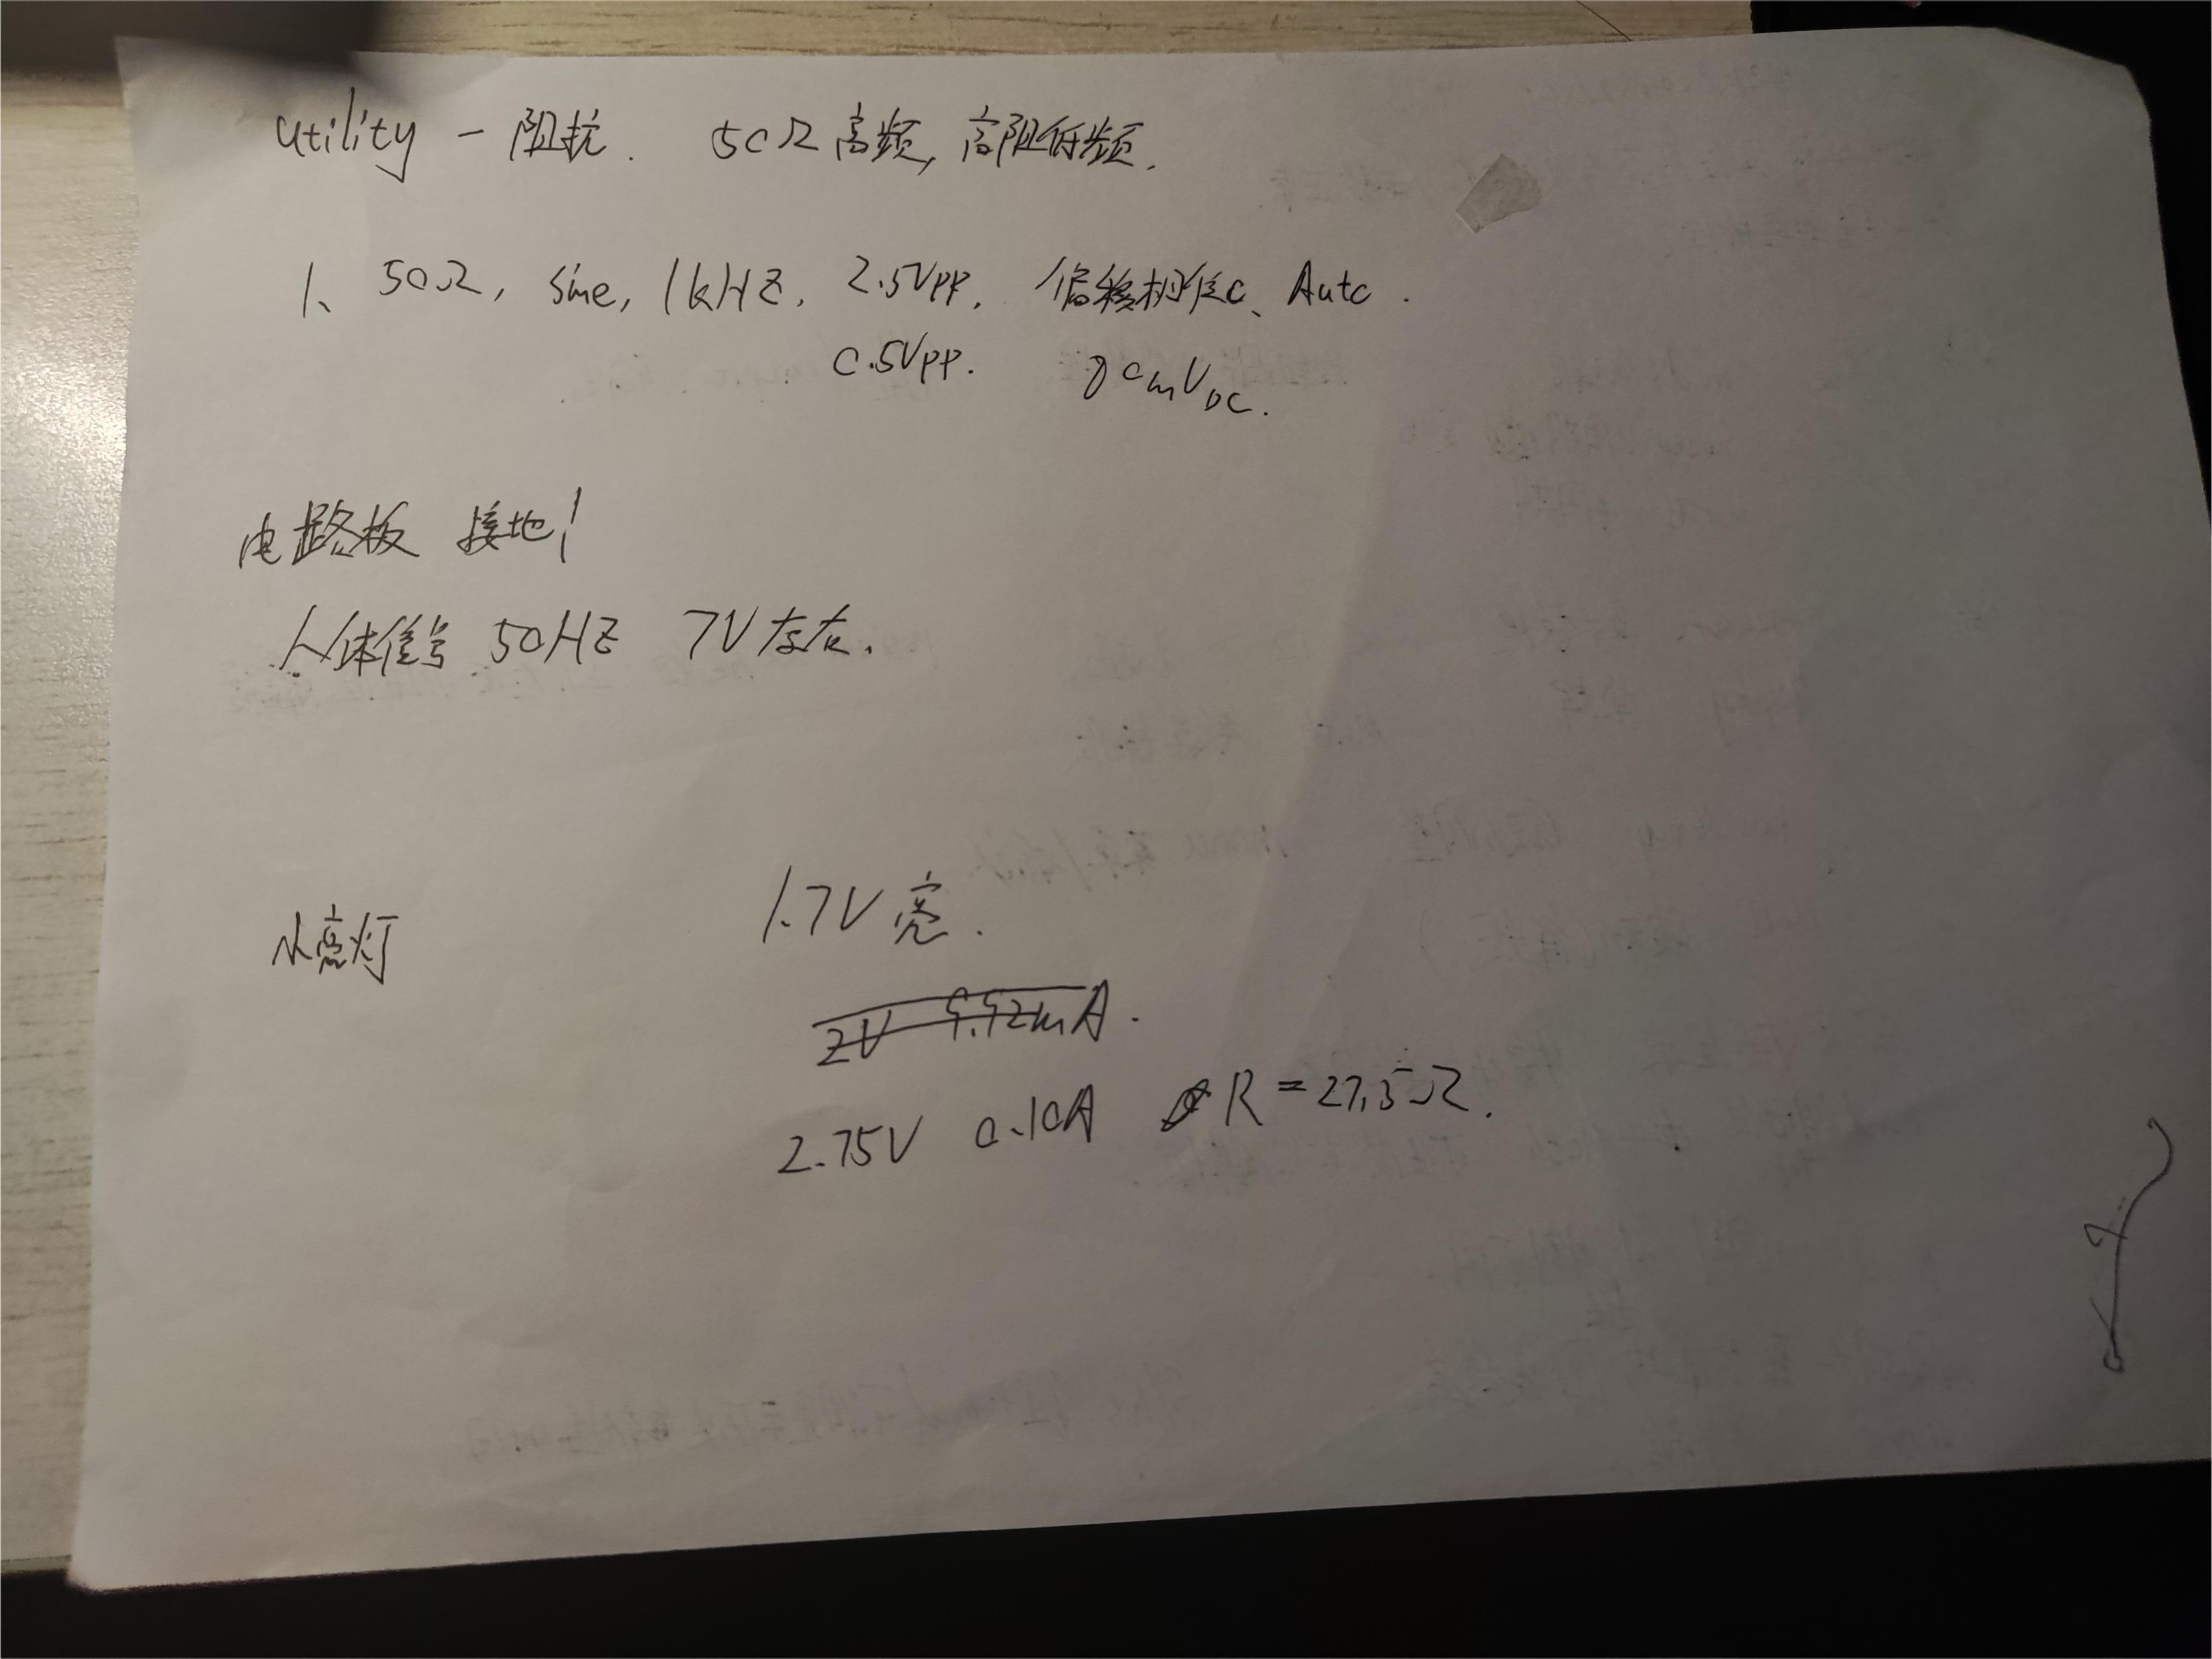
\includegraphics[width=8cm]{Fig/9.jpg}
        \caption{光学4F系统光路图}
    \end{figure}
    \item 在有第二个透镜和没有第二个透镜的情况下分别读取光屏上的像。
    \begin{figure}[H]
        \centering
        \begin{minipage}[t]{0.49\linewidth}
            \centering
            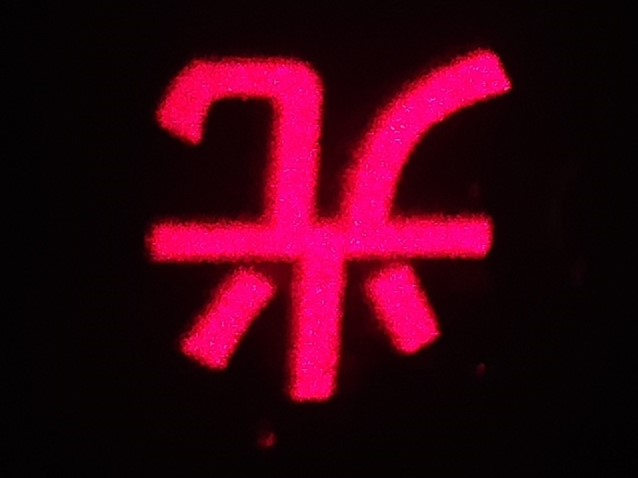
\includegraphics[width=7.5cm]{Fig/10-有透镜.jpg}
            \caption{有透镜}
        \end{minipage}
        \begin{minipage}[t]{0.49\linewidth}
            \centering
            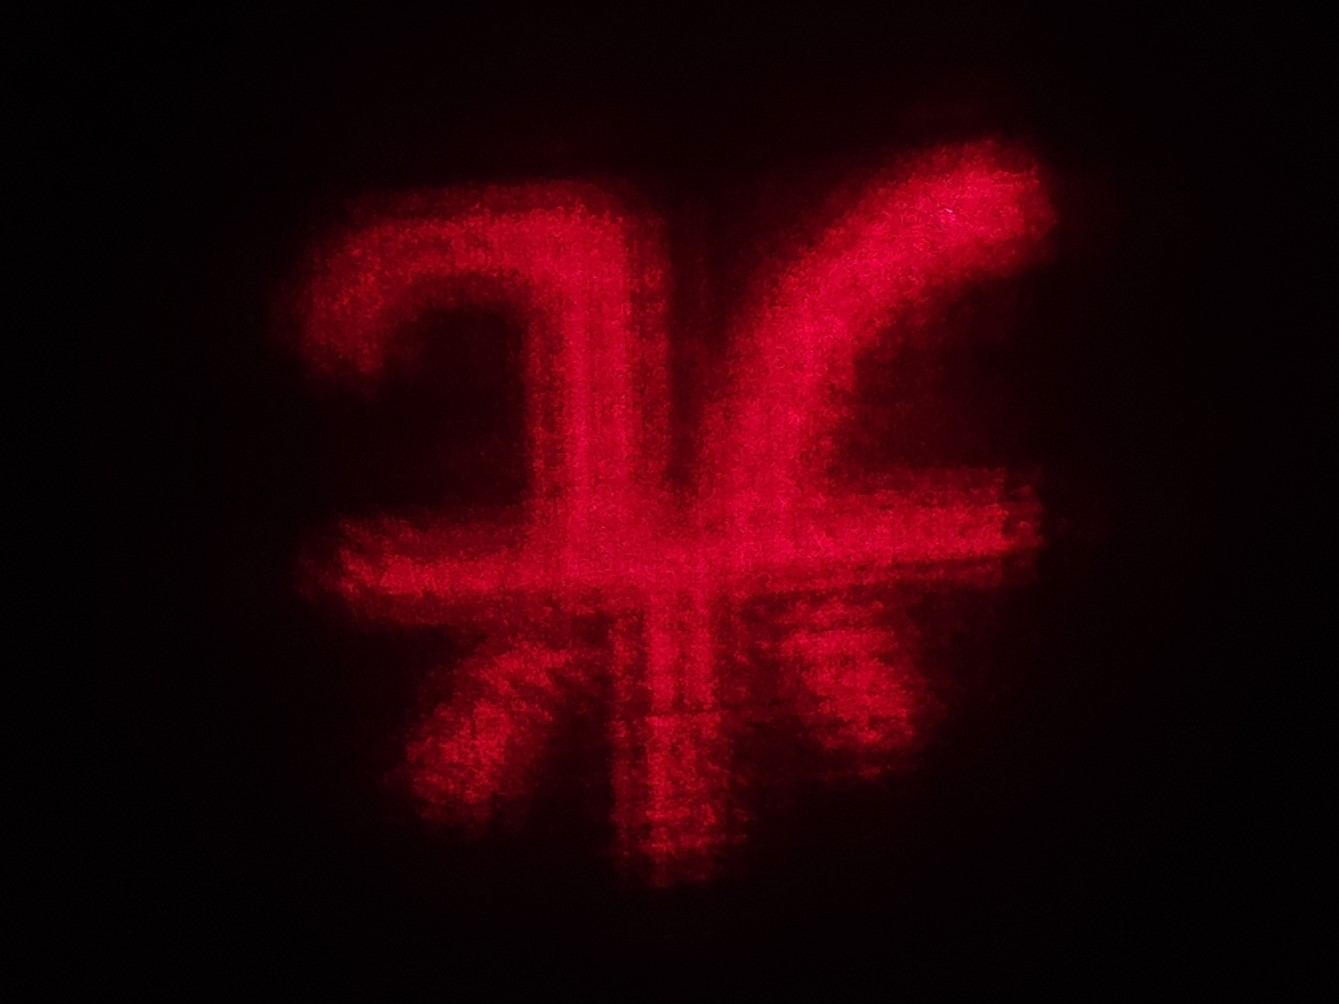
\includegraphics[width=7.5cm]{Fig/10-无透镜.jpg}
            \caption{无透镜}
        \end{minipage}
    \end{figure}
    \par \hspace*{2em}可以看到,有透镜时图像聚焦为原图像的倒像,无透镜时图像发生衍射产生衍射的叠加。
    \item 在纸上画出字,替换光栅字。在有第二个透镜和没有第二个透镜的情况下分别读取光屏上的像。
    \begin{figure}[H]
        \centering
        \begin{minipage}[t]{0.33\linewidth}
            \centering
            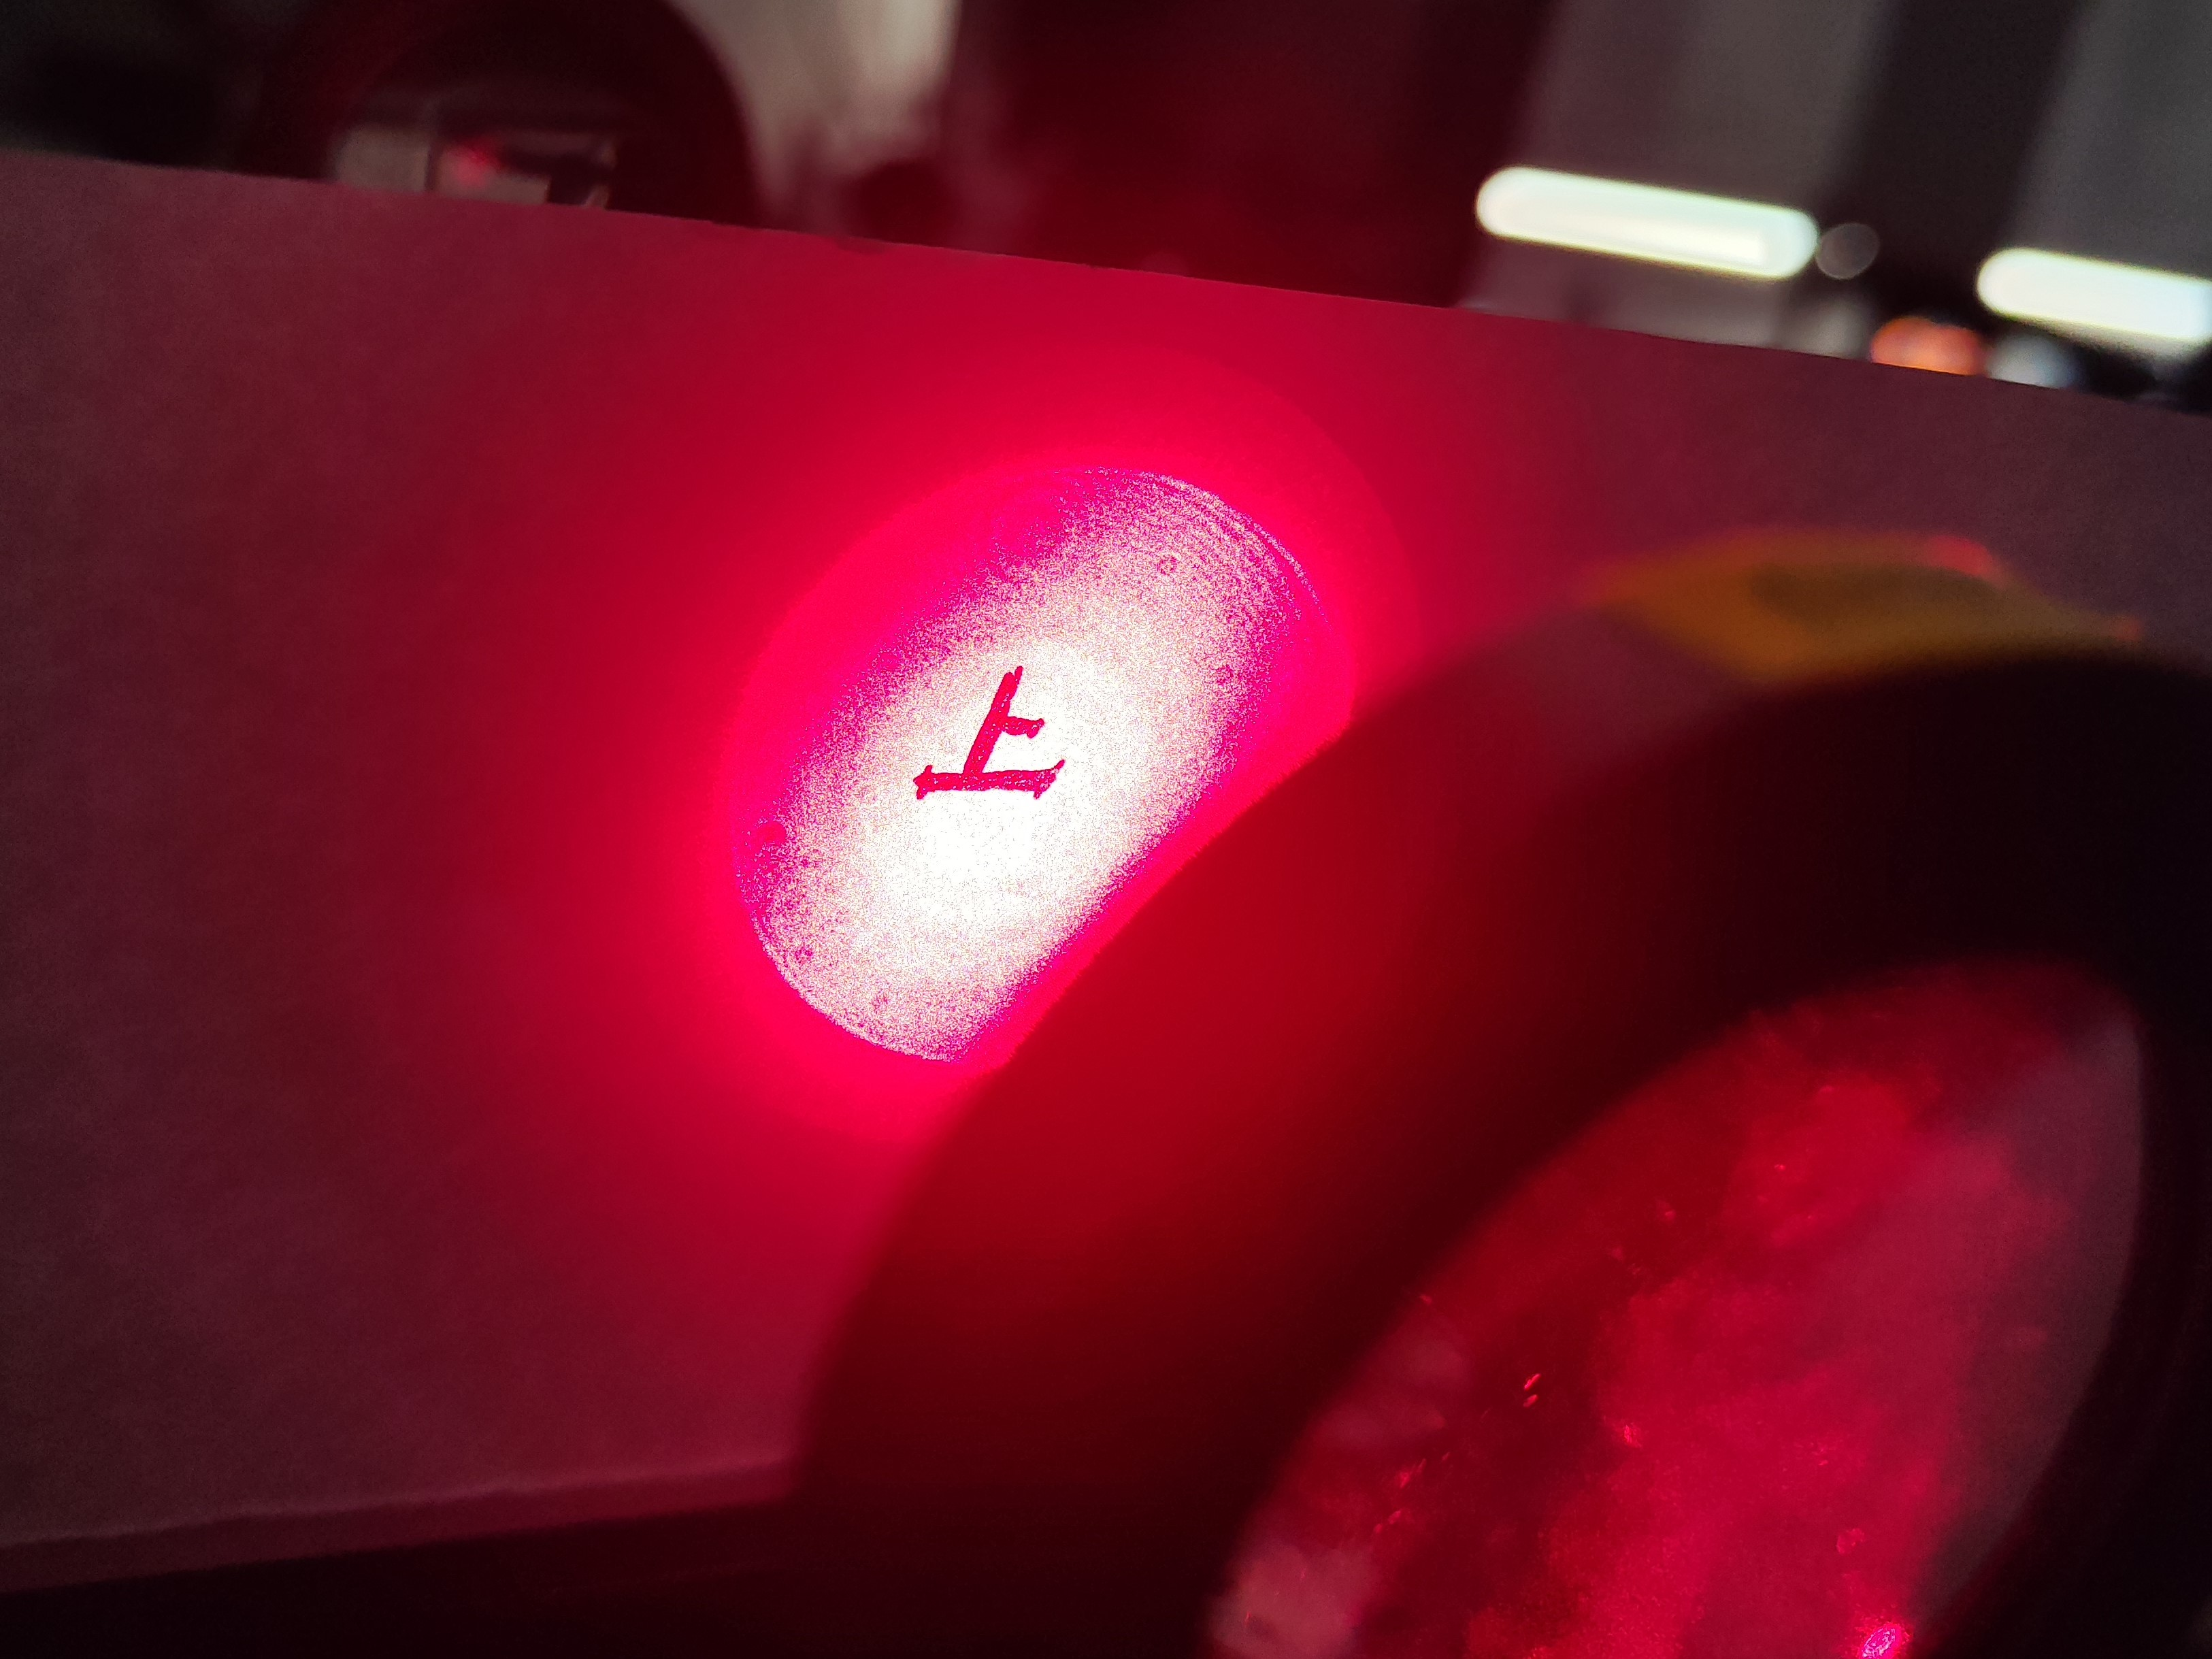
\includegraphics[width=5cm]{Fig/11-上字.jpg}
            \caption{所画字-上字}
        \end{minipage}
        \begin{minipage}[t]{0.33\linewidth}
            \centering
            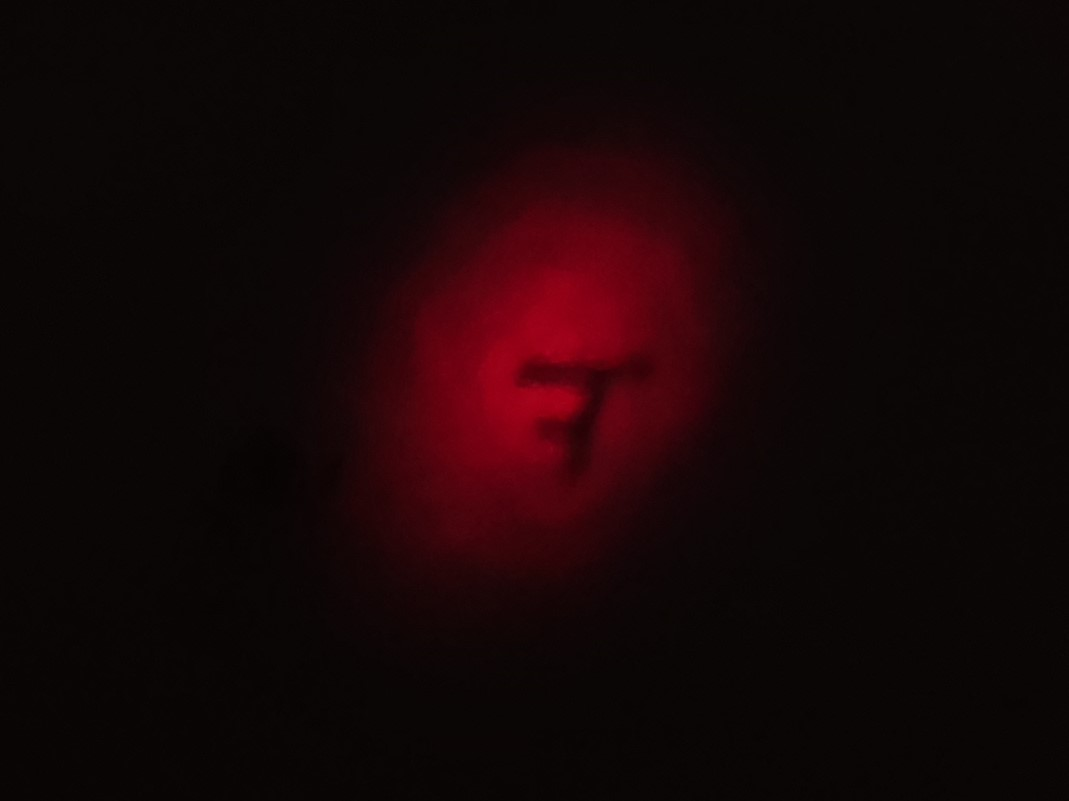
\includegraphics[width=5cm]{Fig/11-有透镜.jpg}
            \caption{有透镜}
        \end{minipage}
        \begin{minipage}[t]{0.33\linewidth}
            \centering
            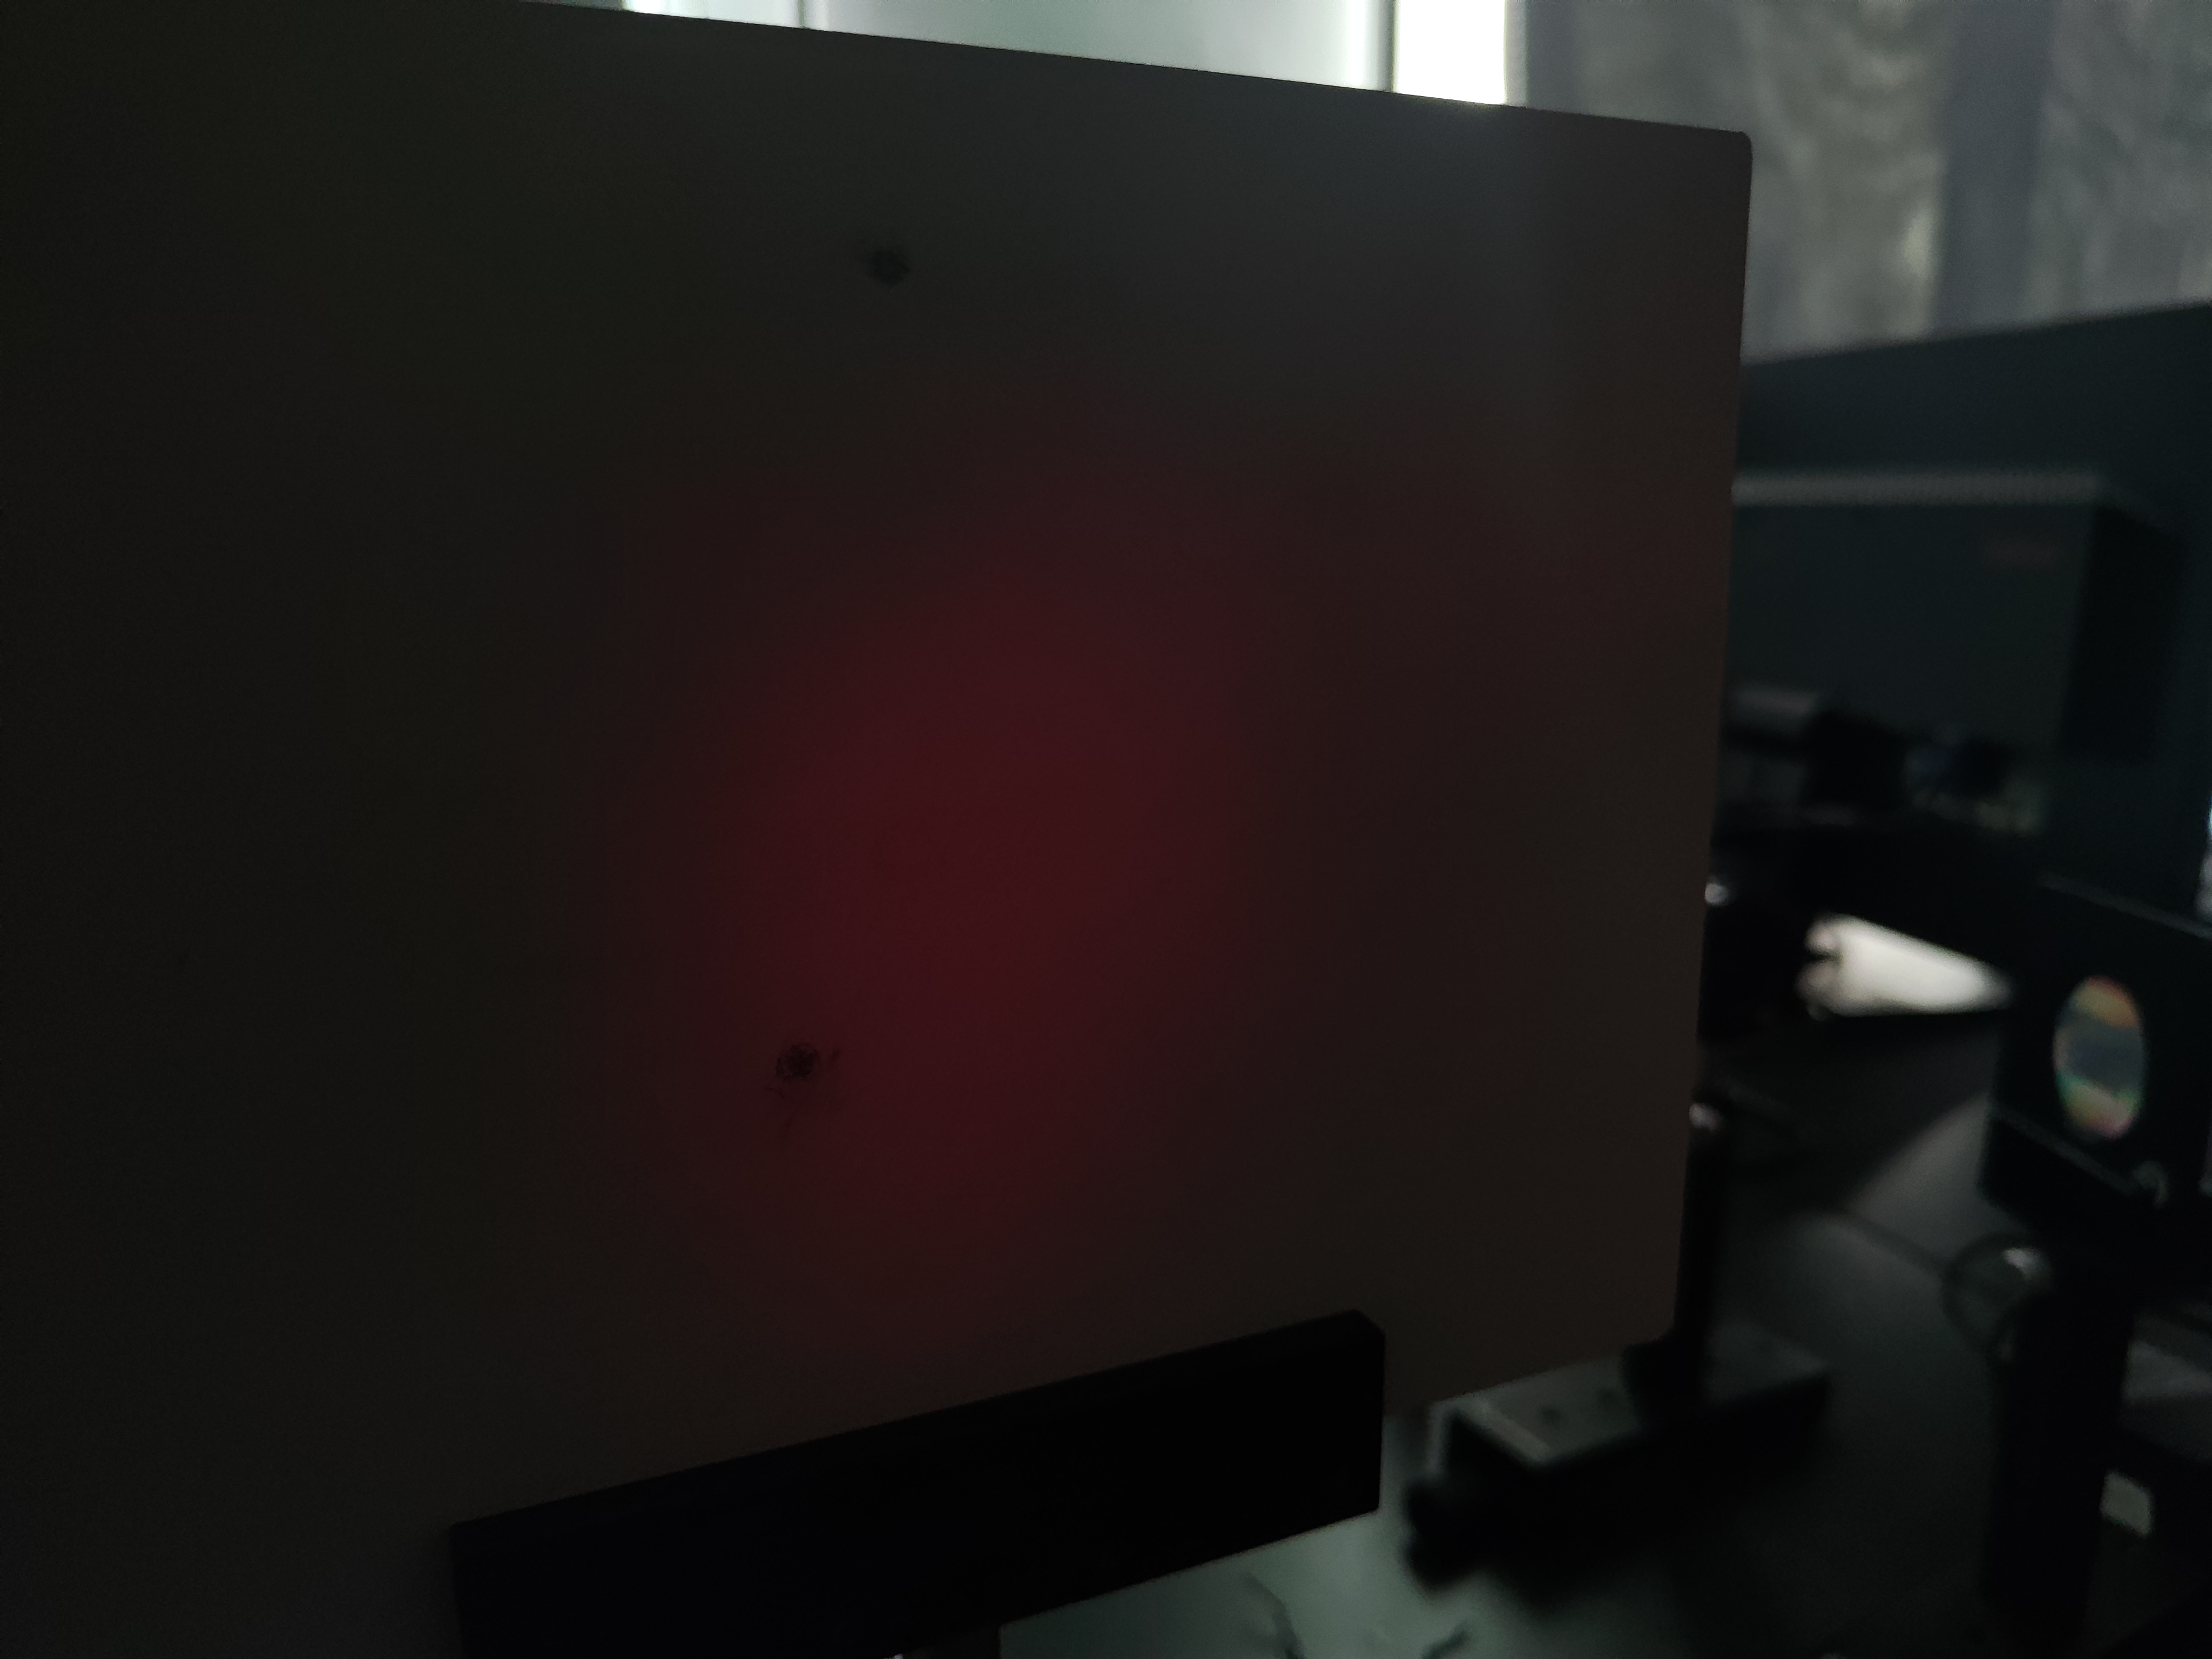
\includegraphics[width=5cm]{Fig/11-无透镜.jpg}
            \caption{无透镜}
        \end{minipage}
    \end{figure}
    \par \hspace*{2em} 可以看到,在有透镜时得到同时水平翻转和垂直翻转的像,在无透镜时由于衍射导致图像无法区分,得到大片暗红光。
    \par \hspace*{2em}这两组实验图像与阿贝成像的主要区别是:4F系统图像未经过扩散而变大,4F系统光屏在聚焦处才能看到清晰图像。
\end{enumerate}

\subsection{假彩色编码}
\noindent 实验过程:
\begin{enumerate}
    \item 如图和预习报告图搭建光路。调整光屏位置到聚焦点,得到清晰的像。
    \item 加入彩色滤片,得到彩色天安门城楼图像,天蓝楼红地绿。
    \begin{figure}[H]
        \centering
        \begin{minipage}[t]{0.49\linewidth}
            \centering
            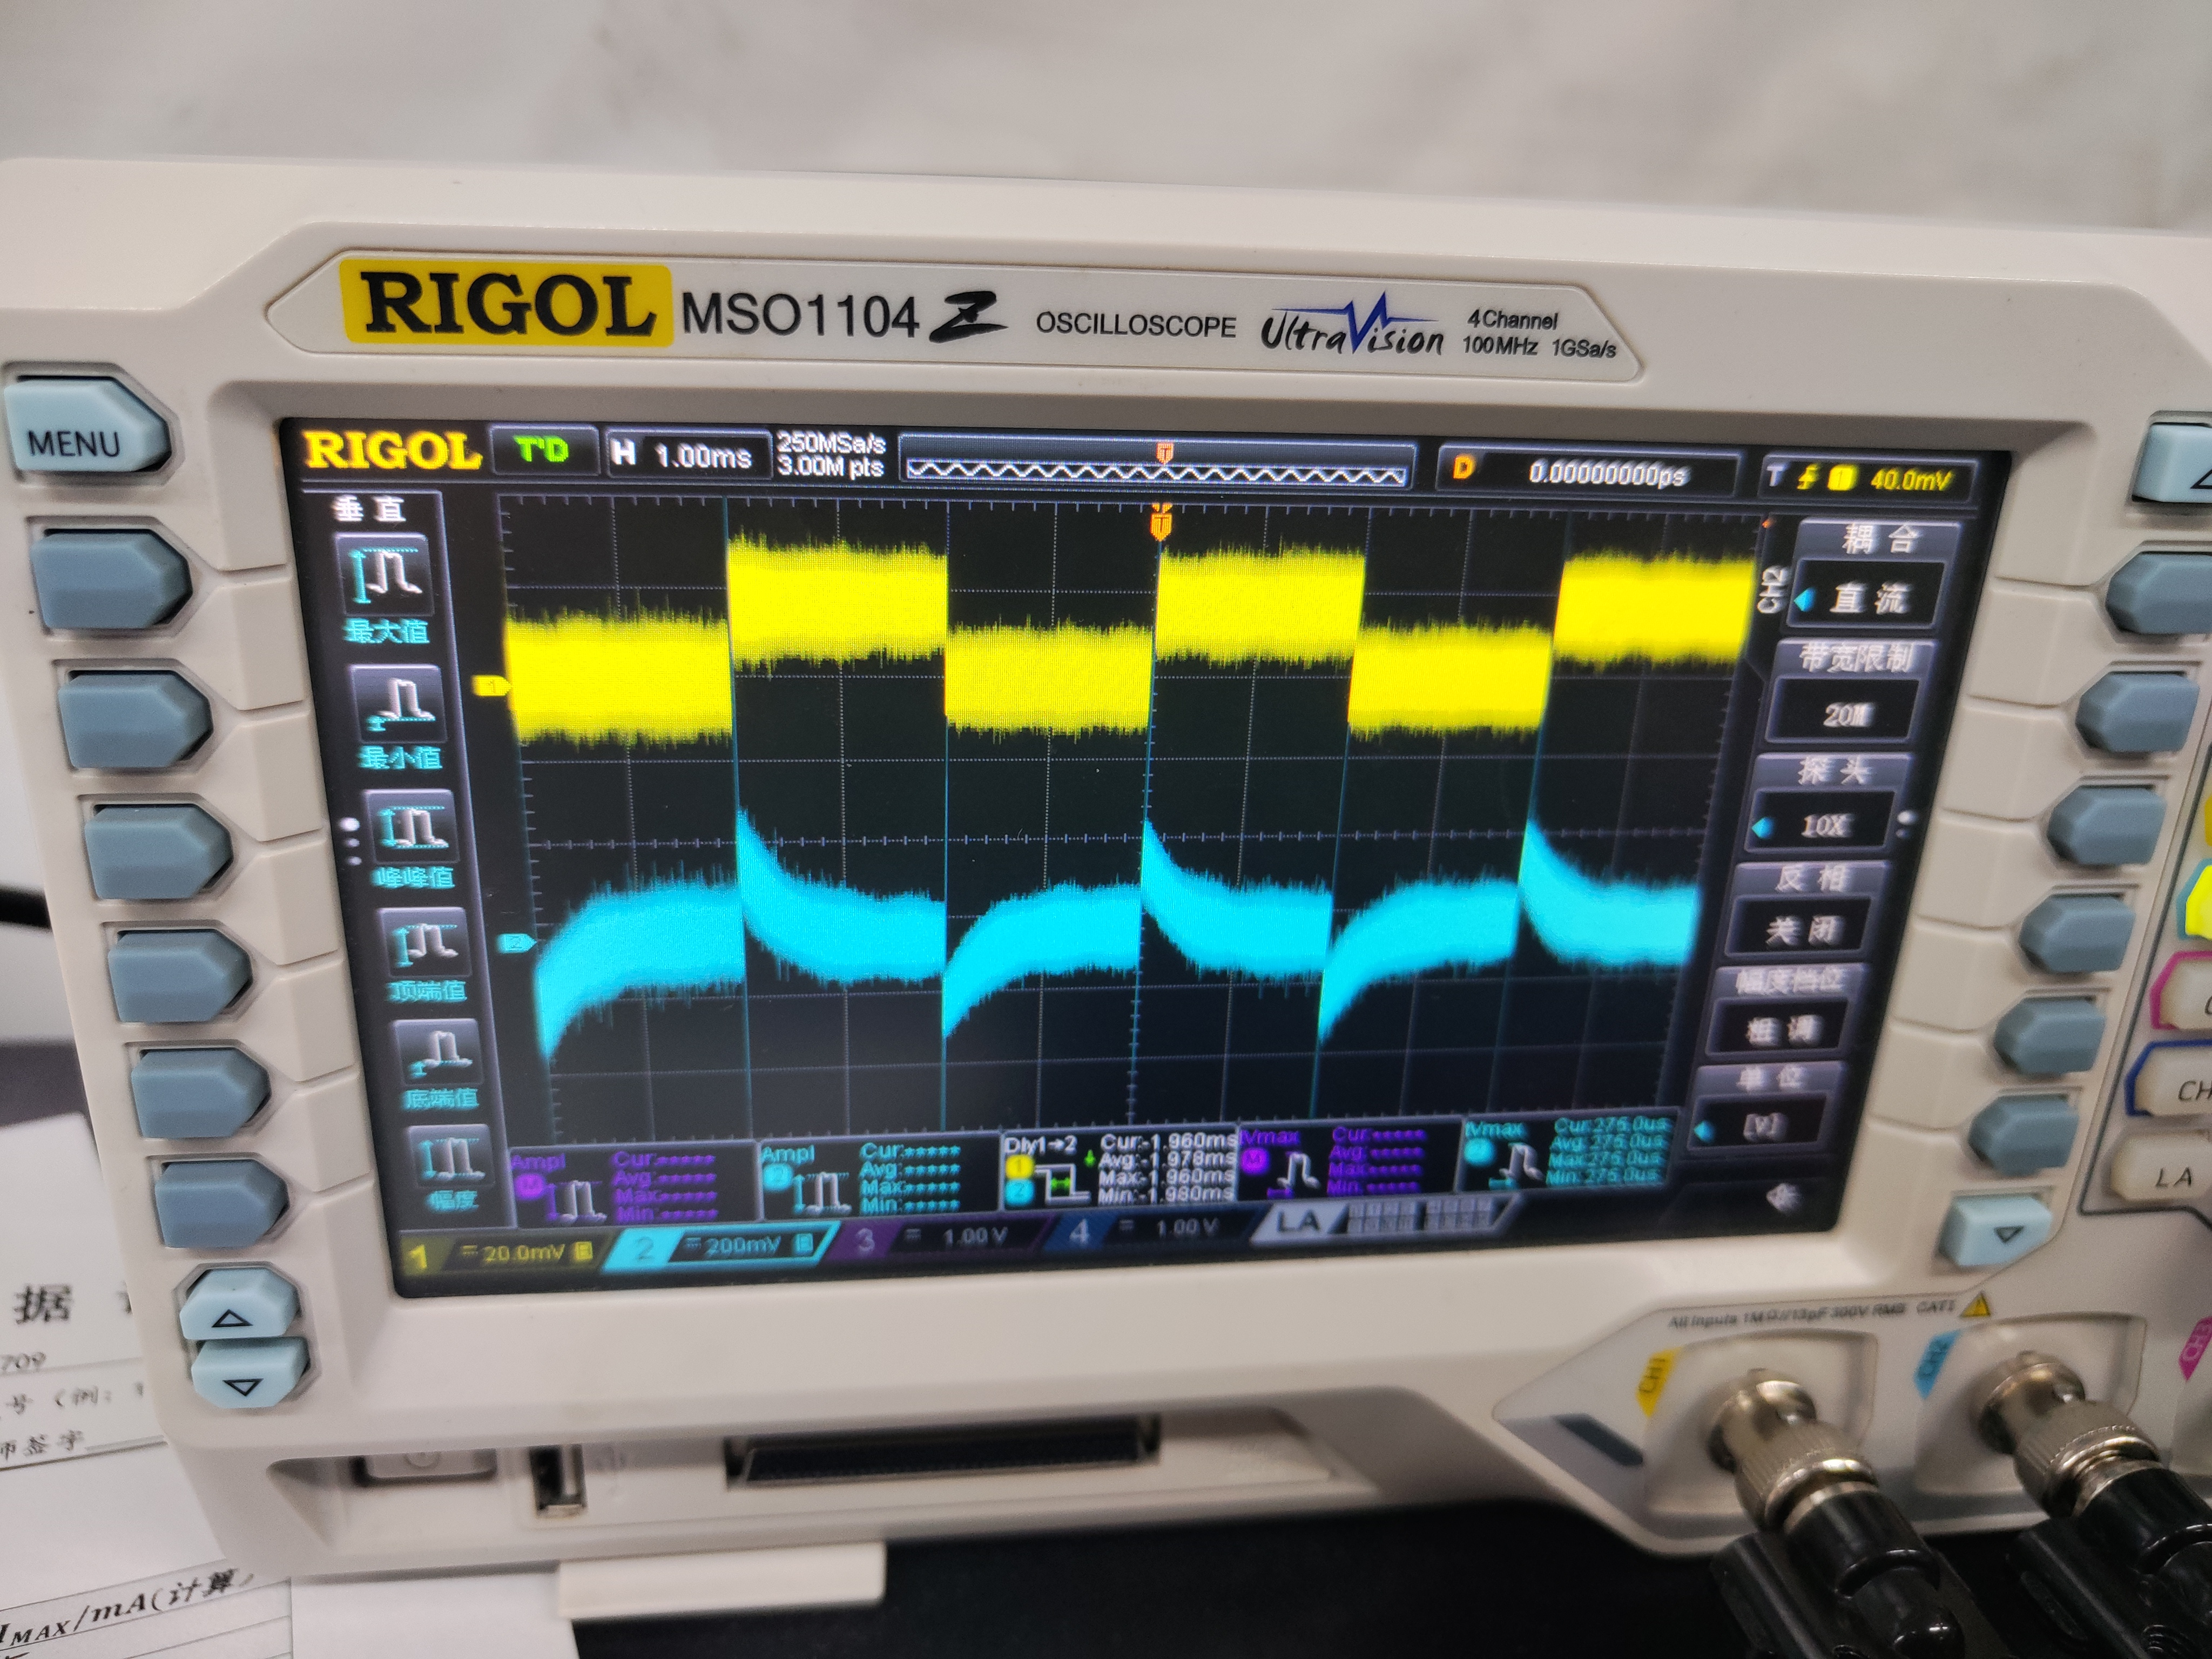
\includegraphics[width=7.5cm]{Fig/12.jpg}
            \caption{假彩色编码光路图}
        \end{minipage}
        \begin{minipage}[t]{0.49\linewidth}
            \centering
            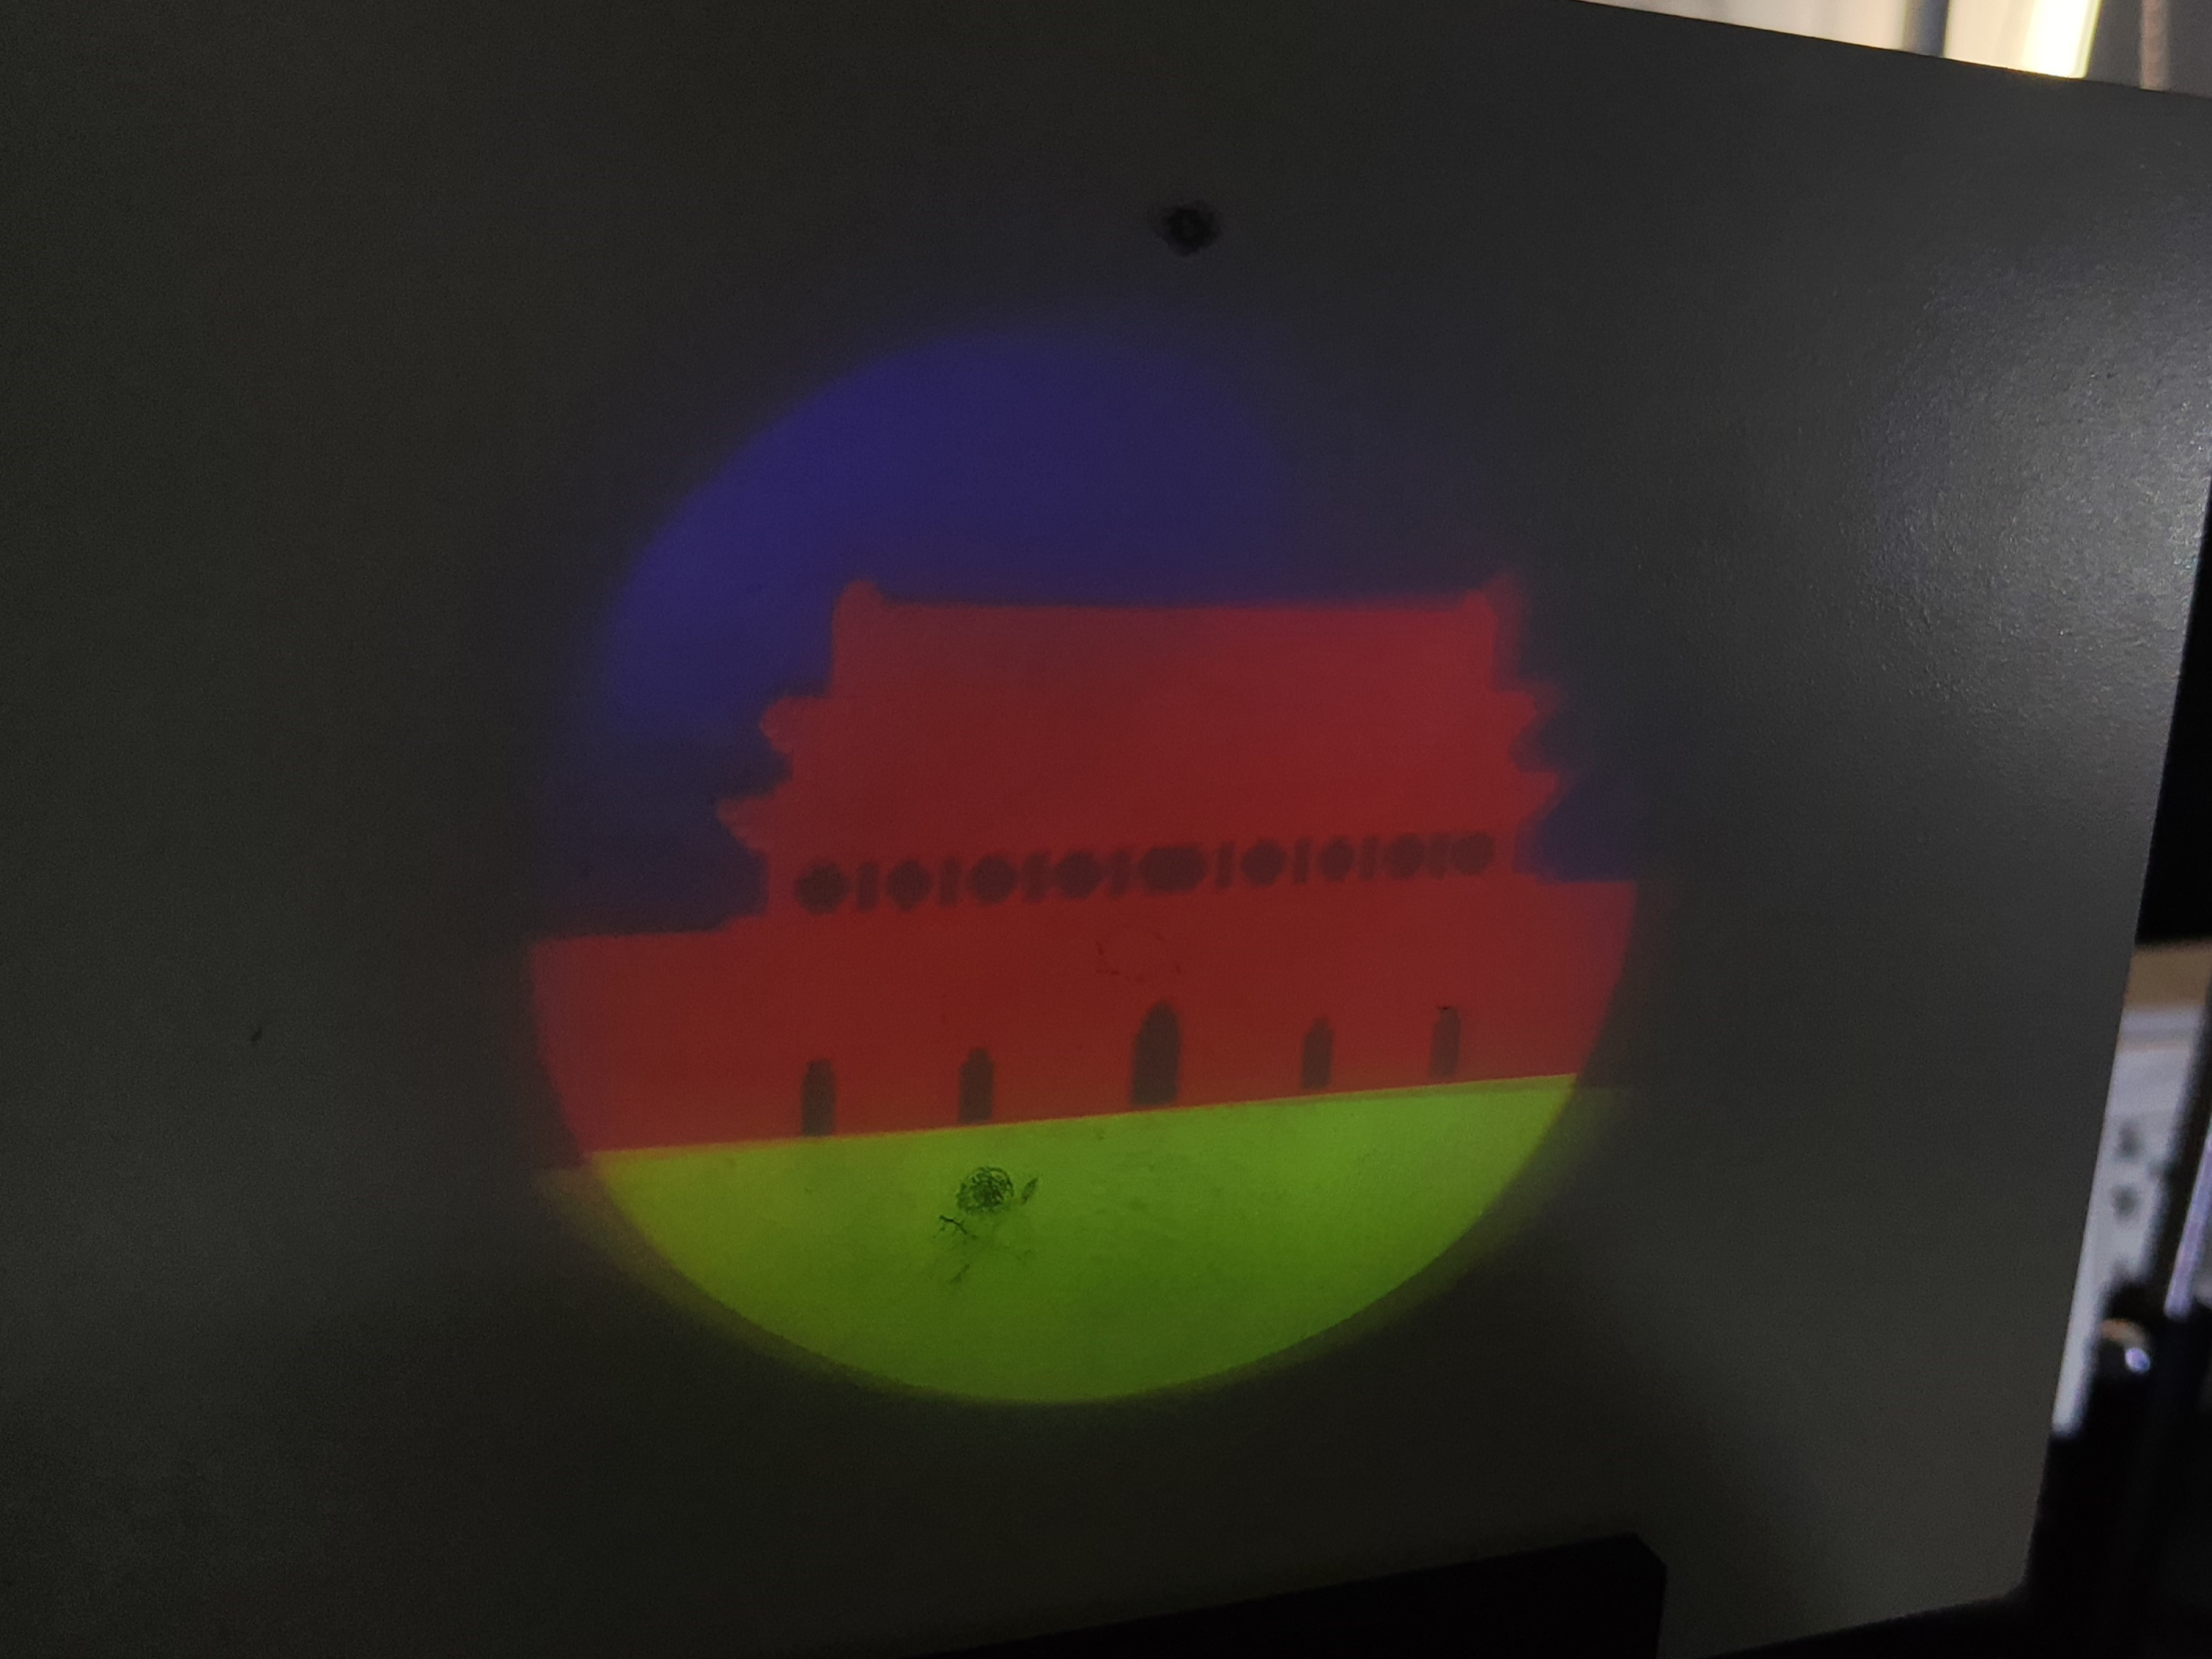
\includegraphics[width=7.5cm]{Fig/13.jpg}
            \caption{天安门城楼图像}
        \end{minipage}
    \end{figure}
    \item 根据频谱面,取水平绿,右斜红,左斜蓝,即与天安门光栅片对应部分垂直的方向,刻彩色滤纸,得到假彩色编码天安门城楼图像。
    \begin{figure}[H]
        \centering
        \begin{minipage}[t]{0.33\linewidth}
            \centering
            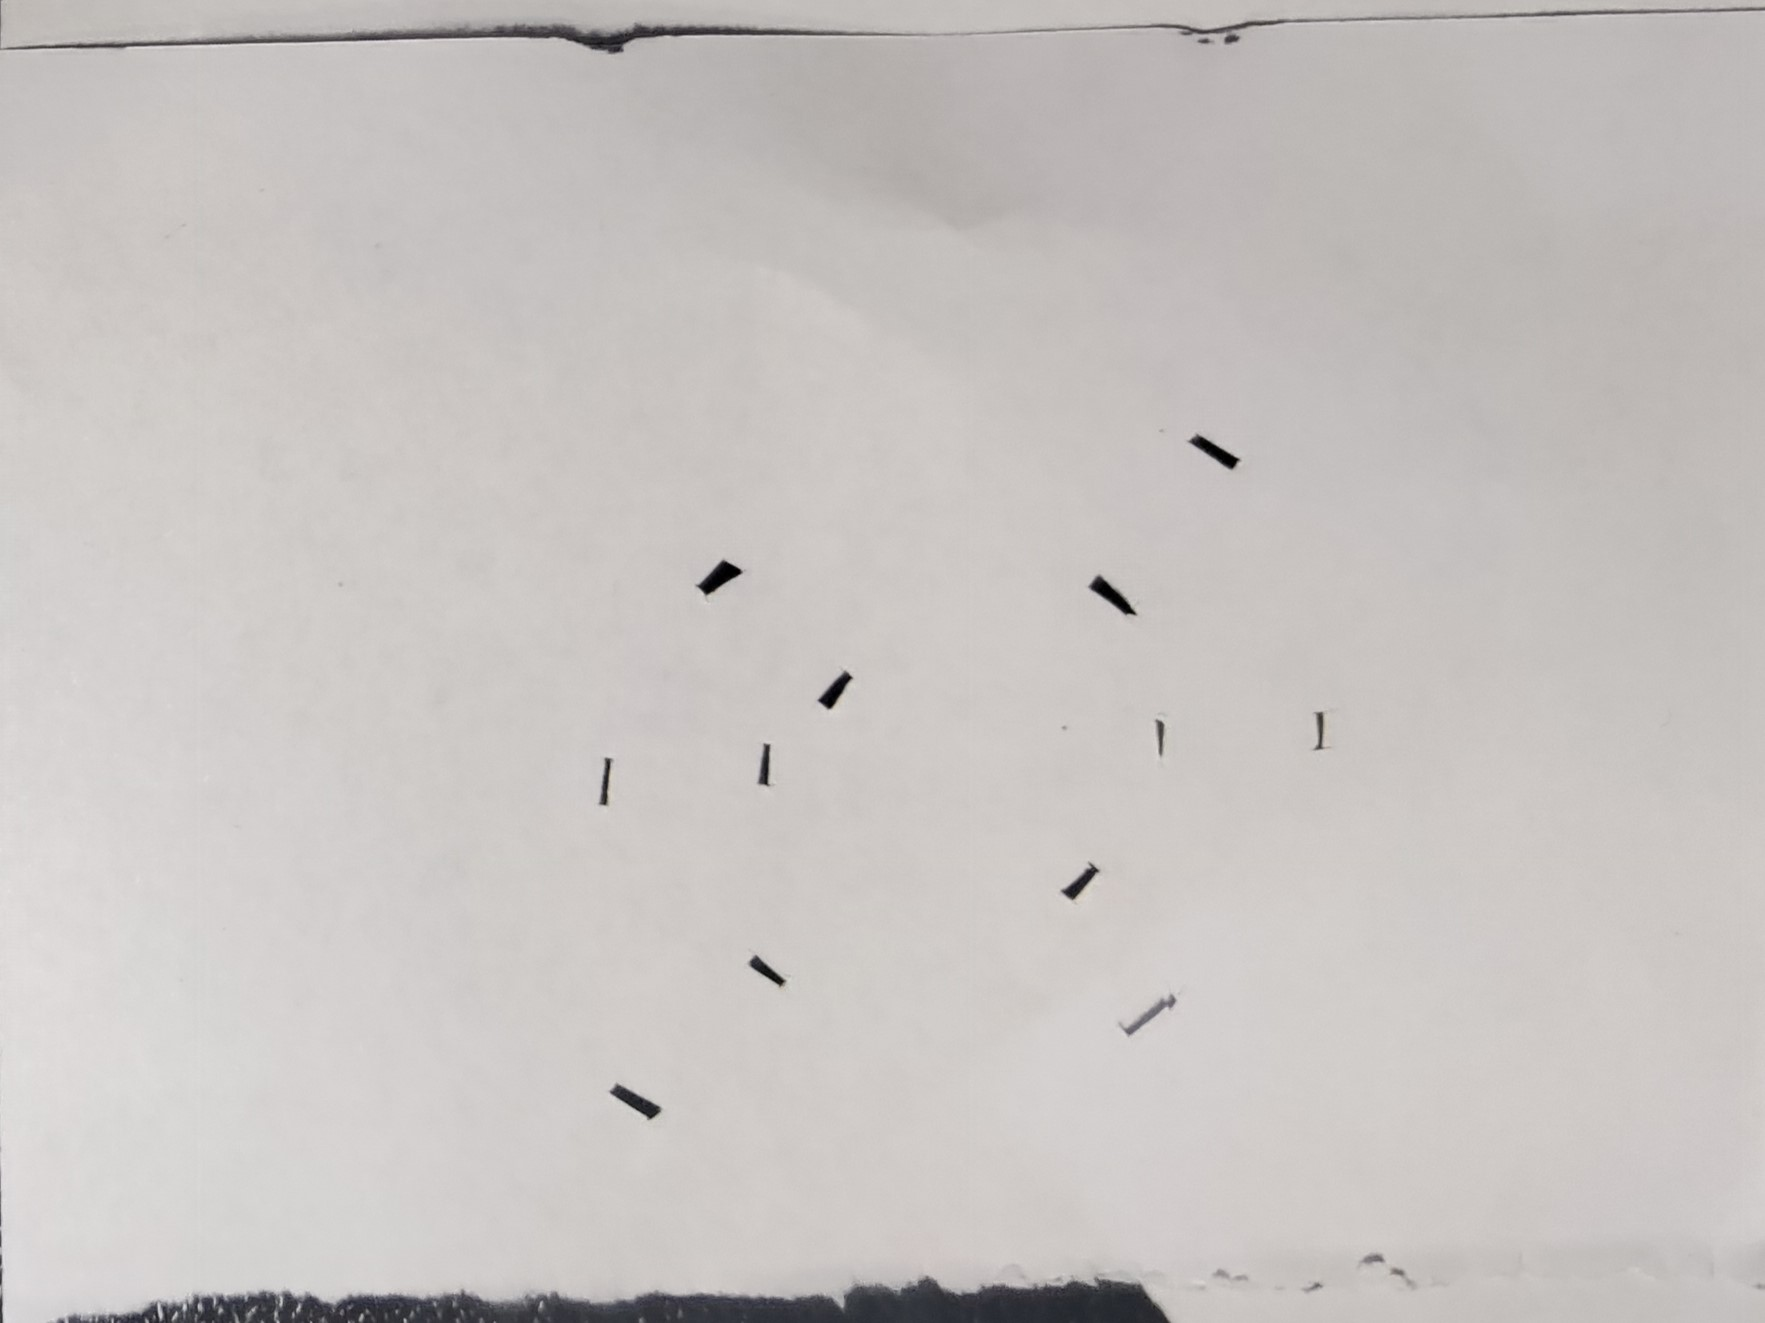
\includegraphics[width=5cm]{Fig/14.jpg}
            \caption{刻画滤纸}
        \end{minipage}
        \begin{minipage}[t]{0.33\linewidth}
            \centering
            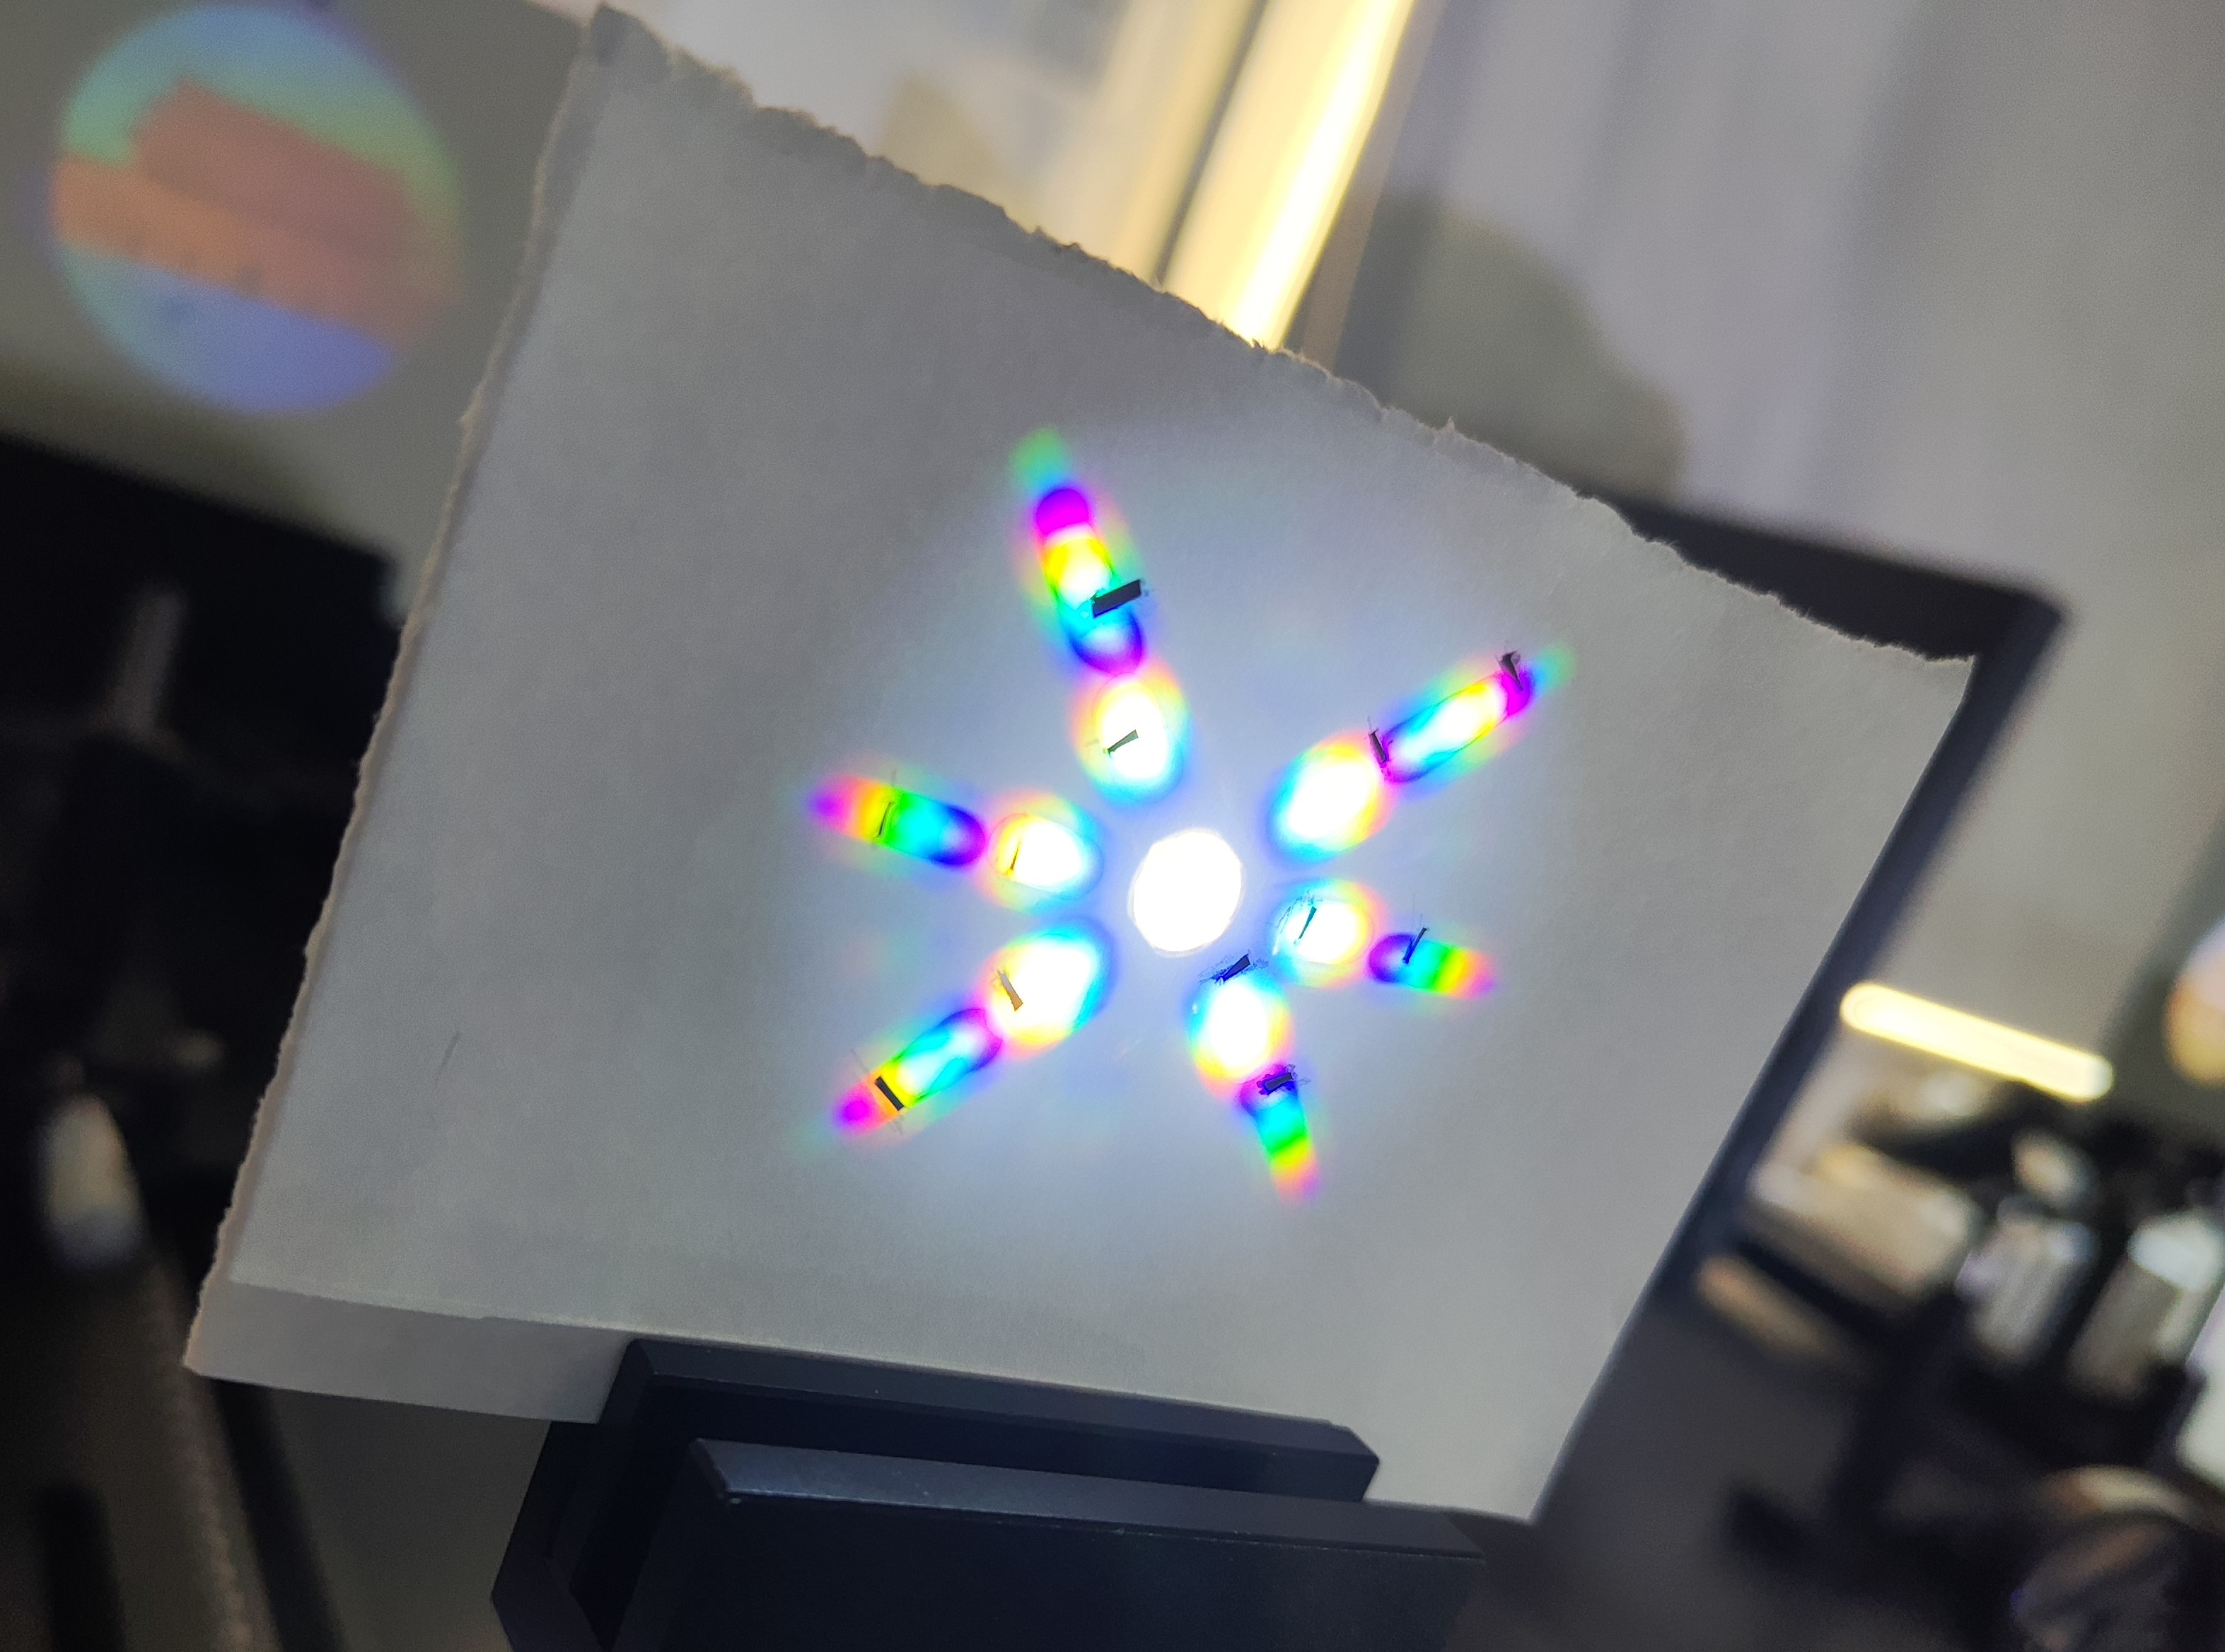
\includegraphics[width=5cm]{Fig/15.jpg}
            \caption{频谱面}
        \end{minipage}
        \begin{minipage}[t]{0.33\linewidth}
            \centering
            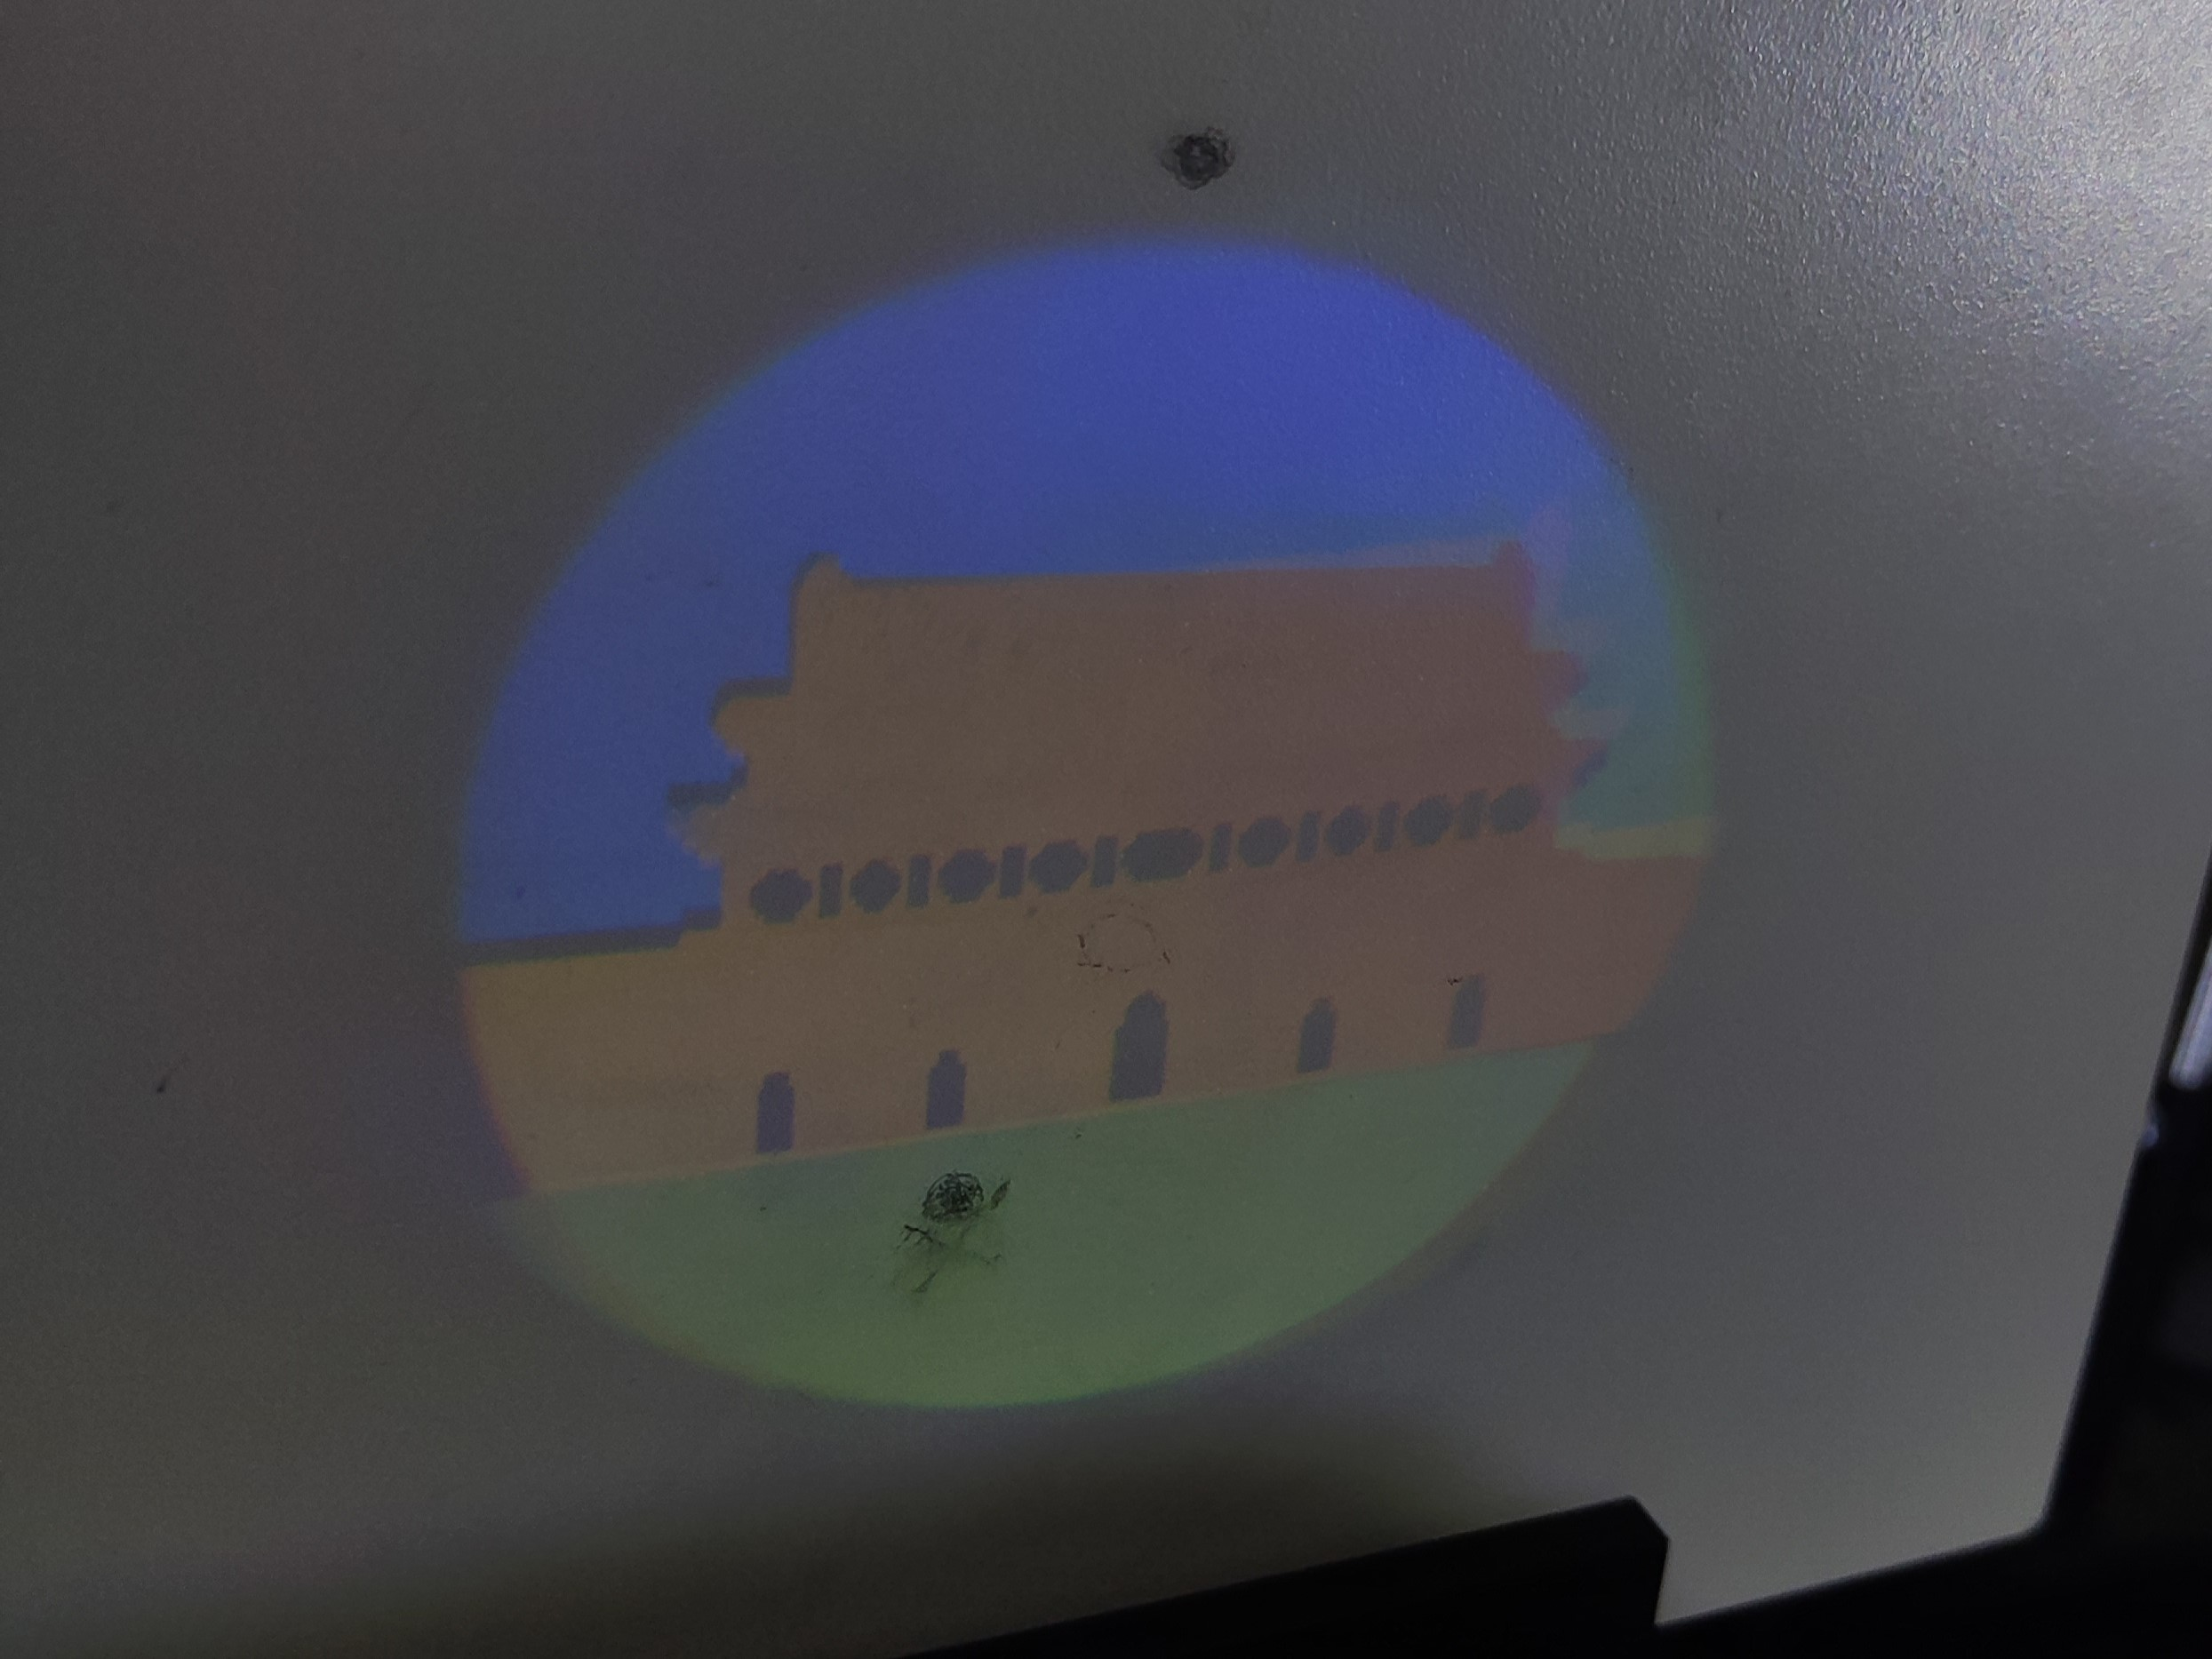
\includegraphics[width=5cm]{Fig/16.jpg}
            \caption{假彩色编码天安门城楼图像}
        \end{minipage}
    \end{figure} 
    \par \hspace*{2em}可以看到,频谱面每一个条带内侧蓝色,外侧红色,颜色均匀变化。波长越长,衍射图谱越靠外(条纹间距离越大)。根据此规律在每个方向取四个对应颜色区域刻掉得到假彩色编码滤纸,所得天安门城楼图像大致满足天蓝楼红地绿的要求。
    \par \hspace*{2em}现在所得图像的天安门城楼门洞是黑色的,若想让门洞变亮,则需要将中心亮斑的区域刻掉。

\end{enumerate}

\subsection{光栅衍射测量光栅常数实验}
\noindent 实验过程:
\begin{enumerate}
    \item 如图搭建光路,根据光斑位置调整光屏至合适距离。
    \item 测量光栅片到光屏的距离L和光斑间距$\Delta x$。
    \begin{figure}[H]
        \centering
        \includegraphics[width=8cm]{Fig/17.jpg}
        \caption{测量光栅常数光路图}
    \end{figure}
    \item 测量结果为:$L=60cm,\Delta x =4cm$。由$d=\frac{\lambda}{\sin \theta}=\lambda\frac{\sqrt{L^2+{\Delta x}^2}}{\Delta x}=9.8\times 10^{-6}(m)$,光栅线密度$\frac{1}{d}=102(mm^{-1})\approx 100(mm^{-1})$。所以我所拿到的光栅,线密度100每毫米。

\end{enumerate}

\subsection{光栅光谱仪测光谱实验}
\noindent 实验过程:
\begin{enumerate}
    \item 搭建光路,将光纤头紧贴白色LED。
    %这里缺图
    \item 打开软件,得到光谱图,并用origin处理。
    \begin{figure}[H]
        \centering
        \begin{minipage}[t]{0.55\linewidth}
            \centering
            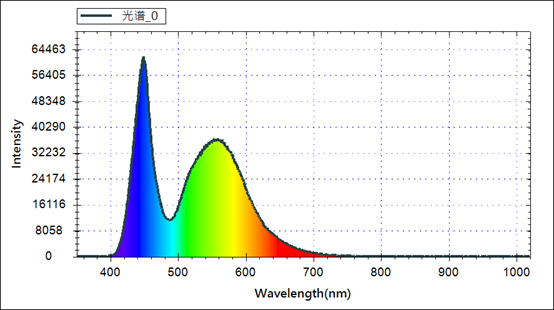
\includegraphics[width=8cm]{Fig/18.png}
            \caption{白光光谱}
        \end{minipage}
        \begin{minipage}[t]{0.44\linewidth}
            \centering
            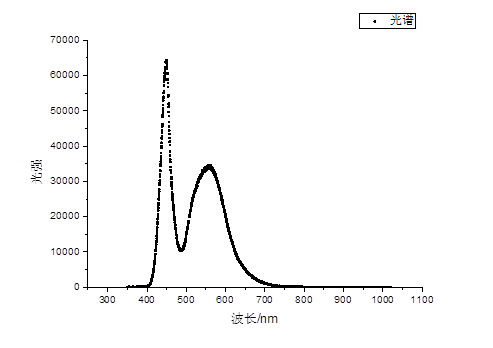
\includegraphics[width=6.5cm]{Fig/19.png}
            \caption{处理白光光谱}
        \end{minipage}
    \end{figure}
    \item 加入红绿蓝彩色滤纸,分别得到光谱图,并用origin处理。
    \begin{figure}[H]
        \centering
        \begin{minipage}[t]{0.55\linewidth}
            \centering
            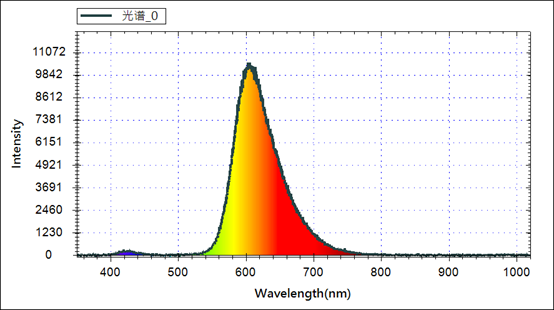
\includegraphics[width=8cm]{Fig/20-红.png}
            \caption{红光光谱}
        \end{minipage}
        \begin{minipage}[t]{0.44\linewidth}
            \centering
            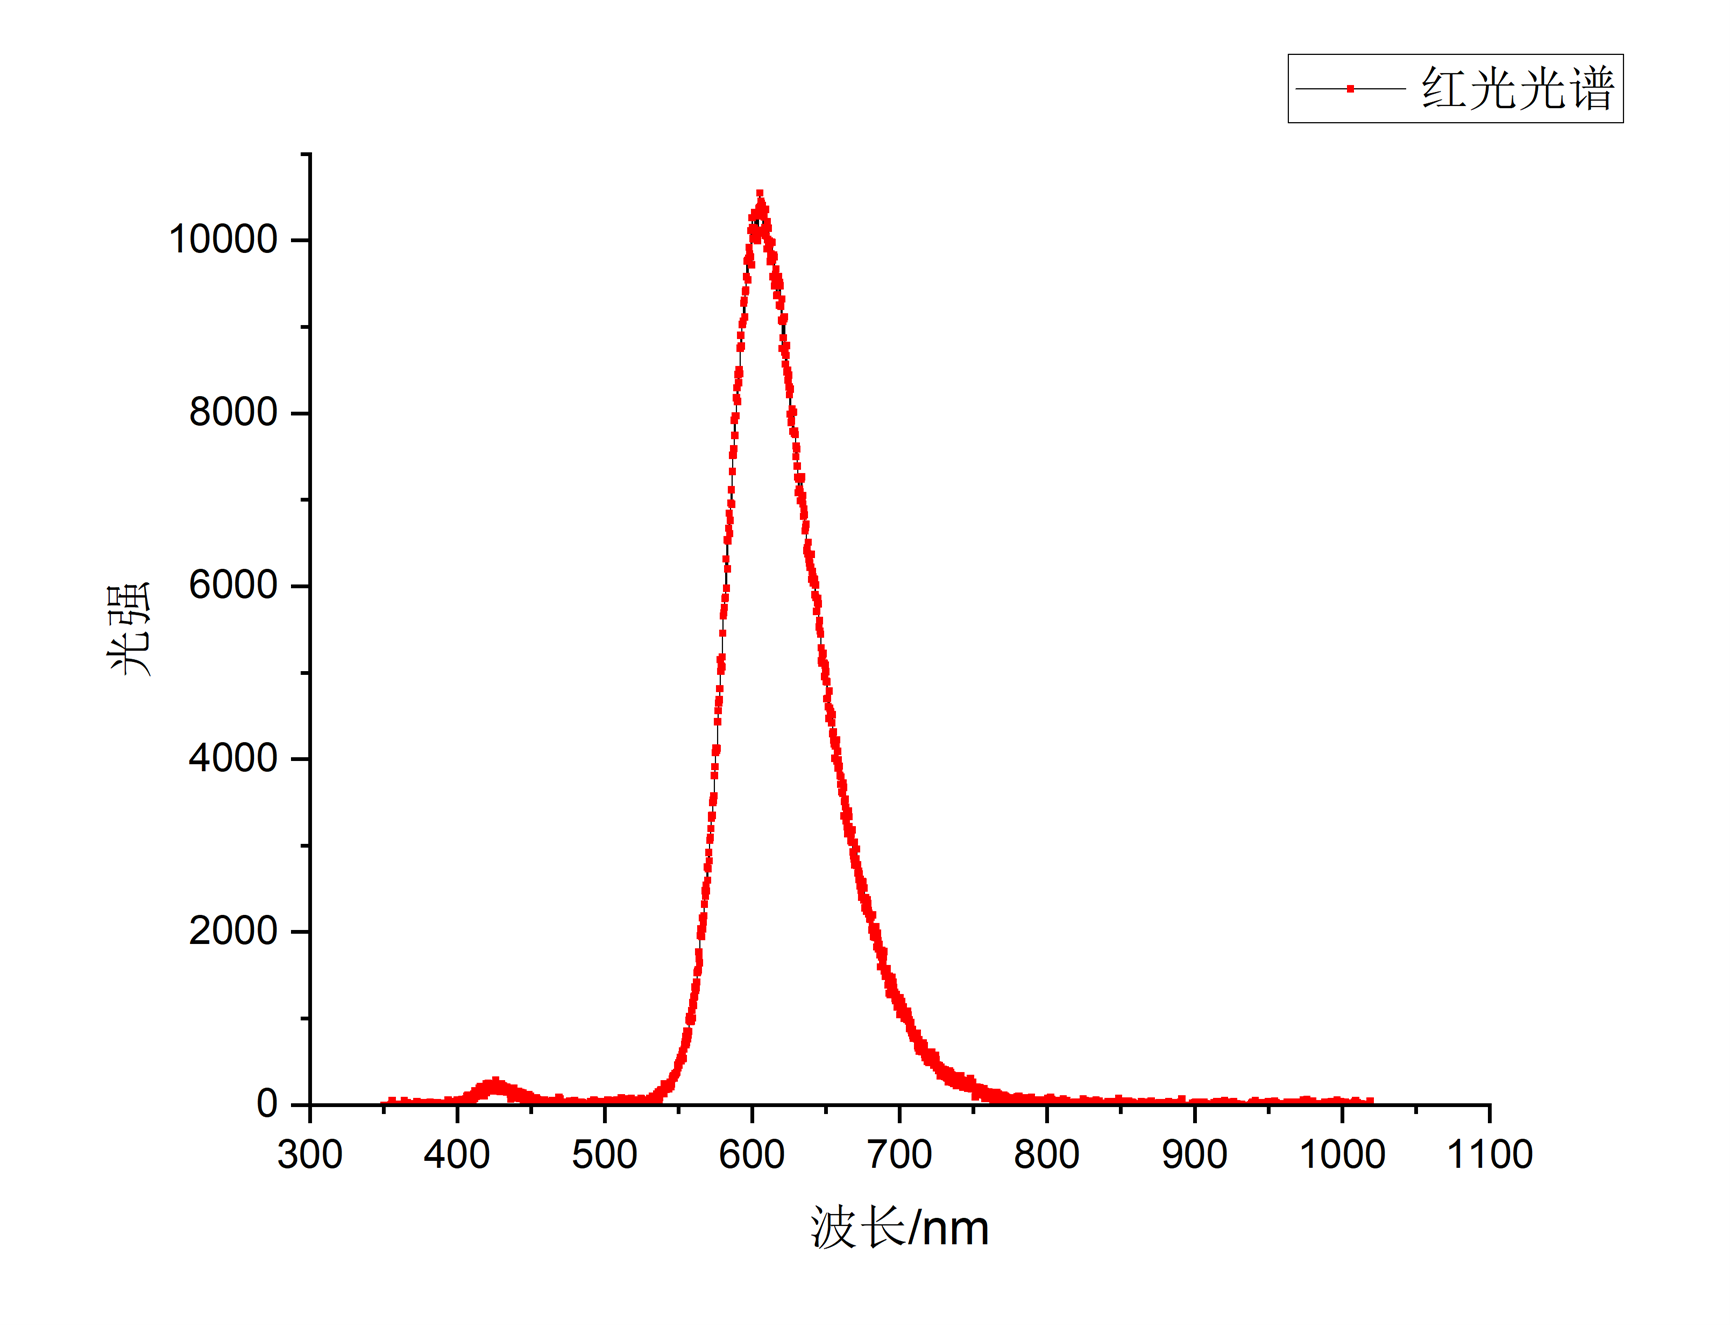
\includegraphics[width=6.5cm]{Fig/21-红.png}
            \caption{处理红光光谱}
        \end{minipage}
    \end{figure}
    \begin{figure}[H]
        \centering
        \begin{minipage}[t]{0.55\linewidth}
            \centering
            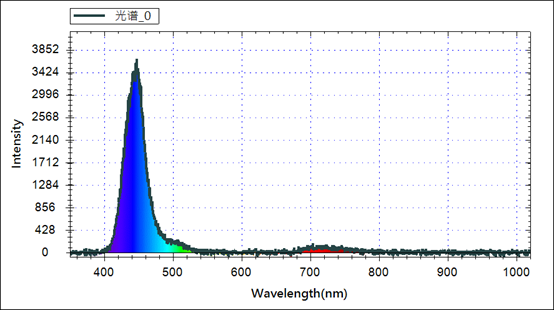
\includegraphics[width=8cm]{Fig/22-蓝.png}
            \caption{蓝光光谱}
        \end{minipage}
        \begin{minipage}[t]{0.44\linewidth}
            \centering
            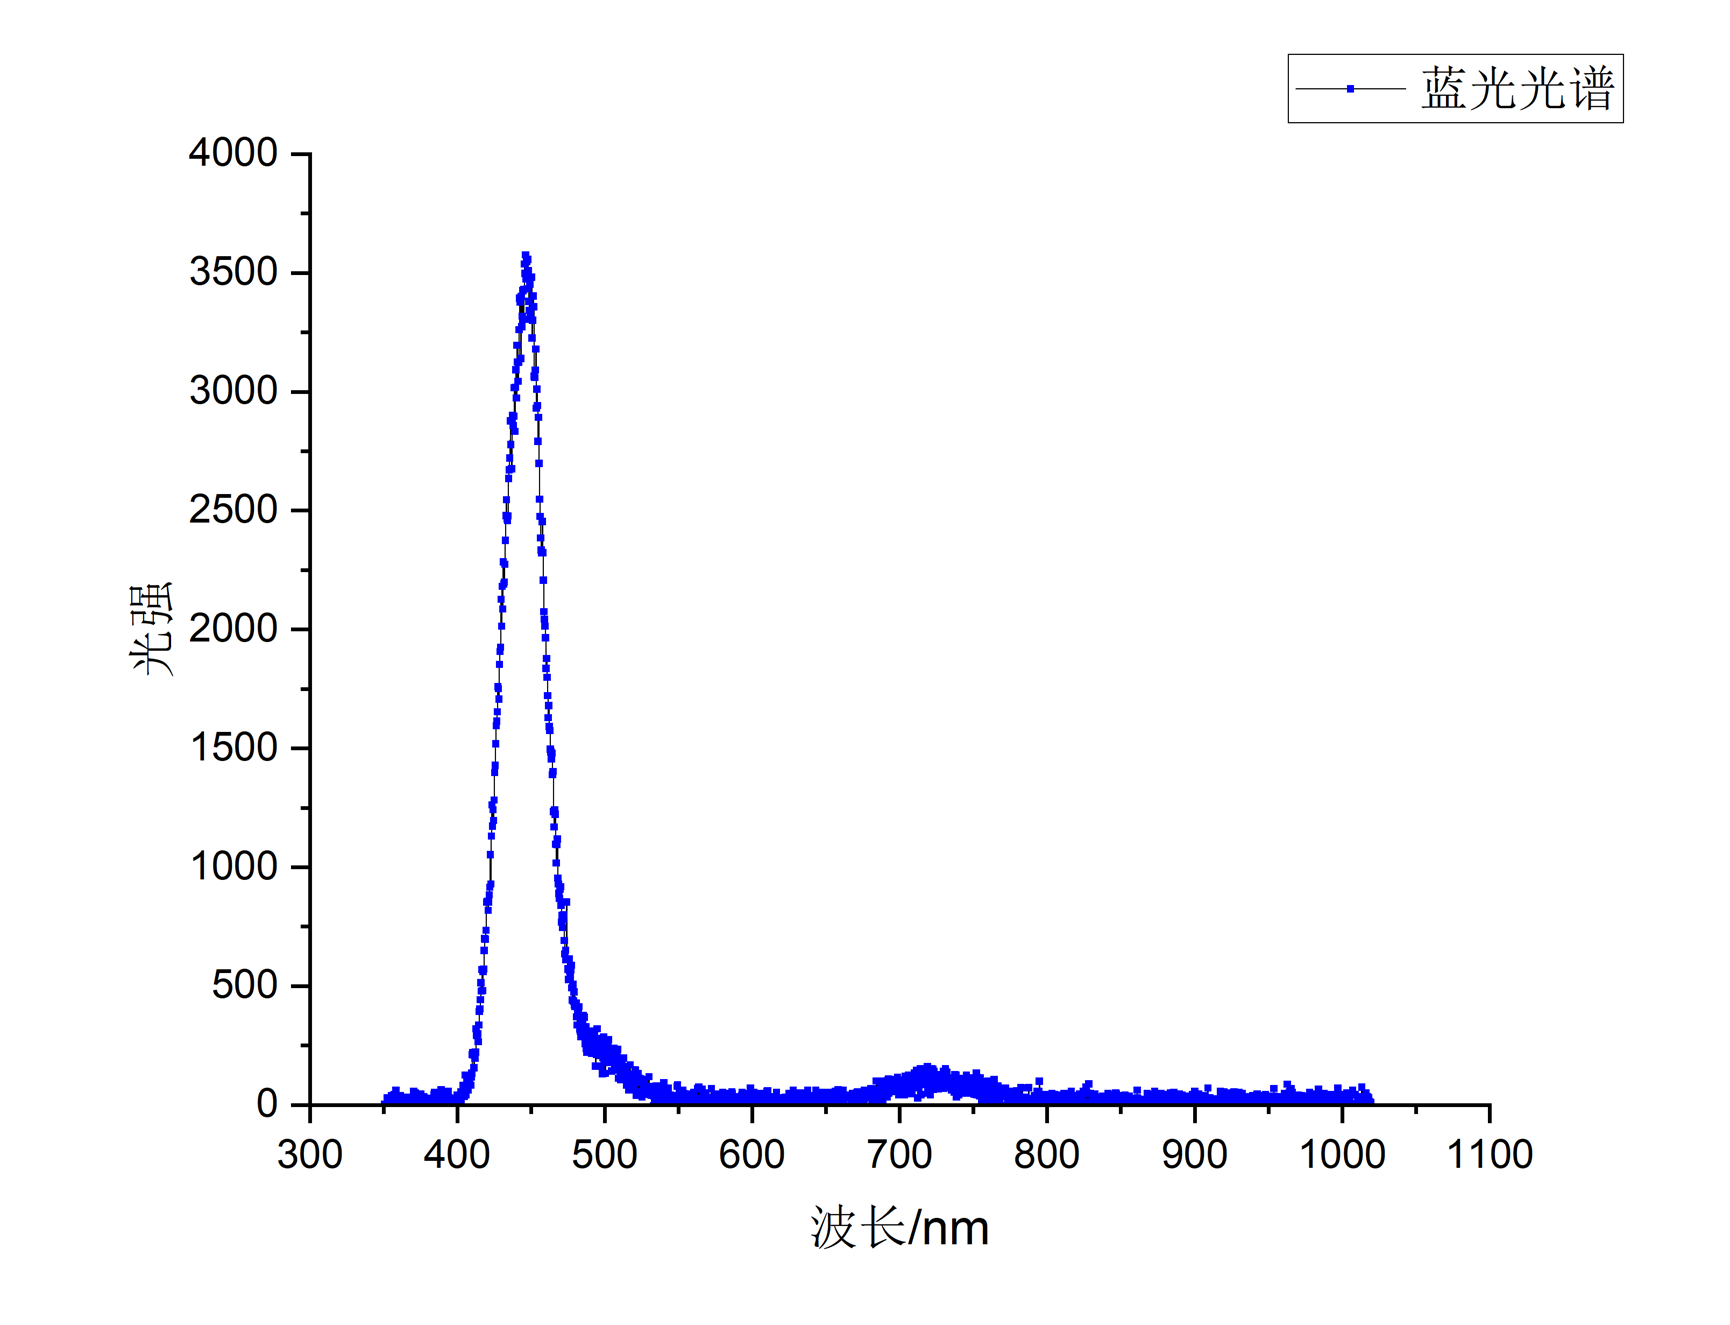
\includegraphics[width=6.5cm]{Fig/23-蓝.png}
            \caption{处理蓝光光谱}
        \end{minipage}
    \end{figure}

    \begin{figure}[H]
        \centering
        \begin{minipage}[t]{0.55\linewidth}
            \centering
            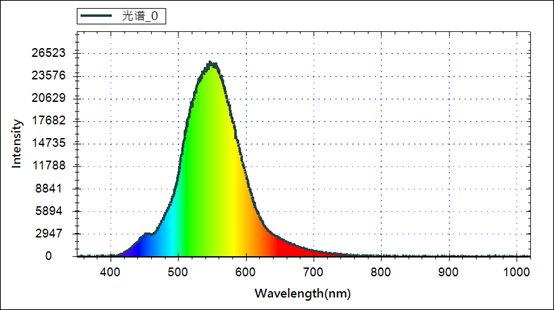
\includegraphics[width=8cm]{Fig/24-绿.png}
            \caption{绿光光谱}
        \end{minipage}
        \begin{minipage}[t]{0.44\linewidth}
            \centering
            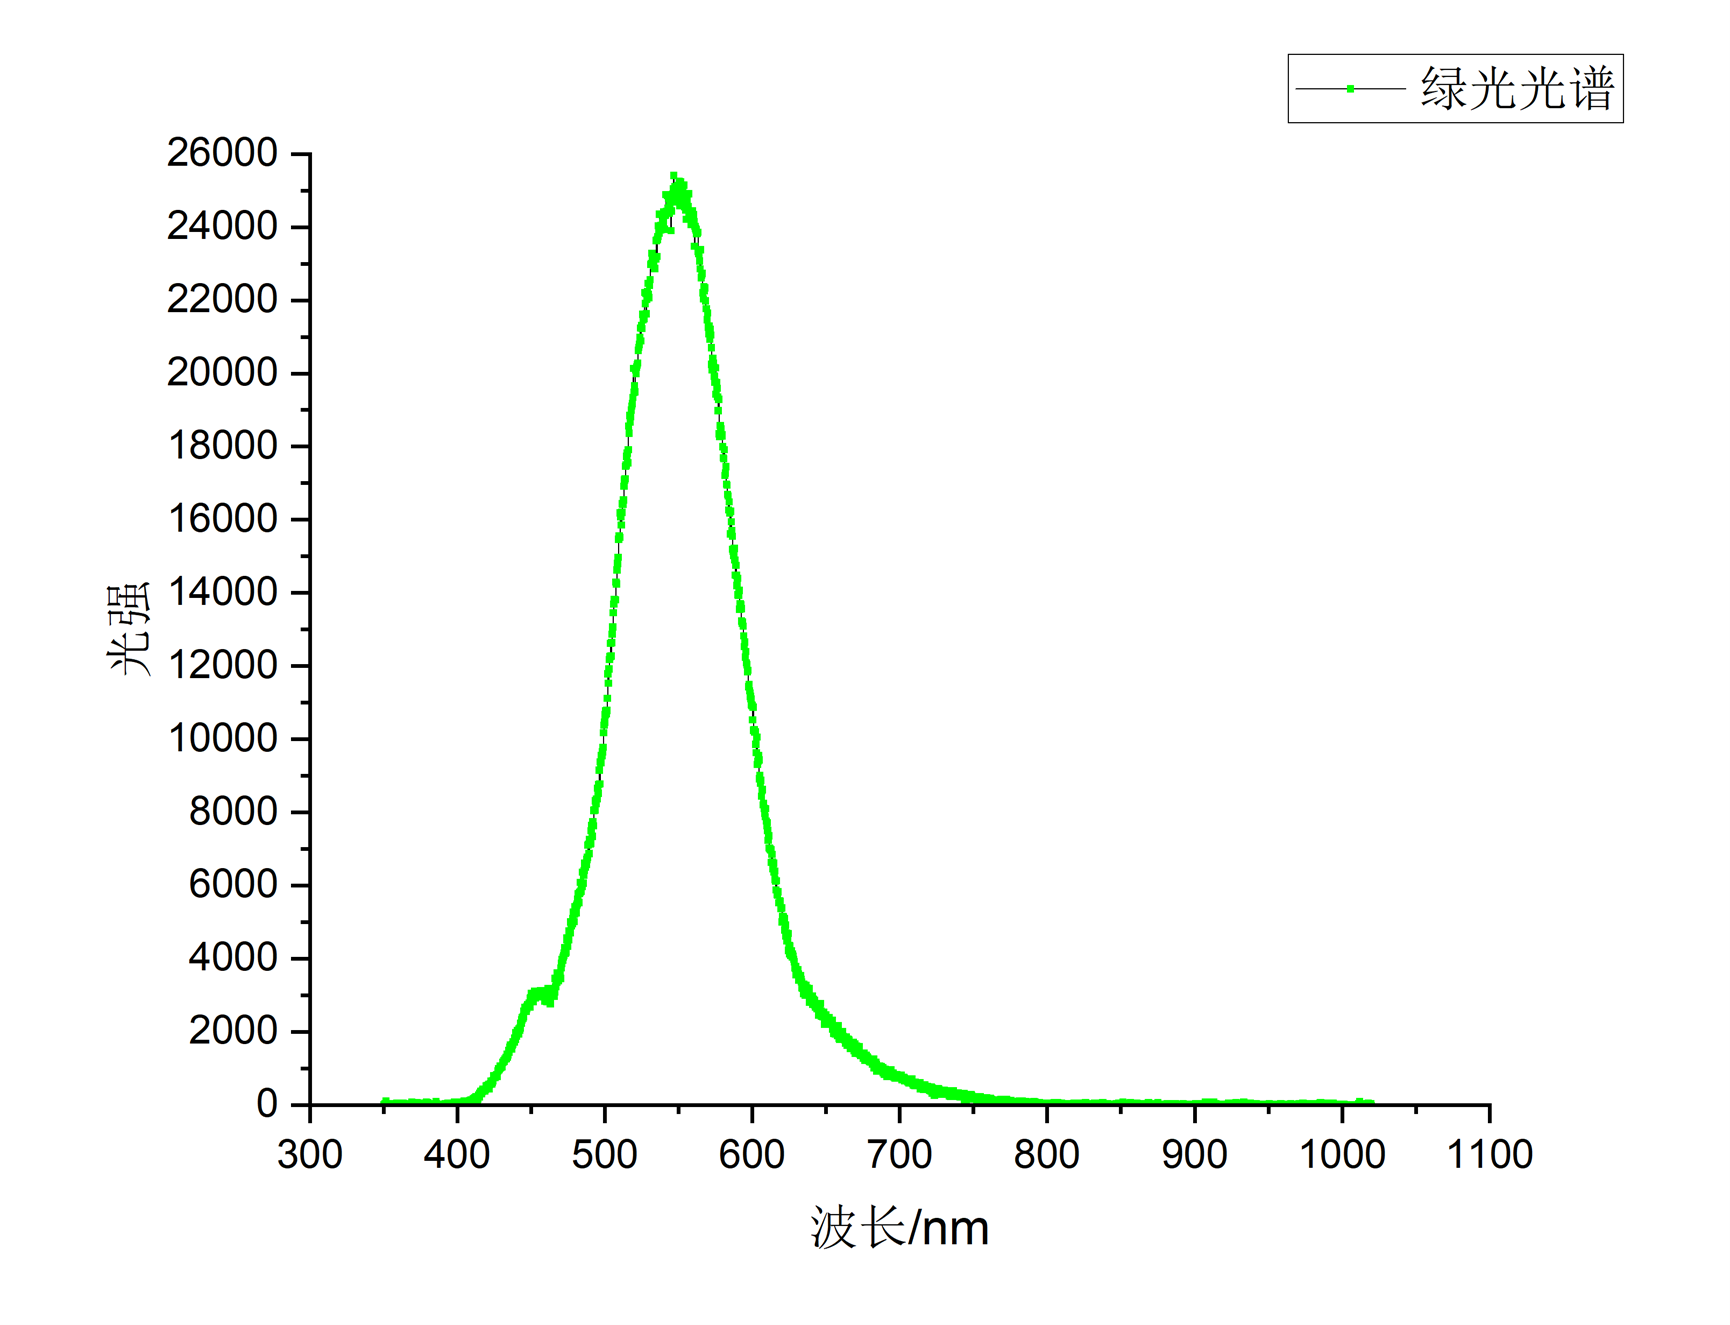
\includegraphics[width=6.5cm]{Fig/25-绿.png}
            \caption{处理绿光光谱}
        \end{minipage}
    \end{figure}
    \par \hspace*{2em}处理中,处理掉光强小于0的部分。所得图像与经验大致一致,色光的异常小波峰可能是外界光影响。
    
\end{enumerate}
\section{实验反思、收获与总结}
\begin{enumerate}
    \item 光路实验中,准直仍旧是最重要的部分。
    \item 手刻高通滤纸/假彩色滤纸时,要刻准。高通滤纸要刻孔大一点,假彩色滤纸可以多刻几个条带,降低单条带误差。
\end{enumerate}


\end{document}